%\documentclass[12pt,oneside,a4paper]{book}
\documentclass[12pt,twoside,a4paper]{book}

\usepackage[latin1]{inputenc}
\usepackage[english]{babel}
\usepackage{enumerate}
\usepackage{amsmath}
\usepackage{amssymb}
\usepackage{amsthm}
\usepackage{latexsym}
\usepackage{makeidx}
\usepackage[dvips]{graphicx}
\usepackage[bindingoffset=1cm]{geometry}
%\usepackage{showidx}
\usepackage[retainorgcmds]{IEEEtrantools}
\usepackage[toc,page]{appendix}

\makeindex

% --------------------------------------------------------------------- Symbols
\renewcommand{\phi}{\varphi}

% ------------------------------------------------------------------------ Sets
\newcommand{\N}{\mathbb{N}}
\newcommand{\R}{\mathbb{R}}
\newcommand{\Rplus}{\R^{+}}
\newcommand{\C}{\mathbb{C}}
\newcommand{\Z}{\mathbb{Z}}
\newcommand{\RS}{\hat{\C}}
\newcommand{\UnitCirc}{S^{1}}

\newcommand{\Words}[1]{{#1}^{\star}}

\newcommand{\GL}[1]{\operatorname{GL}_2(#1)}
\newcommand{\PGL}[1]{\operatorname{PGL}_2(#1)}
\newcommand{\SL}[1]{\operatorname{SL}_2(#1)}
\newcommand{\PSL}[1]{\operatorname{PSL}_2(#1)}
\newcommand{\Mat}[3]{{#1}^{#2 \times #3}}

\newcommand{\ModGrp}{\overline{\Gamma}}
\newcommand{\hModGrp}{\Gamma}

\newcommand{\setdef}[2]{\{#1 \mid #2\}}

% ---------------------------------------------------------------------- Macros
\newcommand{\todo}[2]{\bigskip\noindent\framebox[\textwidth]{\emph{TODO #1:} #2}\bigskip}
\newcommand{\ie}{i.e.\ }
\newcommand{\Wlog}{W.l.o.g.\ }
\newcommand{\txtiff}{if and only if\ }

% ------------------------------------------------------------------- Functions
\newcommand{\half}[1]{\frac{#1}{2}}
\newcommand{\reci}[1]{\frac{1}{#1}}

\newcommand{\cfr}[2]{
\begin{array}{c}\multicolumn{1}{c|}{#1}\\
\hline\multicolumn{1}{|c}{#2}\end{array}}

\newcommand{\inv}[1]{{#1}^{-1}}

\newcommand{\moebius}[5]{\frac{#1 #5 + #2}{#3 #5 + #4}}
\newcommand{\mat}[4]{\begin{pmatrix}#1 & #2 \\ #3 & #4\end{pmatrix}}
\newcommand{\rvec}[2]{\begin{pmatrix}#1 & #2\end{pmatrix}}
\newcommand{\cvec}[2]{\begin{pmatrix}#1 \\ #2\end{pmatrix}}
\newcommand{\htransp}[1]{#1^{\textrm{H}}}
\newcommand{\id}[1]{\operatorname{id}_{#1}}

\newcommand{\abs}[1]{|#1|}
\newcommand{\conj}[1]{\overline{#1}}
\renewcommand{\Re}[1]{\operatorname{Re}\left(#1\right)}
\renewcommand{\Im}[1]{\operatorname{Im}\left(#1\right)}

\newcommand{\epo}[1]{e^{#1}}
\newcommand{\ii}{i}

% ---------------------------------------------------------------- Environments

\newtheorem{theorem}{Theorem}[chapter]
\newtheorem{corollary}[theorem]{Corollary}
\newtheorem{lemma}[theorem]{Lemma}

\theoremstyle{definition}
\newtheorem{definition}[theorem]{Definition}
\newtheorem{example}[theorem]{Example}

\theoremstyle{remark}
\newtheorem*{remark}{Remark}


\title{Computer Algebra and Analysis:\\Complex Variables Visualized}
\author{Thomas Ponweiser}
\date{\today}

\pagestyle{headings}

\begin{document}

\frontmatter

%\maketitle
\begin{titlepage}
\begin{center}

\includegraphics[width=0.5\textwidth]{tu-logo-bw}

\vspace{\stretch{1}}

{\LARGE \textsc{Diplomarbeit}}

\vspace{\stretch{1}}

{\large Computer Algebra and Analysis:}

\bigskip

{\huge \textbf{Complex Variables Visualized}}

\vspace{\stretch{1}}

{Ausgef�hrt am}

\bigskip

{\large Research Institute for Symbolic Computation (RISC)\\}

\bigskip

{der Johannes Kepler Universit�t Linz}

\vspace{\stretch{1}}

{unter Anleitung von}

\bigskip

{\large Univ.-Prof.\ Dr.\ Peter Paule}

\vspace{\stretch{1}}

{durch}

\bigskip

{\large Thomas Ponweiser}

\bigskip

{\small Stockfeld 15\\
4283 Bad Zell}

\vspace{\stretch{2}}

\end{center}

\noindent
\begin{tabular}{@{} c @{} c @{} c @{}}
\rule{0.4\textwidth}{.5pt} & \rule{0.2\textwidth}{0pt} & \rule{0.4\textwidth}{.5pt} \\
{\small Datum} & & {\small Unterschrift}
\end{tabular}

\pagebreak

\end{titlepage}


% ----------------------------------------------------------- CHAPTER: ABSTRACT
\chapter*{Kurzfassung}

Ziel dieser Diplomarbeit ist die Visualisierung einiger grundlegender Ergebnisse aus dem Umfeld der Theorie der modularen Gruppe sowie der modularen Funktionen unter Zuhilfenahme der Computer Algebra Software \emph{Mathematica}.

Die Arbeit gliedert sich in drei Teile. Im ersten Kapitel werden f�r diese Arbeit relevante Begriffe aus der Gruppentheorie wiederholt. Weiters werden M�bius Transformationen eingef�hrt und deren grundlegende geometrische Eigenschaften untersucht.

Das zweite Kapitel ist der Untersuchung der modularen Gruppe aus algebraischer und geometrischer Sicht gewidmet. Der kanonische Fundamentalbereich der modularen Gruppe sowie die daraus abgeleitete Kachelung der oberen Halbebene wird eingef�hrt. Weiters wird eine generelle Methode zum Auffinden von Fundamentalbereichen f�r Untergruppen der modularen Gruppe vorgestellt, welche sich zentral auf die Konzepte der 2-dimensionalen hyperbolischen Geometrie st�tzt.

Im dritten Kapitel geben wir einige konkrete Beispiele, wie die aufgebaute Theorie f�r die Visualisierung bestimmter mathematischer Sachverhalte angewendet werden kann. Neben der Visualisierung von Graphen modularer Funktionen stellt sich auch der Zusammenhang zwischen modularen Transformationen und Kettenbr�chen als besonders sch�nes Ergebnis dar.

\chapter*{Abstract}

The aim of this diploma thesis is the visualization of some fundamental results in the context of the theory of the modular group and modular functions. For this purpose the computer algebra software \emph{Mathematica} is utilized.

The thesis is structured in three parts. In Chapter 1, we recapitulate some important basic concepts of group theory which are relevant to this work. Moreover, we introduce M�bius transformations and study their geometric mapping properties.

Chapter 2 is devoted to the study of the modular group from an algebraic and geometric point of view. We introduce the canonical fundamental region which gives rise to the modular tessellation of the upper half-plane. Additionally, we present a general method for finding fundamental regions with respect to subgroups of the modular group based on the concepts of 2-dimensional hyperbolic geometry.

In Chapter 3 we give some concrete examples how the above results and methods can be exploited for the visualization of certain mathematical results. Besides the visualization of function graphs of modular functions, a particularly nice result is the connection between modular transformations and continued fraction expansions.



% ------------------------------------------------------- CHAPTER: INTRODUCTION
\chapter*{Preface}

The centerpiece of the present diploma thesis, \emph{Computer Algebra and Analysis: Complex Variables Visualized}, is the modular group. It plays an important role in many areas of mathematics, as for example in number theory due to its connection with partition numbers or continued fractions.

This thesis is structured in three parts. In Chapter 1, we introduce basic notions and definitions which are fundamental for the rest of this work. Firstly, we summarize the most important basic concepts of group theory. Moreover, we introduce \emph{M�bius transformations} and study their connection to \emph{stereographic projection} in detail. Finally, we define the concept of \emph{generalized circles} and \emph{generalized disks}, using an elegant characterization in terms of Hermitian matrices which turns out to be particularly advantageous in the context of M�bius transformations. 

Chapter 2 is devoted to the study of the modular group from an algebraic and geometric point of view. Two different and independent algorithms, the $T$-$U$ algorithm and the $T$-$R$ algorithm, are presented which both yield group word representations for arbitrary modular transformations in terms of the transformations $T : z \mapsto \reci{z}$, $U : z \mapsto z+1$ and $R : z \mapsto \reci{z+1}$. Geometric considerations come into play when introducing \emph{fundamental regions} for the action of the modular group on the extended complex plane. A canonical fundamental region is derived which gives rise to the \emph{modular tessellation of the upper-half plane}. Lastly, the basic concepts of 2-dimensional \emph{hyperbolic geometry} are introduced in order to present an alternative and more general method for finding fundamental regions. This method gives rise to so-called \emph{normal polygons} and works as well for subgroups of the modular group.

Finally, Chapter 3 has a clear emphasis on visualization. Firstly, \emph{generalized matrix powers} are introduced as a device for visualizing continuous transitions between given sets and their M�bius-transformed images. Secondly, the relation between the modular transformations, \emph{Ford circles} and \emph{continued fractions} is studied in detail and visually explained using the continued fraction expansion of the irrational number $\pi$ as an example. Lastly, documenting the important role of the modular group within complex analysis, the most basic results from the theory of \emph{modular functions} are summarized. Using an adequate color coding, graphs of certain selected modular functions are depicted whose inherent visual aesthetics and symmetry reflect well the beauty of this theory.

\section*{Achievements}

Complementary to this thesis, the \emph{Mathematica} package \emph{ModularGroup} has been developed. This package, together with some \emph{interactive demonstrations}, may be downloaded from the website of the \emph{Research Institute for Symbolic Computation} (RISC).\footnote{http://www.risc.jku.at/} It contains essentially all algorithms described in this thesis as well as functions for visualization of generalized circles, generalized disks, modular tessellations and more. The main attention has been paid to an efficient and fast implementation of these algorithms, relying in many aspects on compiled functions using machine-precision integer and floating point arithmetic. Note that all figures included in this thesis are based on this package. 

Furthermore it is worth noting that this thesis also contains ideas which have not been found directly in this form in the referenced literature. During the implementation of the enumeration algorithm for modular transformations, it got apparent that the left- or rightmost symbol of the unique $T$-$R$ group word of any given modular transformation can be read off directly from its corresponding matrix. This observation leads to the $T$-$R$ algorithm of Section~\ref{sec_ModularGroupGenRel} and to the alternative proof for the presentation for the modular group in terms of the generators $T$ and $R$ (Theorem~\ref{thm_ModGrpTRProd}). 

For the proof that the region $\FunDom := \setdef{z \in \C}{\abs{\Re{z}} < 1 \land \abs{z} > 1}$ is a fundamental region for the action of the modular group on the upper half-plane, we intentionally take a different and slightly longer track than for example \Klein{} or \Schoeneberg{}. We first derive a fundamental region for the action of the homogeneous modular group on $\C^2$ by looking for representative vectors of minimal Euclidean norm. By carrying over the result to the inhomogeneous case, we indeed obtain the fundamental region $\FunDom$ in a very natural and instructive way.

%As the Euclidean algorithm prominently appears at several different places within this thesis, we take into account that there is more than one ``Euclidean algorithm'', depending on the chosen method for integer divison.

For visualization of objects living on the upper half-plane of $\C$, such as the modular tessellation or graphs of modular functions, we frequently make use of a M�bius transformation which maps the upper half-plane to the unit disk. This allows us to visualize the whole picture rather than just an arbitrary rectangular fragment of it. It turns out that in this context the most natural choice for such a M�bius transformation is \emph{not} the well-known Cayley transform, but in fact a map which we introduce in Example~\ref{ex_ModCayleyTransform} as the \emph{modified Cayley transform}.

%For visualization of continuous transitions between sets and their M�bius-transformed images, \emph{generalized matrix powers} which are available as undocumented feature in \emph{Mathematica}'s built-in function \emph{MatrixPower} have been formalized in Section~\ref{sec_ActionVisu}.

Another idea suggesting itself is to consider the inscribed circle of the canonical fundamental region $\FunDom$ (see Figure~\ref{fig_PSL2FunDom}). Indeed, the introduction of so-called \emph{indisks} turns out to be very fruitful in the study of the relation between modular transformations and continued fractions in Section~\ref{sec_ConFrac}. It leads to the notion of \emph{indisk-paths}, which in turn give rise to an alternative proof for the presentation of the modular group in terms of the generators $T$ and $R$ (Corollary~\ref{cor_TRRelationsIndiskPaths}).

\section*{Outlook}

The \emph{Mathematica} package \emph{ModularGroup} may be extended for a systematic treatment of various congruence subgroups of the modular group. The algorithm which has been used for drawing the \emph{normal polygons} in Section~\ref{sec_NormalPolygons} has been one of the latest results of this work. It is still preliminary and may be added to the package at a later stage.

Also the implementation of H.\ A.\ Verrill's algorithm for the visualization of fundamental regions of congruence subgroups\footnote{See https://www.math.lsu.edu/$\sim$verrill/} -- which has actually been the starting point for this thesis -- is easily possible based on the present \emph{Mathematica} package.

\section*{Acknowledgment}

I want to thank everybody who supported me in the course of my work on this  diploma thesis. 

I am particularly grateful to my supervisor \emph{Prof.\ Peter Paule} for proposing this truly rewarding topic and its neat working title. I very much appreciated his valuable input and guidance as well as our constructive project meetings.

My special thanks also go to \emph{Prof.\ G�nther Karigl} for his prompt and kind answers to my administrative questions and for approving this thesis at the Research Institute for Symbolic Computation of the Johannes Kepler University Linz.

Last but not least I want to thank my family for supporting me. Thanks to my little daughter Lisa for being my sunshine and reminding me of the importance of baby steps. To my beloved wife I want to say thank you for always motivating me. Thank you for being the wind in my sails!


\tableofcontents

\listoffigures

\mainmatter
% ------------------------------------------------------------- CHAPTER: BASICS
\chapter{Basic notions and definitions}

% -------------------------------------------- Section: Algebraic constructions
\section{Groups and basic algebraic constructions}

In this section, we will recapitulate some basic algebraic concepts, most important the notions of \emph{free groups} and \emph{free products}, and the construction of a group in terms of \emph{generators} and \emph{relations}. Additionally, we give the definitions of the \emph{(projective) general} and \emph{special linear groups}. Lastly, \emph{group actions} on sets will be introduced. A reader familiar to this concepts may readily skip this section. Moreover, we will give no rigorous proofs here, as they may be found in many algebra books, as for example in \Hungerford.

\subsection{Groups and homomorphisms}

\index{Binary!operation}
If $G$ is a nonempty set, a \emph{binary operation} on $G$ is a function $G \times G \to G$. Commonly used notations for the image of $(a,b) \in G \times G$ under a binary operation are $a \cdot b$ or $ab$ (product notation), $a + b$ (additive notation), $a \circ b$, $a \ast b$, etc. In this chapter and also later on we will use the \emph{product notation}, $(a,b) \mapsto a \cdot b =  ab$, most frequently and we refer to $ab$ as the \emph{product} of $a$ and $b$.

\begin{definition}[Groups and monoids]
\label{dfn_GroupMonoid}
\index{Group}
\index{Monoid}
Let $G$ be a nonempty set together with a binary operation on $G$. If the binary operation satisfies the following three axioms,
\index{Associativity}
\begin{enumerate}[(i)]
\item \label{itm_Associativity} \emph{Associativity:} $\forall a,b,c \in G: a(bc) = (ab)c$,
\item \label{itm_IdentityExists} \emph{Existence of an identity element:} $\exists e \in G\ \forall a \in G: ea = ae = a$,
\item \emph{Existence of inverse elements:} $\forall a \in G\ \exists \inv{a} \in G: a \inv{a} = \inv{a} a = e$,
\end{enumerate}
then $G$ is called a \emph{group}. If the axioms (\ref{itm_Associativity}) and (\ref{itm_IdentityExists}) are satisfied, then $G$ is called a \emph{monoid}. Of course every group is in particular monoid. The notation $\langle G,\cdot,e \rangle$ will be used for making the identity element and the involved binary operation explicit.
\end{definition}

It is convenient to introduce the following notations operating on subsets of a group $G$. For $g \in G$ and $A,B \subseteq G$ we define
\begin{eqnarray*}
\inv{A} &:=& \setdef{\inv{a}}{a \in A} \subseteq G, \\
AB &:=& \setdef{a b}{a \in A, b \in B} \subseteq G,\\
gA &:=& \{g\}A = \setdef{g a}{a \in A} \subseteq G,\\
Ag &:=& A\{g\} = \setdef{a g}{a \in A} \subseteq G.
\end{eqnarray*}

\begin{definition}[Subgroups]
\label{dfn_Subgroup}
\index{Subgroup}
Let $\langle G,\cdot,e \rangle$ be a group. A nonempty subset $H \subseteq G$ which is closed under the binary operation $\cdot$ and inversion, \ie $H\inv{H} = H$, is called a \emph{subgroup} of $G$, in symbols $H \le G$. In particular, $\langle H,\cdot,e \rangle$ is itself a group. If $H \le G$ and $H \ne G$, $H$ is called a \emph{proper subgroup} of $G$, and we write $H \lneq G$. The subgroup $\{e\} \le G$ is called the \emph{trivial subgroup}.
\end{definition}

\index{Conjuagtion}
If $H$ is a subgroup of $G$, then for every $g \in G$ also $gH\inv{g}$ is a subgroup of $G$. For $h \in H$, $g \in G$, we call the operation $h \mapsto g h \inv{g}$ \emph{conjugation} of $h$ by $g$.

\begin{definition}[Normal subgroups]
\label{dfn_NormalSubgroup}
A subgroup $N$ of a group $G$ which is closed under conjugation by elements of $G$, \ie $g N \inv{g} = N$ for all $g \in G$, is called a \emph{normal subgroup} of $G$, in symbols $N \unlhd G$.
\end{definition}

If $N$ is a normal subgroup of $G$, then we have $gN = Ng$ for every $g \in G$, which is why we can define on the set
\begin{equation}
\label{eqn_FactorGroup}
G / N := \setdef{gN}{g \in G}
\end{equation}
a binary operation by $aNbN := abNN = abN$ for $a,b \in G$. It is easy to see that $G / N$ together with this operation forms a group.

\begin{definition}[Factor groups]
\label{dfn_FactorGroup}
Let $N$ be a normal subgroup of a group $G$. The set $G / N$ defined in (\ref{eqn_FactorGroup}) together with the binary operation $(aN,bN) \mapsto abN$ is called the \emph{factor group} (or \emph{quotient group}) of $G$ by $N$.
\end{definition}

\begin{definition}[Homomorphisms]
\label{dfn_Homomorphism}
\index{Homomorphism}
\index{Monomorphism}
\index{Epimorphism}
\index{Isomorphism}
\index{Endomorphism}
\index{Automorphism}
Let $G$ and $H$ be groups (or monoids). A function $f : G \to H$ is a \emph{homomorphism} from $G$ to $H$, if and only if
\begin{equation*}
f(ab) = f(a) f(b) \quad \text{for all } a,b \in G.
\end{equation*}
Depending on $f$ being injective and/or surjective, one distinguishes \emph{monomorphisms} ($f$ is injective), \emph{epimorphisms} ($f$ is surjective) and \emph{isomorphisms} ($f$ is bijective). We call the groups $G$ and $H$ \emph{isomorphic}, in symbols $G \cong H$, if and only if there exists and isomorphism $f : G \to H$. Finally, a homomorphism $f : G \to G$ of $G$ to itself is called \emph{endomorphism}. A bijective endomorphism is called \emph{automorphism}.
\end{definition}

\begin{definition}[Kernel]
\label{dfn_Kernel}
Let $G$ and $H$ be groups and denote the identity element of $H$ by $e_H$. For a homomorphism $f: G \to H$, the set
\begin{equation}
\ker f := \setdef{g \in G}{f(g) = e_H}
\end{equation}
is called the \emph{kernel} of f.
\end{definition}
\begin{lemma}
\label{lem_KernelAndImage}
Let $G$ and $H$ be groups and $f : G \to H$ be a homomorphism. The kernel of $f$ is a normal subgroup of $G$ and the image $f(G)$ is a subgroup of $H$:
\begin{equation*}
\ker f \unlhd G \quad \text{and} \quad f(G) \le H.
\end{equation*}
\end{lemma}
\begin{proof}
Denote the identity elements of $G$ and $H$ by $e_G$ and $e_H$ respectively. Because $f$ is a homomorphism, we have $f(e_G) = f(e_G e_G) = f(e_G) f(e_G)$. Multiplying this by $\inv{f(e_G)}$ yields $e_H = f(e_G)$. In other words $e_G \in \ker f$ and $\ker f$ is nonempty. To see that $\ker f \le G$, we need to show that for all $a, b \in \ker f$ also $a \inv{b} \in \ker f$ -- but this is easy:
\begin{equation*}
f(a \inv{b}) = f(a) f(\inv{b}) = f(a) \inv{f(b)} = e_H \inv{e_H} = e_H.
\end{equation*}
To see that $\ker f$ is a normal subgroup of $G$, let $a \in \ker f$, $g \in G$ and observe
\begin{equation*}
f(g a \inv{g}) = f(g) f(a) f(\inv{g}) = f(g) e_H \inv{f(g)} = e_H.
\end{equation*}
For this reason $g a \inv{g} \in \ker f$ and $\ker f$ is closed under conjugation by elements of $G$. For the second part of the prove, let $f(a), f(b) \in f(G)$ with $a,b \in G$. Clearly $f(a) \inv{f(b)} = f(a) f(\inv{b}) = f(a \inv{b}) \in f(G)$ and therefore $f(G) \le H$.
\end{proof}

\begin{theorem}[First isomorphism theorem]
\label{thm_FirstIsoThm}
Let $G$ and $H$ be groups and $f: G \to H$ be a homomorphism. Then the quotient group $G / \ker f$ is isomorphic to $f(G)$:
\begin{equation*}
G / \ker f \cong f(G).
\end{equation*}
\end{theorem}
\begin{proof}
Let us again denote the identity element of $H$ by $e_H$. Define $N := \ker f$ and a map $\phi : G/N \to f(G)$ by $aN \mapsto f(a)$. Now, for arbitrary $a,b \in G$ observe
\begin{equation*}
aN = bN \Leftrightarrow
a \inv{b} \in N \Leftrightarrow
e_H = f(a \inv{b}) = f(a) \inv{f(b)} \Leftrightarrow
f(a) = f(b).
\end{equation*}
This shows two things: First ($\Rightarrow$), $\phi$ is well defined and second ($\Leftarrow$), $\phi$ is injective. Clearly, $\phi$ is also surjective and by definition we have
\begin{equation*}
\phi(aN) \phi(bN) = f(a) f(b) = f(ab) = \phi(abN) \quad \text{for all } a,b \in G.
\end{equation*}
Therefore $\phi$ is indeed an isomorphism from $G/N$ to $f(G)$.
\end{proof}

\subsection{Free monoids}
\index{Free!monoid}
Let $\Syms$ be a set of formal symbols, for example $\Syms = \{a, b, c, \dots\}$. For $n \in \N$, $n \ge 0$, we denote by $\Syms^n$ the set of tuples of length $n$ over $\Syms$ and we will call these tuples \emph{words of length $n$ over the alphabet $\Syms$}. For simplicity, we will omit parentheses and commas when notating such a word, for example $(a,b,b,a) =: abba \in \Syms^4$ is a word of length 4. Note the special case for $n = 0$. By definition, $\Syms^0$ contains all words of length $0$. Obviously, there is only one such word, the so-called \emph{empty word}, which we denote by $\epsilon$. A second special case occurs for $\Syms = \emptyset$, where $\Syms^n = \emptyset$ for all $n > 0$ and $\Syms^0 = \{\epsilon\}$, because there are no words over the empty alphabet except the empty word. Next, we define 
\begin{equation}
\label{eqn_SigmaStarDef}
\Words{\Syms} := \bigcup_{n \ge 0} \Syms^n.
\end{equation}
as the set of all \emph{words over the alphabet $\Syms$}. It is now just natural to define a binary operation $\cdot$ on $\Words{\Syms}$ which is given by concatenation of words:
\begin{equation*}
w_1 \cdot w_2 := w_1 w_2, \quad w_1, w_2 \in \Words{\Syms}.
\end{equation*}
\index{Monoid}
Since $\Words{\Syms}$ together with the operation $\cdot$ satisfies the axioms of \emph{associativity},
\begin{equation*}
\forall w_1,w_2,w_3 \in \Words{\Syms}:\quad (w_1 \cdot w_2) \cdot w_3 = w_1 \cdot (w_2 \cdot w_3)
\end{equation*}
and \emph{existence of an identity element},
\begin{equation*}
\forall w \in \Words{\Syms}:\quad w \cdot  \epsilon = \epsilon \cdot w = w,
\end{equation*}
the algebraic structure $\langle \Words{\Syms}, \cdot, \epsilon \rangle$ forms a \emph{monoid}.

\begin{definition}[Free monoid]
\label{dfn_FreeMonoid}
Let $\Syms$ be an arbitrary set of symbols (called the alphabet), and $\Words{\Syms}$ be defined as in (\ref{eqn_SigmaStarDef}). Moreover, denote concatenation of words by $\cdot$ and let $\epsilon$ be the empty word. Then the algebraic structure $\langle \Words{\Syms}, \cdot, \epsilon \rangle$ is called the \emph{free monoid over the alphabet $\Syms$}.
\end{definition} 

\subsection{Free groups}
\index{Free!group}
\index{Formal!inverse}
In a similar fashion, we can construct also a group from any given formal alphabet $\Syms$. For this purpose we first choose a ``disjoint copy'' of $\Syms$ which we denote by $\inv{\Syms}$. To be precise, $\inv{\Syms}$ may be any arbitrary set satisfying $\Syms \cap \inv{\Syms} = \emptyset$ and having same cardinality as $\Syms$. In particular we could for example set $\inv{\Syms} := \Syms \times \{1\}$. Next, we choose a bijection $f : \Syms \to \inv{\Syms}$. We can extend this bijection between the sets $\Syms$ and $\inv{\Syms}$ to an involution $\overline{f}$ living on the union $\overline{\Syms} := \Syms \cup \inv{\Syms}$ by defining $\overline{f} := f \cup \inv{f}$ or more verbose:
\begin{equation*}
\overline{f}(a) := \begin{cases}
f(a)       & \text{if } a \in \Syms\\
\inv{f}(a) & \text{if } a \in \inv{\Syms}
\end{cases}
\end{equation*}
Now we introduce the notation $\overline{f}(a) =: \inv{a}$ for all $a \in \overline{\Syms}$ and call $\inv{a}$ the \emph{(formal) inverse} of the element $a$. 

\index{Reduced form}
\index{Group!word}
Having now defined a formal inverse for each of our symbols in the given alphabet, we can go on and consider the free monoid $\Words{\overline{\Syms}}$. If $\sigma_1, \sigma_2, \dots, \sigma_n$ are symbols of $\overline{\Syms}$, then we say the word $\sigma_1 \sigma_2 \dots \sigma_n$ is \emph{reduced}, if and only if no two subsequent symbols of the word are inverse to each other, that is
\begin{equation}
\label{eqn_GrpWordReducedForm}
 \sigma_j \ne \sigma_{j+1}^{-1} \quad \text{for all } 1 \le j < n.
\end{equation}
Clearly, every word $w \in \Words{\overline{\Syms}}$ can be brought into reduced form by successively ``canceling out'' adjacent inverse symbols until finally a word is obtained, which satisfies (\ref{eqn_GrpWordReducedForm}). We call the result of this procedure the \emph{reduced form of $w$}. Additionally, we define two words $w_1, w_2 \in \Words{\overline{\Syms}}$ to be \emph{equivalent}, if and only if they have the same reduced form and we write $w_1 \sim w_2$ in this case. If we denote the reduced form of $w$ by $\phi(w)$, we can write
\begin{equation*}
w_1 \sim w_2 \Leftrightarrow \phi(w_1) = \phi(w_2).
\end{equation*}
Moreover, we observe that if $w_1 \sim w_2$ and $v_1 \sim v_2$, then we also have $w_1 v_1 \sim w_2 v_2$ because $\phi(w_1) = \phi(w_2) =: w$ and $\phi(v_1) = \phi(v_2) =: v$ implies 
\begin{equation*}
\phi(w_1 v_1) = \phi(w v) = \phi(w_2 v_2).
\end{equation*}
Thus we see that the equivalence relation $\sim$ is compatible with the operation of word-concatenation. Therefore we can consider also the set of equivalence classes $\Words{\overline{\Syms}}/{\sim}$ as a monoid under the operation of word-concatenation. Obviously the set of reduced words is a system of representatives for $\Words{\overline{\Syms}}/{\sim}$ and we agree to denote an equivalence class $[w]_{\sim}$ simply by the reduced word $w$. $\Words{\overline{\Syms}}/{\sim}$ is not just a monoid, but in fact a group, as the inverse of a word $\sigma_1 \sigma_2 \dots \sigma_{n-1} \sigma_n$ is trivially given by $\sigma_n^{-1} \sigma_{n-1}^{-1} \dots \sigma_2^{-1} \sigma_1^{-1}$. We call a reduced word of $\Words{\overline{\Syms}}$ (resp. its corresponding equivalence class in $\Words{\overline{\Syms}}/{\sim}$) a \emph{group word over the alphabet $\Syms$}.

\begin{definition}[Free group]
\label{dfn_FreeGroup}
Let $\Syms$ be an arbitrary set of formal symbols and define $\overline{\Syms} := \Syms \cup \inv{\Syms}$ as above. On the free monoid $\Words{\overline{\Syms}}$ define an equivalence relation $\sim$ by identifying words with the same reduced form. Then the algebraic structure 
\begin{equation}
\label{eqn_FreeGrp}
\FreeGrp{\Syms} := \langle \Words{\overline{\Syms}}/{\sim}, \cdot, \epsilon \rangle
\end{equation}
is called the \emph{free group over the alphabet $\Syms$}.
\end{definition}

\begin{remark}
In the exceptional case, when $\Syms = \emptyset$,  we obtain the trivial group by this construction: Namely, if $\Syms = \emptyset$ then we can also choose $\inv{\Syms} = \emptyset$ ($\Syms$ and $\inv{\Syms}$ are then disjoint as required). It follows that also $\overline{\Syms}$ is empty and we end up with the trivial monoid $\Words{\overline{\Syms}} = \{\epsilon\}$, which corresponds to the trivial group.
\end{remark}

\begin{example}
Let $\Syms$ be the singleton set $\{a\}$. Now, the free group over $\Syms$ consists precisely of the following group words:
\begin{equation*}
\FreeGrp{\Syms} = \{\epsilon, a, aa, aaa, \dots, \inv{a}, \inv{a}\inv{a},\dots\}.
\end{equation*}
If we now introduce the notation
\begin{equation*}
\epsilon =: a^0, \quad 
\underbrace{a a \dots a}_{k \text{ times}} =: a^k, \quad
\underbrace{\inv{a} \inv{a} \dots \inv{a}}_{k \text{ times}} =: a^{-k},
\end{equation*}
we have $a^n \cdot a^m = a^{n+m}$ for all $n,m \in \Z$ and it is thus evident that the free group over any one-element alphabet is isomorphic to the group $\langle \Z, +, 0 \rangle$. 

Note that this is the only case (besides the trivial one, when $\Syms = \emptyset$), where the free group is commutative. In fact, the free group construction always yields a group with ``richest possible'' structure in the following sense:

\begin{theorem}
\label{thm_FreeGrpUniqueHom}
Let $\Syms$ be an arbitrary set and $G$ be an arbitrary group. If any mapping $\phi : \Syms \to G$ is given, then we can always extend $\phi$ in a unique way to a homomorphism $\overline{\phi}: \FreeGrp{\Syms} \to G$.
\end{theorem}

In fact, the property described in Theorem \ref{thm_FreeGrpUniqueHom} completely characterizes the free group up to isomorphism, as stated in the next Theorem:

\begin{theorem}[Universal mapping property]
\label{thm_FreeGrpUnivMapProp}
Let $\Syms$ be an arbitrary set and $F$ be a group together with an injective map $\iota : \Syms \to F$. If $F$ has the property that for any map $\phi : \Syms \to G$, where $G$ is an arbitrary group, there is a homomorphism $\overline{\phi} : F \to G$ such that $\phi = \overline{\phi} \circ \iota$,
then $F$ is (isomorphic to) the free group over the alphabet $\Syms$.
\end{theorem}

\end{example}

\subsection{Generators and relations}

\begin{definition}
\index{Generator}
\index{Group!generator}
Let $\langle G, \cdot, 1 \rangle$ be a group and $\Syms \subseteq G$ a subset. We say $G$ is \emph{generated by} the elements of $\Syms$, if every element $g \in G$ can be written as a product of elements from $\Syms$ in the following sense:
\begin{equation}
\label{eqn_GrpGenerators}
\forall g \in G\ \exists n \in \N,\ (\sigma_j) \in \Syms^n,\ (k_j) \in \Z^n:\quad 
g = \sigma_1^{k_1} \sigma_2^{k_2} \dots \sigma_n^{k_n}.
\end{equation}
Moreover, in this case we call the elements of $\Syms$ \emph{generators} of $G$. 
\end{definition}

\index{Group!relation}
Let us first consider the case, when some $g \in G$ can be generated in two  different ways, for example
\begin{equation*}
g = \sigma_1^{k_1} \sigma_2^{k_2} \dots \sigma_n^{k_n} 
  = \tau_1^{\ell_1} \tau_2^{\ell_2} \dots \tau_m^{\ell_m}
\end{equation*}
with $\sigma_j, \tau_j \in \Syms$ and $k_j, \ell_j \in \Z$. This immediately gives
\begin{equation}
\label{eqn_GrpRelation}
\sigma_1^{k_1} \sigma_2^{k_e} \dots \sigma_n^{k_n} \cdot
\tau_m^{-\ell_m} \tau_{m-1}^{-\ell_{m-1}} \dots \tau_1^{-\ell_1} = 1.
\end{equation}
We call the group word occurring on the left hand side of (\ref{eqn_GrpRelation}) a \emph{relation} on $G$. The set of all such possible relations on $G$ forms a normal subgroup of $\FreeGrp{\Syms}$. To see this, let $\phi : \Syms \to G$ be the canonical embedding. According to Theorem~\ref{thm_FreeGrpUniqueHom} there exists a unique extension of $\phi$ to a homomorphism $\overline{\phi}: \FreeGrp{\Syms} \to G$. In fact, this homomorphism just evaluates group words over $\Syms$ in the obvious way to concrete group elements in $G$. By definition, the set of all relations on $G$ is now given by $N := \ker(\overline{\phi})$ which is, by Lemma~\ref{lem_KernelAndImage}, a normal subgroup of $\FreeGrp{\Syms}$. It now follows from the first isomorphism theorem (Theorem~\ref{thm_FirstIsoThm}) that $G \cong \FreeGrp{\Syms} / N$. In the case, when the product representation in (\ref{eqn_GrpGenerators}) is unique for all $g \in G$, then $N$ just consists of the identity element and $G$ is isomorphic to $\FreeGrp{\Syms}$. In this case, $G$ is said to be \emph{relation-free}, which is where the terminology ``free group'' actually comes from. 

Summing up, we see that every group can be described by supplying a set of generators $\Syms$ and a the set of relations $N \unlhd \FreeGrp{\Syms}$. Of course, it is also sufficient to supply just a subset $R$ of relations from which the other relations can be derived. This leads to the following definition:

\begin{definition}[Presentation of a group]
\label{dfn_GrpConstructGenRel}
Let $\Syms$ be an arbitrary set and $R \subseteq \FreeGrp{\Syms}$ a set of group words over the alphabet $\Syms$. A group $G$ is said to be the \emph{group defined by} the \emph{generators} $\sigma \in \Syms$ \emph{and relations} $R$, if $G$ is obtained by the following construction:
\begin{enumerate}
\item Let $N$ be the normal subgroup of $\FreeGrp{\Syms}$ generated by the relations $R$:
\begin{equation*}
N := \bigcap_{R \subseteq N^{\prime} \unlhd \FreeGrp{\Syms}} N^{\prime}.
\end{equation*}
\item Define $G := \presentation{\Syms}{R} := \FreeGrp{\Syms}/N$.
\end{enumerate}
Finally, $\presentation{\Syms}{R}$ is called a \emph{presentation} of $G$.
\end{definition}

For easier notation, we may omit braces when listing $\Syms$ and $R$ in a presentation of $G$. Moreover, we may write out relations more explicitly, for example instead of $G = \presentation{\{a\}}{\{a^2\}}$ we may write $G = \presentation{a}{a^2 = 1}$.

\begin{remark}
\index{Word problem}
The presentation $\presentation{\Syms}{R}$ of a group $G$ is by far not unique as the normal group $N$ can be generated by many different subsets $R \subseteq N$. Even worse, the $\emph{word problem}$, \ie the question, if a given group word $w \in \FreeGrp{\Syms}$ is in $N$ when $R$ is given, is in general not decidable, which means that there is no general algorithm for deciding, if two given group words represent the same element of $G$.
\end{remark}

\begin{example}
The group $\presentation{t,r}{t^2 = r^3 = 1}$ consists of all group words of the form
\begin{equation*}
\label{ex_RTGroup}
r^{k_1} t r^{k_2} t \dots t r^{k_n}, \quad 
\text {with } k_1, k_n \in \{0,\pm 1\} \text{ and } k_2, \dots, k_{n-1} \in \{\pm 1\}.
\end{equation*}
\end{example}
We conclude this section with the statement, that among all groups, which satisfy a given set of relations $R$, the group constructed as above is in a certain sense the largest possible one.

\begin{theorem}
Let $\presentation{\Syms}{R}$ be a presentation of the group $G$. If $H$ is any group generated by $\Syms$ and if $H$ satisfies all relations $R$, then there is an unique epimorphism $G \to H$.
\end{theorem}

\subsection{Free products}

\index{Free!product}
Let $\langle G_i, \cdot, e_i \rangle_{i \in I}$ a family of pairwise disjoint groups, \ie $G_i \cap G_j = \emptyset$ for $i \ne j$. We define the \emph{free product} of the family of groups $(G_i)_{i \in I}$ by a construction in terms of generators and relations (see Definition~\ref{dfn_GrpConstructGenRel}) as follows. As the set of generators we choose the alphabet $\Syms = \bigcup_{i \in I} G_i$ and as the set of relations we take all the relations coming from any of the groups $G_i$. Note that a priori the neutral elements $e_i \in G_i$ are all different symbols, but the final factorization by the normal subgroup $N$ automatically identifies them with each other, as $N$ includes all the $e_i$ as trivial relations.

\begin{definition}[Free product]
Let $(G_i)_{i \in I}$ be a family of disjoint groups. For every $i \in I$, let $\overline{\phi}_i$ be the unique extension of the identity map on $G_i$ to a homomorphism $\FreeGrp{G_i} \to G_i$ according to Theorem~\ref{thm_FreeGrpUniqueHom}.\footnote{In other words, $\overline{\phi}_i$ is the map which evaluates group words over the alphabet $G_i$ to concrete elements of $G_i$ in the obvious way.} The \emph{free product} of the family $(G_i)_{i \in I}$ is defined as
\begin{equation*}
{\prod_{i \in I}}^{\star} G_i := \presentation{\Syms}{R}, 
\quad \text{where } \Syms = \bigcup_{i \in I} G_i \text{ and } R = \bigcup_{i \in I} \ker \overline{\phi}_i.
\end{equation*} 
\end{definition}

If only a small finite number of groups is involved, for example only the two groups $G$ and $H$, we will write $G \ast H$ for their free product.

\begin{example}
\label{ex_RTFreeProd}
The free product of the groups $G = \presentation{t}{t^2 = 1}$ and $H = \presentation{r}{r^3 = 1}$ is the group $G \ast H = \presentation{t,r}{t^2 = r^3 = 1}$ which we have already seen in Example \ref{ex_RTGroup}.
\end{example}

\begin{example}
Let $F_n$ and $F_m$ be the free groups generated by $n$ and $m$ elements respectively. Then the free product $F_n \ast F_m = F_{n+m}$ is the free group generated by $n+m$ elements.
\end{example}

\subsection{Basic linear groups}
In this section, we give the definitions of some important basic groups, which will be needed throughout this document. We start with the general and special linear group.

\begin{definition}[General linear group]
\label{dfn_GenLinGrp}
\index{General linear group}
\index{GLnF@$\GLn{n}{F}$}
Let $F$ be a field and $n > 0$. The group of invertible $n$-by-$n$ matrices over  $F$ is called \emph{general linear group} and is denoted by
\begin{equation}
\label{eqn_GeneralLinearGroup}
\GLn{n}{F} := \setdef{M \in \SqMat{F}{n}}{\det M \ne 0}.
\end{equation}
\end{definition}

\begin{definition}[Special linear group]
\label{dfn_SpLinGrp}
\index{Special linear group}
\index{SLnR@$\SLn{n}{R}$}
Let $R$ be a commutative ring with 1 and $n > 0$. The group of $n$-by-$n$ matrices over $R$ having determinant 1, is called \emph{special linear group} and is denoted by
\begin{equation}
\label{eqn_SpecialLinearGroup}
\SLn{n}{R} := \setdef{M \in \SqMat{R}{n}}{\det M = 1}.
\end{equation}
Of course in the case, when $R$ is contained in the field $F$, then the special linear group $\SLn{n}{R}$ is a subgroup of the general linear group $\GLn{n}{F}$. 
\end{definition}

\index{Group!center}
For both, the general and special linear group, one can construct the \emph{projective groups} by identifying matrices which differ by a scalar multiple. For this purpose, we define the \emph{center} of a group $G$ in the usual way:
\begin{equation}
\Center{G} := \setdef{z \in G}{zg = gz \quad \forall g \in G}.
\end{equation}
If $G$ is a matrix group, $\Center{G}$ consists precisely of all scalar multiples of the identity matrix within $G$, which is exactly what we need for this construction.

\begin{definition}[Projective linear groups]
\label{dfn_ProjLinGrp}
\index{Projective!general linear group}
\index{PGLnF@$\PGLn{n}{F}$}
\index{Projective!special linear group}
\index{PSLnR@$\PSLn{n}{R}$}
As above, let $F$ be a field, $R$ a ring with 1 and $n > 0$. The \emph{projective general linear group} and the \emph{projective special linear group} are defined as
\begin{IEEEeqnarray}{rClCl}
\label{eqn_ProjGenLinGrp}
\PGLn{n}{F} &:=& \GLn{n}{F} &/& \Center{\GLn{n}{F}}, \IEEEyesnumber \\
\label{eqn_ProjSpLinGrp}
\PSLn{n}{R} &:=& \SLn{n}{R} &/& \Center{\SLn{n}{R}}. \IEEEyesnumber
\end{IEEEeqnarray}
\end{definition}

\begin{example}
\label{ex_ProjAndGenLinGrp}
Consider a matrix $M \in \SL{\R}$. The equivalence class $[M]_{\sim} \in \PSL{\R}$ consists precisely of the two matrices $M$ and $-M$, whereas the equivalence class $[M]_{\sim} \in \PGL{\R}$ is just the set $\setdef{\lambda M}{\lambda \in \R \setminus \{0\}}$. For a clearer distinction of these equivalence classes, let us introduce the notation 
\begin{eqnarray*}
{}_{\pm}M     &:=& [M]_{\sim} \in \PSL{\R} \quad \text{and} \\
{}_{\lambda}M &:=& [M]_{\sim} \in \PGL{\R}.
\end{eqnarray*}
Clearly, ${}_{\lambda}M = {}_{\lambda}(-M)$ which allows us to define an injective homomorphism $\iota$ which embeds $\PSL{\R}$ into $\PGL{\R}$:
\begin{equation*}
\iota : \left\{\begin{array}{rcl}
\PSL{\R}  &\to&     \PGL{\R} \\
{}_{\pm}M &\mapsto& {}_{\lambda}M
\end{array}\right.
\end{equation*}
Because $\det(\lambda M) = \lambda^2 \det(M) = \lambda^2 > 0$, the image of $\iota$ consists of equivalence classes of matrices with positive determinant only, whereas $\PGL{\R}$ also contains equivalence classes of matrices with negative determinant. Therefore the embedding $\iota$ is not surjective and $\PSL{\R}$ isomorphic to a proper subgroup of $\PGL{\R}$:
\begin{equation*}
\PSL{\R} \cong \iota(\PSL{\R}) \lneq \PGL{\R}.
\end{equation*}
In contrast to that, if we switch to $\PSL{\C}$ and $\PGL{\C}$ respectively and define $\iota$ analogously, we see that for every equivalence class $[M]_{\sim} \in \PGL{\C}$, the matrix $M^{\prime} := \reci{\sqrt{\det M}} M$ is in $\SL{\C}$ and satisfies $\iota([M^{\prime}]_{\sim}) = [M]_{\sim}$. Therefore $\iota$ is now also surjective and thus we have 
\begin{equation*}
\PSL{\C} \cong \PGL{\C}.
\end{equation*}
More generally, for an arbitrary field $F$ the groups $\PSLn{n}{F}$ and $\PGLn{n}{F}$ are isomorphic, if and only if $F$ is closed under taking the $n$-th root, otherwise $\PSLn{n}{F}$ is isomorphic to a proper subgroup of $\PGLn{n}{F}$.
\end{example}

\subsection{The action of a group on a set}

\begin{definition}[Group action]
\label{dfn_GroupAction}
\index{Group!action}
Let $\langle G, \cdot, 1 \rangle$ be a group and $\mathcal{S}$ be an arbitrary set. A function $G \times \mathcal{S} \to \mathcal{S}$, $(g, x) \mapsto g x$ is called a \emph{group action} of $G$ on the set $\mathcal{S}$ (alternatively we say $G$ \emph{acts on the set} $\mathcal{S}$), if and only if
\begin{equation}
\label{eqn_GroupAction}
\forall x \in \mathcal{S},\ g_1, g_2 \in G:\quad 1 x = x \quad \text{and} \quad (g_1 g_2) x = g_1 (g_2 x).
\end{equation}
\end{definition}

\begin{theorem}
Let $G$ be a group acting on the set $\mathcal{S}$.
\begin{enumerate}[(i)]
\item The relation $\sim$ on $\mathcal{S}$ defined by
\begin{equation}
\label{eqn_GroupActionEquivalence}
x_1 \sim x_2 \quad:\Leftrightarrow\quad \exists g \in G: x_1 = g x_2
\end{equation}
is an equivalence relation.
\item For all $x \in \mathcal{S}$ the set $G_x := \setdef{g \in G}{gx = x}$ forms a subgroup of $G$.
\end{enumerate}
\end{theorem}

\begin{definition}[Orbit, stabilizer]
\label{dfn_OrbitStabilizer}
\index{Group!orbit}
\index{Orbit}
\index{Group!stabilizer}
\index{Stabilizer}
For $x \in \mathcal{S}$, the set 
\begin{equation*}
Gx := \setdef{gx \in \mathcal{S}}{g \in G},
\end{equation*}which is identical to the equivalence class $[x]_\sim \in \mathcal{S}/\sim$ of the relation $\sim$ defined in (\ref{eqn_GroupActionEquivalence}), is called the \emph{orbit} of $x$ under $G$. The group 
\begin{equation*}
\Stabilizer{G}{x} := \setdef{g \in G}{gx = x} \le G
\end{equation*} is called the \emph{stabilizer} of $x$.
\end{definition}

\begin{theorem}
\label{thm_GroupActionHom}
The action of a group $G$ on a set $\mathcal{S}$ induces a homomorphism from $G$ to the group of permutations on $\mathcal{S}$ which is given by $g \mapsto (x \mapsto gx)$.
\end{theorem}

\begin{corollary}[Cayley]
The action of a group $G$ on itself induces a monomorphism from $G$ to the group of permutations of its elements. Hence every group is isomorphic to a permutation group. In particular every finite group $G$ is isomorphic to a subgroup of the symmetric group $S_n$ with $n = |G|$.
\end{corollary}


% --------------------------------------------- Section: M�bius transformations
\section{M�bius transformations}

In the following we define the group of M�bius transformations and collect some useful basic properties.

\begin{definition}
\label{dfn_MoebiusTransform}
\index{Mobius transformation@M�bius transformation}
A non-constant rational function $\phi \in \C(z)$ of the form 
\begin{equation*}
\phi(z) = \moebius{a}{b}{c}{d}{z},\quad a, b, c, d \in \C,\quad ad - bc \ne 0
\end{equation*}
is called \emph{M�bius transformation}.
\end{definition}

\begin{remark}
The condition $ad - bc \ne 0$ just ensures that $\phi$ is in fact non-constant.
\end{remark}

\begin{theorem}
\label{thm_MoebiusGroup}
The set of M�bius transformations forms a group under the action of function composition and can be identified with the projective general linear group $\PGL{\C}$ or the projective special linear group $\PSL{\C}$.
\end{theorem}
\begin{proof}
Let $\phi$ and $\psi$ be M�bius transformations with
\begin{equation*}
\phi(z) = \moebius{a}{b}{c}{d}{z},\quad \psi(z) = \moebius{e}{f}{g}{h}{z}.
\end{equation*}

First we make the trivial observation that composing those two transformations again yields a rational function of the desired form:
\begin{equation}
\label{eqn_MoebiusComposition}
\phi \circ \psi(z) 
 = \moebius{a}{b}{c}{d}{\moebius{e}{f}{g}{h}{z}} 
 = \frac{aez + af + bgz + bh}{cez + cf + dgz + dh} 
 = \moebius{(ae + bg)}{(af + bh)}{(ce + dg)}{(cf + dh)}{z}
\end{equation}

Having a closer look on the resulting coefficients one might notice that they relate to the following matrix product:
\begin{equation}
\label{eqn_MatrixProduct}
\mat{a}{b}{c}{d} \cdot \mat{e}{f}{g}{h} 
 = \mat{ae + bg}{af + bh}{ce + dg}{cf + dh}
\end{equation}

This motivates the definition of a mapping $\pi$ between matrices in $\GL{\C}$ and M�bius transformations:
\begin{equation}
\label{eqn_homPi}
\pi: \mat{a}{b}{c}{d} \mapsto \moebius{a}{b}{c}{d}{z}
\end{equation}
Note that the domain of $\pi$ is $\GL{\C}$, \ie the set of 2-by-2 matrices with nonzero determinant. This is perfectly consistent with the condition $ad - bc \ne 0$ we have for M�bius transformations. For this reason $\pi$ is a well-defined function from $\GL{\C}$ to the set of M�bius transformations.

But $\pi$ is not just a function, it is in fact a homomorphism as we see from (\ref{eqn_MoebiusComposition}) and (\ref{eqn_MatrixProduct}). Trivially $\pi$ is also surjective, which carries over the group structure of $\GL{\C}$ to the set of M�bius transformations. The kernel of $\pi$ comprises of all multiples of the identity matrix. Therefore, by the first isomorphism theorem (Theorem~\ref{thm_FirstIsoThm}), the group of M�bius transformations is isomorphic to $\GL{\C}/\ker{\pi} \cong \PGL{\C}$ and we have seen in Example \ref{ex_ProjAndGenLinGrp} that $\PGL{\C} \cong \PSL{\C}$.
\end{proof}

\begin{remark}
\label{rem_NatureMoebius}
We note that the nature of M�bius transformations is threefold: Firstly, as in Definition~\ref{dfn_MoebiusTransform}, we can regard a M�bius transformation $\phi$ as purely algebraic object, namely as rational function, \ie the (formal) quotient of two polynomials in $\C[z]$:
\begin{equation*}
\phi_{\text{alg}} = \moebius{a}{b}{c}{d}{z} \in \C(z).
\end{equation*} 
Secondly $\phi$ has a natural interpretation as meromorphic function on the extended complex plane $\EC = \C \cup \{\infty\}$ in the sense of complex analysis:
\begin{equation*}
\fundef{\phi_{\text{fun}}}{\EC}{\EC}{z}{\moebius{a}{b}{c}{d}{z}.}
\end{equation*}
In a more formal context, this correspondence can also be seen the following light: The group of M�bius transformations acts on the set $\EC$ in the sense of Defintion~\ref{dfn_GroupAction} by $\phi_{\text{alg}} z := \phi_{\text{fun}}(z)$. Now, the homomorphism of Theorem~{\ref{thm_GroupActionHom}} is in fact an isomorphism which assigns each M�bius transformation $\phi_{\text{alg}}$ a permutation of the set $\EC$ which is exactly the meromorphic function $\phi_{\text{fun}}$.
Last but not least we have seen in Theorem~\ref{thm_MoebiusGroup} that we can also regard $\phi$ as equivalence class of matrices:
\begin{equation*}
\phi_{\text{lin}} = \mat{a}{b}{c}{d}_{\sim} \in \PGL{\C}.
\end{equation*}
Whenever there is no danger of confusion, we will from now on switch between these different views on M�bius transformations seamlessly and exploit concepts of algebra, function theory and linear algebra alternately.
\end{remark}

\begin{lemma}
\label{lem_MoebiusGenerators}
The group of M�bius transformations is generated by the following basic types of transformations:

\begin{tabular}{r l l l}
\index{Translation}
\index{Rotation}
\index{Dilation}
\index{Inversion}
$\bullet$ & Translations: & $z \mapsto z + \alpha$         & $\alpha \in \C$ \\
$\bullet$ & Dilations:    & $z \mapsto \rho z$             & $\rho > 0$ \\
$\bullet$ & Rotations:    & $z \mapsto \epo{\ii \theta} z$ & $\theta \in (-\pi,\pi]$ \\
$\bullet$ & Inversion:   & $z \mapsto \reci{z}$           & ~ 
\end{tabular}
\end{lemma}
\begin{proof}
Let $\phi(z) = \moebius{a}{b}{c}{d}{z}$ be an arbitrary M�bius transformation. In the case when $c = 0$, we may further assume w.l.o.g.\ that $d = 1$ such that the transformation simply writes $\phi(z) = a z + b$. Obviously this is dilation and rotation by the factor $a$ followed by translation by $b$.

Let's consider the more interesting case when $c \ne 0$. Without restriction we may assume that $c = 1$, such that 
\begin{equation*}
\phi(z) = \moebius{a}{b}{}{d}{z} = a + \frac{b - ad}{z + d}.
\end{equation*}
Also in this case it is easy to see that $\phi$ is composed of translation by $d$, inversion, dilation and rotation by the factor $b - ad$ and a final translation by $a$.
\end{proof}

Now that we have defined the group of M�bius transformations, it is worth to get a better geometric intuition about how these maps act on the complex plane. Lemma \ref{lem_MoebiusGenerators} gives a first insight, as translations, dilations and rotations are quite easy to understand. Also the map $z \mapsto \reci{z}$ has a geometric interpretation, namely as circle inversion followed by a reflection.

\index{Circle inversion}
\index{Inversion}
In 2-dimensional geometry, \emph{circle inversion} with respect to a reference circle with center $C$ and a radius $r$ takes each point $P$ on the plane to a point $Q$ lying on the ray from $C$ through $P$. Its distance from $C$ is determined by $CP \cdot CQ = r^2$. The image of $C$ is defined to be the point at infinity (and vice versa). Roughly speaking, the inversion turns the circle ``inside out'', \ie points inside the reference circle are bijectively mapped to points outside while rays from the circle center are invariant under the circle inversion -- see also Figure~\ref{fig_CircInv}. A short introduction to circle inversion can be found in \Mumford{}, p.\ 54ff. For a more comprehensive treatment see \Schwerdtfeger{}.

\begin{figure}
\centering
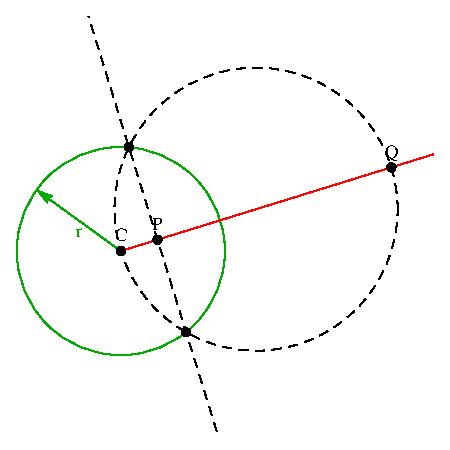
\includegraphics[width=0.5\textwidth]{figures/circ-inv}
\caption[Circle inversion]{Circle inversion with respect to the green reference circle. For a point $P$ within the reference circle the inverse $Q$ is constructed by first drawing a ray from $C$ through $P$ (red). The line normal to this ray through the point $P$ intersects the reference circle in two points. These two points together with $C$ determine a circle (dashed) which intersects the ray in the point $Q$.  The distances $CP$ and $CQ$ satisfy the relation $CP \cdot CQ = r^2$.}
\label{fig_CircInv}
\end{figure}

Coming back to the concrete map $z \mapsto \reci{z}$, it can now be interpreted the following way: Circle inversion with regard to the unit circle maps each $z \in \C$ to $\frac{z}{\abs{z}^2} = \reci{\conj{z}}$. Then reflection across the real axis (\ie complex conjugation) takes $\reci{\conj{z}}$ to $\reci{z}$. 

Summing up, all the basic types of M�bius transformations mentioned in Lemma \ref{lem_MoebiusGenerators} have a very direct geometric interpretation. Still, arbitrary M�bius transformations (especially those involving at least one inversion) are hard to describe in a similar geometric and intuitive way. Fortunately there is another characterization of M�bius transformations which is both, elegant and visually accessible.

% ---------------------------------------- Subsection: Stereographic projection
\subsection{Stereographic projection}

This section is about the great work of Douglas Arnold and Jonathan Rogness, ``M�bius transformations revealed'' \cite{arnold2008mobius}, in which the authors give a characterization of M�bius transformations in terms of stereographic projections and rigid motions of spheres 3D-space.

\todo{13}{Proof of characterization in terms of stereographic projection}


% --------------------------------------------- Subsection: Generalized circles
\subsection{Generalized circles}

\index{Generalized!circle}
From the geometric point of view M�bius transformations have the beautiful property that they preserve generalized circles. \emph{Generalized circles} are either circles (in the usual sense) or lines on the complex plane $\C$. They can also be thought of circles on the Riemann sphere (\ie the extended complex plane $\EC$ projected to the unit sphere $\UnitSphere$, see Remark~\ref{rem_RiemannSphere}), where lines on the complex plane stand in a one-to-one correspondence to circles through the point $\infty$ on the Riemann sphere. In order to give an exact definition, we follow an idea taken from \Schwerdtfeger{} and make the following considerations:

A circle with center $m \in \C$ and radius $r > 0$ can be described as the set of points $z \in \C$ for which
\begin{equation*}
\abs{z - m} = r.
\end{equation*}
This is obviously equivalent to
\begin{equation*}
\abs{z - m}^2 = (z - m) \conj{(z - m)} = r^2
\end{equation*}
and
\begin{equation}
\label{eqn_Circle}
z \conj{z} - m \conj{z} - \conj{m} z + m \conj{m} - r^2 = 0.
\end{equation}
The generalization comes into play if we multiply this last equation by a constant $A \in \R$
\begin{equation*}
A z \conj{z} - A m \conj{z} - A \conj{m} z + A m \conj{m} - A r^2 = 0
\end{equation*}
and introduce constants $B$, $C$ and $D$ appropriately such that we can write it in the form
\begin{equation}
\label{eqn_GenCircle}
A z \conj{z} + B \conj{z} + C z + D = 0.
\end{equation}
Note that $D$ is real and $B = \conj{C}$ are complex conjugates. From an equation of form (\ref{eqn_GenCircle}) we can read off the center and radius of the corresponding circle by
\begin{IEEEeqnarray}{rCl}
m &=& -\frac{B}{A}, \IEEEyessubnumber 
\label{eqn_GenCircCenter}\\
r &=& \sqrt{m \conj{m} - \frac{D}{A}} = \sqrt{\frac{BC - AD}{A^2}}. \IEEEyessubnumber 
\label{eqn_GenCircRadius}
\end{IEEEeqnarray}
Clearly we can only do so, if $A \ne 0$ and $BC - AD > 0$. 

In the case when $A = 0$, equation (\ref{eqn_GenCircle}) can be written as
\begin{equation*}
\Re{\frac{C}{\abs{C}} z} = -\frac{D}{2 \abs{C}},
\end{equation*}
which defines a line on the complex plane. We see this by considering the simpler equation $\Re{z} = -\frac{D}{2 \abs{C}}$ first (we omit the factor $\frac{C}{\abs{C}}$), which obviously defines a line parallel to the imaginary axis through the real point $-\frac{D}{2 \abs{C}}$. Then we observe that the multiplication with $\frac{C}{\abs{C}}$ just rotates this line around the origin by an angle which is given by $-\arg(C)$. 

Note that equation (\ref{eqn_GenCircle}) can also be written in matrix form:
\begin{equation*}
\rvec{\conj{z}}{1} \cdot \mat{A}{B}{C}{D} \cdot \cvec{z}{1} = 0.
\end{equation*}
If we substitute $z = u / v$, with $u,v \in \C$, $v \ne 0$ and scale by $\conj{v} \cdot v = \abs{v}^2 > 0$, we obtain the equivalent equation
\begin{equation}
\label{eqn_GenCircleMatForm}
\rvec{\conj{u}}{\conj{v}} \cdot \mat{A}{B}{C}{D} \cdot \cvec{u}{v} = 0.
\end{equation}
By introducing the convention to identify $\infty \in \EC$ with the formal quotient $u/0$, for arbitrary $u \in \C \setminus \{0\}$, equation (\ref{eqn_GenCircleMatForm}) makes sense for all $z = u/v \in \EC$. 

Finally we emphasize that the matrix in equation (\ref{eqn_GenCircleMatForm}) has a negative determinant, because of the condition $BC - AD > 0$ from above. Moreover it is a Hermitian matrix -- a notion which we will shortly recall:
\begin{definition}[Hermitian matrix]
\label{dfn_HermitianMatrix}
\index{Hermitian!matrix}
\index{Hermitian!transpose}
\index{Conjugate transpose}
Let $n > 0$ and $M \in \Mat{\C}{n}{n}$. The matrix
\begin{equation*}
\htransp{M} := \transp{\overline{M}}
\end{equation*}
obtained by complex conjugation and transposition of $M$ is called \emph{Hermitian transpose} or \emph{conjugate transpose} of $M$. If $M$ has the property $\htransp{M} = M$, it is called a \emph{Hermitian matrix}.
\end{definition}
Having now the right vocabulary and properties at hand, we can give an exact definition for generalized circles.
\begin{definition}[Generalized circle]
\index{G-circle}
\label{dfn_GenCircle}
Let $M \in \Mat{\C}{2}{2}$ be a Hermitian matrix with $\det(M) < 0$. A \emph{generalized circle}, for short \emph{g-circle}, is the set of solutions $u/v \in \EC$ with $u,v \in \C$, not both zero, to
\begin{equation}
\label{eqn_GenCircleDfn}
\rvec{\conj{u}}{\conj{v}} \cdot M \cdot \cvec{u}{v} = 0.
\end{equation}
\end{definition}

Since there should be no danger of confusion, we will from now on use the same name for a generalized circle and its corresponding Hermitian matrix (which is uniquely determined up to a nonzero real scalar factor).

\begin{remark}
Definition~\ref{dfn_GenCircle} does not depend on the choice of $u$ and $v$. If $u/v$ is a solution to (\ref{eqn_GenCircleDfn}) and $u^\prime/v^\prime = u/v$, \ie $u^\prime = \lambda u$ and $v^\prime = \lambda v$ for some $\lambda \in \C \setminus \{0\}$, then also
\begin{equation*}
\rvec{\conj{u^\prime}}{\conj{v^\prime}} \cdot M \cdot \cvec{u^\prime}{v^\prime} = \abs{\lambda}^2 \rvec{\conj{u}}{\conj{v}} \cdot M \cdot \cvec{u}{v} = 0.
\end{equation*}

Moreover we see that the point $\infty = 1/0$ lies on the g-circle $M = \smallmat{A}{B}{C}{D}$ exactly when its left upper matrix entry $A$ is zero. This is consistent with stereographic projection: The matrix entry $A$ is zero if and only if $M$ corresponds to a line on the complex plane. The image of this line under reverse stereographic projection is a circle on the Riemann sphere going through its north-pole, which we have identified with the point $\infty$.
\end{remark}

Going back to the our starting point, the equation $\abs{z - m} = r$, we can replace the equality sign `$=$' with `$<$' or `$\le$' and repeat the above considerations without any additional changes. This naturally leads to the notions of open and closed generalized disks.

\begin{definition}[Generalized disk]
\index{Generalized!disk}
\index{G-disk}
\label{dfn_GenDisk}
Let $M \in \Mat{\C}{2}{2}$ be a Hermitian matrix with $\det(M) < 0$. An \emph{open generalized disk} is the set of solutions $u/v \in \EC$, with $u,v \in \C$ -- not both zero, to
\begin{equation}
\label{eqn_GenOpenDiskDfn}
\rvec{\conj{u}}{\conj{v}} \cdot M \cdot \cvec{u}{v} < 0
\end{equation}
and a \emph{closed generalized disk} is the set of solutions $u/v \in \EC$ to
\begin{equation}
\label{eqn_GenClosedDiskDfn}
\rvec{\conj{u}}{\conj{v}} \cdot M \cdot \cvec{u}{v} \le 0.
\end{equation}
In both cases we will use the term (open/closed) \emph{g-disk} for shortness.
\end{definition}

\begin{remark}
In contrast to generalized circles, the defining matrix $M = \smallmat{A}{B}{C}{D}$ of a generalized disk is unique up to a \emph{positive} real scalar factor. Switching from $M$ to $-M$ turns the g-disk inside out while its border (the g-circle $M$) is left intact. Dependent on the sign of the left upper matrix entry $A$, we can distinguish three types of g-disks:
\begin{description}
\item[Case $A > 0$:] The g-disk corresponds to a disk in the usual sense within $\C$. Its center is given by (\ref{eqn_GenCircCenter}) and its radius by (\ref{eqn_GenCircRadius}).
\item[Case $A = 0$:] The g-disk corresponds to a half-plane of $\C$, which is obtained from the left half-plane, \ie $\Re{z} < 0$ (\resp $\le 0$), by translation by $\frac{-D}{2 \abs{C}}$ and rotation by $-\arg(C)$. The point $\infty$ is member of the generalized disk, if and only if it is closed.
\item[Case $A < 0$:] The open g-disk $M$ corresponds to the set complement (within $\EC$) of the closed g-disk $-M$ (discussed in the first case, $A > 0$). Accordingly, the closed g-disk $M$ is the complement of the open g-disk $-M$. Open and closed g-disks with $A < 0$ contain the point  $\infty$.
\end{description}
\end{remark}

It is now easy to show that g-circles and g-disks are preserved under M�bius transformations.

\begin{theorem}
\label{thm_MoebiusGenCircle}
Let $\phi$ be a M�bius transformation and $M \in \Mat{\C}{2}{2}$ be a Hermitian matrix with $\det(M) < 0$. The image of the g-circle (\resp open/closed g-disk) $M$ under the M�bius transformation $\phi$ corresponding to the matrix $P \in \GL{\C}$ is the g-circle (\resp open/closed g-disk)
\begin{equation}
\label{eqn_GDiskTransform}
\htransp{(\inv{P})} \cdot M \cdot \inv{P}.
\end{equation}
\end{theorem}
\begin{proof}
Let us write $P = \smallmat{a}{b}{c}{d}$, such that the corresponding M�bius transformation $\phi$ has the form
\begin{equation*}
\phi\left(\frac{u}{v}\right) = \frac{a u + b v}{c u + d v}.
\end{equation*}
Define $u^\prime := a u + b v$ and $v^\prime := c u + d v$. We need to show that
\begin{equation*}
\rvec{\conj{u}}{\conj{v}} \cdot M \cdot \cvec{u}{v} 
\ \left\{\ \begin{matrix} = 0 \\ < 0\\ \le 0 \end{matrix}\right.
\end{equation*}
if and only if
\begin{equation*}
\rvec{\conj{u^\prime}}{\conj{v^\prime}} \cdot \htransp{(\inv{P})} \cdot M \cdot \inv{P} \cdot \cvec{u^\prime}{v^\prime} 
\ \left\{\ \begin{matrix} = 0\phantom{.} \\ < 0\phantom{.}\\ \le 0. \end{matrix}\right.
\end{equation*}
But this follows immediately from
\begin{equation*}
P \cdot \cvec{u}{v} = \cvec{a u + b v}{c u + d v} = \cvec{u^\prime}{v^\prime}.\qedhere
\end{equation*}
\end{proof}




% ------------------------------------------------------ CHAPTER: MODULAR GROUP
\chapter{The modular group}

% ---------------------------------------------- Section: Generators, Relations
In this chapter and also later, we adopt the notation of \Schoeneberg{}.

\begin{definition}[Modular transformation]
\label{dfn_ModularGroup}
\index{Modular!group}
\index{Modular!transformation}
\index{Inhomogeneous!modular transformation}
A M�bius transformation $A$ of the form
\begin{equation*}
A(z) = \moebius{a}{b}{c}{d}{z},\quad a,b,c,d \in \Z,\quad ad - bc = 1
\end{equation*}
is called \emph{(inhomogeneous) modular transformation}.
\end{definition}

\begin{theorem}[Modular group]
\label{thm_ModularGroup}
\index{Modular!group}
The set of modular transformations forms a subgroup of the group of M�bius transformations and can be identified with the projective special linear group $\PSL{\Z}$. This group is called the \emph{modular group}. %and is denoted by $\ModGrp$.
\end{theorem}
\begin{proof}
The proof is very similar to that of Theorem \ref{thm_MoebiusGroup}. The only thing which has to be changed is the homomorphism $\pi$ defined in (\ref{eqn_homPi}). Its domain now is $\SL{\Z}$, the group of 2-by-2 matrices over $\Z$ with determinant 1, rather than $\GL{\C}$ (or $\SL{\C}$). It follows by the first isomorphism theorem (Theorem~\ref{thm_FirstIsoThm}), that the modular group is isomorphic to $\SL{\Z} / \ker(\pi) \cong \PSL{\Z}$. The fact that the modular group is a subgroup of the group of M�bius transformations is now also evident, since $\PSL{\Z} \le \PSL{\C} \cong \PGL{\C}$ (see Example~\ref{ex_ProjAndGenLinGrp}).
\end{proof}

\begin{remark}
\index{Inhomogeneous!modular transformation}
\index{Homogeneous!modular transformation}
\index{Modular!transformation}
The elements of $\SL{\Z}$ are often called \emph{homogeneous modular transformations}, whereas the transformations of $\PSL{\Z}$ are called \emph{inhomogeneous transformations}. Strictly seen, an inhomogeneous transformation has to be denoted as $[M]_{\sim}$, which is the equivalence class in $\PSL{\Z}$ of a matrix $M \in \SL{\Z}$. It is clear, that $[M]_{\sim}$ is nothing but the set $\{\pm M\}$ and again for easier notation, we will from now on simply write either $M$ or $-M$ instead of $[M]_{\sim}$. Additionally we will denote equivalence of matrices by $\sim$, \ie if $\lambda = \pm 1$, then $M \sim \lambda M$.
\end{remark}

\section{Generators and relations}
\label{sec_ModularGroupGenRel}

In group theory it is an important question, which presentations (in view of Definition~\ref{dfn_GrpConstructGenRel}) can be given for a fixed group $G$. This section is devoted to the investigation of this question in the case of the modular group.

Before we start, we introduce the following notation for rounding real numbers to integers:

\begin{definition}[Rounding functions]
\label{dfn_RoundingFunctions}
\index{Floor function}
\index{Ceiling function}
\index{nint (Nearest integer function)}
For $x \in \R$, the \emph{floor function} $\floor{x}$, the \emph{ceiling function} $\ceil{x}$ and the \emph{nearest integer function} $\nint{x}$ are defined as
\begin{eqnarray}
\label{eqn_defFloor}
\floor{x} &:=& \max \setdef{k \in \Z}{k \le x},\\
\label{eqn_defCeil}
\ceil{x} &:=& \min \setdef{k \in \Z}{k \ge x},\\
\label{eqn_defNint}
\nint{x} &:=& \sgn{x} \ceil{\abs{x} - \reci{2}}.
\end{eqnarray}
\end{definition}

\begin{remark}
It is quite common to define the nearest integer function such that half-integers are always rounded to even numbers. For our purposes this makes no essential difference and we prefer the above definition -- rounding half-integers toward zero -- for its simpler closed form.
\end{remark}

Additionally we will need three modular transformations very frequently from now on:

\begin{definition}
\label{dfn_ModGrpBasicTransforms}
We denote by $U$, $T$ and $R$ the following modular transformations:
\begin{IEEEeqnarray*}{RL}
U: & z \mapsto z + 1 \\
T: & z \mapsto -\reci{z} \\
R = TU: & z \mapsto -\reci{z + 1}
\end{IEEEeqnarray*}
\end{definition}

\begin{remark}
Unfortunately in literature there is no consensus on the notation of these transformations. We use the notation of \Schoeneberg{} here, but other notations are frequent. For example in \Klein{}, the symbol $S$ is used instead of $U$ and in other literature as well as on Wikipedia, additionally the roles of $S$ and $T$ are swapped.
\end{remark}

\begin{theorem}
\label{thm_ModGrpTUGen}
The modular group is generated by the elements $U: z \mapsto z+1$ and $T: z \mapsto -\reci{z}$. 
\end{theorem}
\begin{proof}
Let $A: z \mapsto \moebius{a}{b}{c}{d}{z}$ be an arbitrary modular transformation. Our goal is to show that $A$ can be written as product of the transformations $U$ and $T$. For this purpose it is more convenient to view these transformations as elements of $\PSL{\Z}$, namely
\begin{equation*}
A = \mat{a}{b}{c}{d}, \quad U = \mat{1}{1}{0}{1}, \quad T = \mat{0}{-1}{1}{\phantom{+}0}.
\end{equation*}

Let's first consider the two special cases, when $a$ or $c$ are zero. If $a=0$, it follows from $ad - bc = 1$, that $-b = c = \pm 1$. Therefore we have (equivalence of matrices is again denoted by $\sim$)
\begin{equation*}
A \sim c A = \mat{0}{-1}{1}{c d} = TU^{c d}.
\end{equation*}
Similarly, $c = 0$ gives $a = d = \pm 1$ and
\begin{equation*}
A \sim a A = \mat{1}{a b}{0}{1} = U^{a b}.
\end{equation*}
In the more general case, when $a$ and $c$ are both nonzero, $ad - bc = 1$ implies that $a$ and $c$ are coprime and the Euclidean algorithm therefore yields a finite sequence of equations
\begin{eqnarray*}
      a &=& q_0 \cdot c\phantom{_0} + r_1 \\
      c &=& q_1 \cdot r_1 + r_2 \\
    r_1 &=& q_2 \cdot r_2 + r_3 \\
        &\vdots& \\
r_{n-1} &=& q_n \cdot r_n + r_{n+1}\\
        &=& q_n \cdot (\pm 1) + 0.
\end{eqnarray*}
Note that the quotients $q_j$ and the remainders $r_j$ depend on the choice of the rounding method for integer division (this will be discussed in more detail in Remark~\ref{rem_EuclideanAlgorithmRounding}).

We can use the above sequence of equations to reduce the Matrix $A$ by successively multiplying powers of $U$ and $T$ from the left. Just note that multiplication with $U^k$ adds $k$ times the second row to the first row, whereas $T$ swaps the rows and changes the sign of one arbitrary row.\footnote{This freedom of choice is again due to the fact that the matrices $M$ and $-M$ represent the same element in $\PSL{\Z}$.} If we concentrate only on the first column of $A$ and apply the first few transformations
\begin{equation*}
\cvec{a}{c}                           \overset{U^{-q_0}}{\longmapsto}
\cvec{r_1}{c\phantom{_1}}             \overset{T}{\mapsto} 
\cvec{\phantom{+}c\phantom{_1}}{-r_1} \overset{U^{q_1}}{\longmapsto}
\cvec{\phantom{+}r_2}{-r_1}           \overset{T}{\mapsto} 
\cvec{r_1}{r_2}                       \overset{U^{-q_2}}{\longmapsto}
\cvec{r_3}{r_2}                       \overset{T}{\mapsto}
\cvec{\phantom{+}r_2}{-r_3}           \mapsto \dots,
\end{equation*}
we soon recognize the general mapping rule, which is
\begin{IEEEeqnarray*}{rCll}
\cvec{\phantom{+}r_{j-1}}{\phantom{+}r_{j\phantom{+0}}} 
& \overset{TU^{-q_j}}{\longmapsto}
& \cvec{\phantom{+}r_{j\phantom{+0}}}{-r_{j+1}}
& \quad \text{for even } j \text{ and}\\
\cvec{\phantom{+}r_{j-1}}{-r_{j\phantom{+0}}}
& \overset{TU^{q_j}}{\longmapsto}
& \cvec{\phantom{+}r_{j\phantom{+0}}}{\phantom{+}r_{j+1}} 
& \quad \text{for odd } j.
\end{IEEEeqnarray*}
When we set $r_{-1} := a$ and $r_0 := c$, this rule is applicable for $0 \le j \le n$. Obviously the described procedure ends with
\begin{equation*}
\cdots \overset{T}{\mapsto}
\cvec{\phantom{+}r_{n\phantom{+0}}}{\pm r_{n+1}} = \cvec{\pm 1}{\phantom{\pm}0}.
\end{equation*} 
Because we know the first column of the resulting matrix and its determinant, which is 1, we can conclude that for some $k \in \Z$ it must have the form
\begin{equation*}
\pm\mat{1}{k}{0}{1} \sim U^k.
\end{equation*}
By setting $e_n := (-1)^{n} q_n$ we therefore have 
\begin{equation*}
TU^{-e_n} TU^{-e_{n-1}} \cdots TU^{-e_1}TU^{-e_0} A = U^k,
\end{equation*}
or equivalently -- noting that $\inv{T} = T$, 
\begin{equation*}
A = U^{e_0} TU^{e_1} \cdots TU^{e_{n-1}} TU^{e_n} T U^k,
\end{equation*}
which gives the desired representation of $A$ in terms of $U$ and $T$ in the case when $a$ and $c$ are both nonzero.
\end{proof}

\begin{corollary}
\label{cor_SLZandPSLZGen}
The special linear group $\SL{\Z}$ is generated by the matrices $U = \smallmat{1}{1}{0}{1}$ and $T = \smallmat{0}{-1}{1}{\phantom{-}0}$. The projective special linear group $\PSL{\Z}$ is generated by the equivalence classes ${}_\pm U$ and ${}_\pm T$.\footnote{Here we use the notation ${}_\pm M := M_\sim = \{\pm M\} \in \PSL{\Z}$ for clearer distinction between the matrix $M \in \SL{\Z}$ and its corresponding equivalence class in $\PSL{\Z}$.}
\end{corollary}
\begin{proof}
The second statement is obviously a simple reformulation of Theorem~\ref{thm_ModGrpTUGen}. As a consequence, for every matrix $M \in \SL{\Z}$ there exists a product of matrices $T$ and $U$ which evaluates to either $M$ or $-M$. In the case when the product is $-M$, multiplication with the additional factor $T^2 = -\smallmat{1}{0}{0}{1}$ gives a product for $M$. This also proves the first statement.
\end{proof}

It is worth formulating the algorithm used in the proof of Theorem~\ref{thm_ModGrpTUGen} explicitly in the following corollary.
\begin{corollary}[The $T$-$U$ algorithm]
\label{cor_ModGrpTUAlg}
An arbitrary modular transformation $A: z \mapsto \moebius{a}{b}{c}{d}{z}$ can be represented as product of the transformations $U: z \mapsto z+1$ and $T : z \mapsto -\reci{z}$, by performing the following steps:
\begin{enumerate}
%\item If $a = 0$, then $A = TU^{c d}$ and if $c = 0$, then $A = U^{a b}$ and we are done. Otherwise, continue with \ref{itm_ModGrpTUAlgStart}.
\item \label{itm_ModGrpTUAlgStart} Apply the Euclidean algorithm to $a$ and $c$ with the first division being $a = q_0 \cdot c + r_1$ ($q_0$ may be $\le 0$) and let $n$ be the number of the  last division (start counting from 0). Call the arising quotients $q_0,q_1,\dots,q_n$. 

Note that if $a = 0$, the Euclidean algorithm will terminate after the first iteration, yielding the one-element quotient sequence $q_0 = 0$ and $n = 0$. If $c = 0$, it will terminate immediately, giving an empty sequence of quotients and $n = -1$.
\item For $j \in \{0,1,\dots,n\}$ set $e_j := (-1)^j q_j$.
\item Calculate the matrix product $TU^{-e_n} TU^{-e_{n-1}} \cdots TU^{-e_1}TU^{-e_0} A$ and multiply by $\pm 1$ in order to obtain a representation with positive diagonal elements. Read off the right-upper entry and call it $k$.
\end{enumerate}
The transformation $A$ can now be written as
\begin{equation}
\label{eqn_ModGrpTUAlg}
A = U^{e_0} TU^{e_1} \cdots TU^{e_{n-1}} TU^{e_n} T U^k.
\end{equation}
\end{corollary}

\begin{remark}
\label{rem_EuclideanAlgorithmRounding}
The product representation (\ref{eqn_ModGrpTUAlg}) is not unique. In fact there is quite some freedom of choice for the quotients $q_0, q_1, \ldots, q_n$ in the above $T$-$U$ algorithm. With the convention $r_{-1} := a$ and $r_0 := c$, one usually sets $q_j := \floor{\frac{r_{j-1}}{r_j}}$ for $j \ge 0$. The remainders, which are determined by 
\begin{equation}
\label{eqn_EuclideanAlgorithmLine}
r_{j+1} = r_{j-1} - q_j \cdot r_j \quad \text{for } j \ge 0,
\end{equation}
are then all nonnegative and form a strictly monotonic decreasing sequence,
\begin{equation*}
r_1 > r_2 > \ldots > r_n > r_{n+1} = 0.
\end{equation*}
All quotients, with the possible exception of $q_0$, are positive. In contrast to that, if we choose for each $j$ an arbitrary rounding direction (up- or downwards) and set $q_j$ to either $\floor{\frac{r_{j-1}}{r_j}}$ or $\ceil{\frac{r_{j-1}}{r_j}}$, then in general also negative remainders (and consequently negative quotients) will occur. Still, the absolute values of the remainders form a strictly monotonic decreasing sequence,
\begin{equation*}
\abs{r_1} > \abs{r_2} > \ldots > \abs{r_n} > \abs{r_{n+1}} = 0.
\end{equation*}
Therefore the Euclidean algorithm terminates and yields a correct result.\footnote{The determined greatest common divisor is possibly negative, which is still admissible, because if $d$ is a greatest common divisor of $n,m \in \Z$, \ie $\forall d^\prime \in \Z: (d^\prime \mid n,m \Rightarrow d^\prime \mid d)$, then also $-d$ is.} Depending on the choice of the rounding directions we will in general obtain different product representations of $A$. Not only this, we can even go one step further and violate the constraint $\abs{r_j} > \abs{r_{j+1}}$ for a finite number of indices $j$ by choosing a completely random $q_j \in \Z$. As long as the remainders are calculated through (\ref{eqn_EuclideanAlgorithmLine}), all product representations obtained in this way are correct.
\end{remark}
\begin{example}
\label{ex_TUWordRounding}
Consider the modular transformation $A \in \PSL{\Z}$ given by
\begin{equation*}
A = \mat{13}{5}{-8}{-3}.
\end{equation*}
Applying algorithm~\ref{cor_ModGrpTUAlg} and setting $q_j := \floor{\frac{r_{j-1}}{r_j}}$ for all $j$ yields the product representation
\begin{equation*}
A = U^{-2} TU^{-2} TU^1 TU^{-2} T.
\end{equation*}
In contrast to that, setting $q_j := \ceil{\frac{r_{j-1}}{r_j}}$ in each step leads to
\begin{equation*}
A = U^{-1} TU^1 TU^{-1} TU^1 TU^{-2} T.
\end{equation*}
Last but not least, always rounding to the nearest integer, that is setting $q_j := \nint{\frac{r_{j-1}}{r_j}}$, gives the shortest representation:
\begin{equation*}
A = U^{-2} TU^{-3} TU^{-3} T.
\end{equation*}
Note that this is true in general: Rounding to the nearest integer always leads to a product representation with minimal number of factors $T$ and $U^k$. According to \Ore{}, already Leopold Kronecker has shown that among all variants of the Euclidean algorithm, the one which uses rounding to the nearest integer requires a minimum number of steps. We will come back to this fact once more in  Remark~\ref{rem_TUAlgConFrac}.
\end{example}

We have now seen that $T$ and $U$ generate the modular group and different product representations for a given modular transformation $A$ can be found using the above $T$-$U$ algorithm. Of course the questions arises, which  relations (in sense of Definition~\ref{dfn_GrpConstructGenRel}) lie behind the ambiguity of these product representations. For example, it is easy to see that $T^2 = 1$ and $(TU)^3 = 1$ are relations which are satisfied by $T$ and $U$. It is the goal of the following paragraphs to show that these two relations are in fact the only ones in the sense that all other relations are derived from these. We will do this by proving the following theorem:

\begin{theorem}[Unique $T$-$R$ representation]
\label{thm_ModGrpTRProd}
Let $T: z \mapsto -\reci{z}$ and $R = TU: z \mapsto -\reci{z+1}$. Every modular transformation $A \in \PSL{\Z}$ can be written uniquely in the form
\begin{equation}
\label{eqn_ModGrpTRProd}
A = R^{k_1} T R^{k_2} T \cdots R^{k_{n-1}} T R^{k_n} 
\end{equation}
with $n \in \N$, $k_2,\dots,k_{n-1} \in \{\pm 1\}$ and $k_1, k_n \in \{0, \pm 1\}$.
\end{theorem}

From the uniqueness of the product representation (\ref{eqn_ModGrpTRProd}) it follows that we have in fact a \emph{presentation} of the modular group in the sense of Definition~\ref{dfn_GrpConstructGenRel}:

\begin{corollary}[$T$-$R$ presentation]
\label{cor_ModGrpPresentation}
The modular group is generated by the elements $T: z \mapsto -\reci{z}$ and $R: z \mapsto -\reci{z+1}$ and can be presented as
\begin{equation}
\label{eqn_ModGrpPresentation}
\PSL{\Z} \cong \presentation{T,R}{T^2 = R^3 = 1}.
\end{equation}
Therefore $\PSL{\Z}$ is isomorphic to the free product of a cyclic group of order 2 and a cyclic group of order 3.
\end{corollary}
\begin{proof}
It is easy to see that the relations $T^2 = R^3 = 1$ are indeed satisfied:
\begin{eqnarray*}
T^2 &=& \mat{0}{-1}{1}{\phantom{-}0}^2 = \mat{-1}{\phantom{-}0}{\phantom{-}0}{-1} \sim \mat{1}{0}{0}{1}, \\
R^3 &=& \mat{0}{-1}{1}{\phantom{+}1}^3 = \mat{-1}{\phantom{-}0}{\phantom{-}0}{-1} \sim \mat{1}{0}{0}{1}.
\end{eqnarray*}
Moreover the elements of $\presentation{T,R}{T^2 = R^3 = 1}$ are precisely the group words of the form~(\ref{eqn_ModGrpTRProd}), as we have seen in Examples~\ref{ex_RTGroup} and \ref{ex_RTFreeProd}.
\end{proof}

Before we turn to the proof of Theorem~\ref{thm_ModGrpTRProd}, we first make one helpful definition and study its consequences.

\begin{definition}
\label{dfn_trsPredicates}
For a modular transformation $A: z \mapsto \moebius{a}{b}{c}{d}{z}$, we define the predicates $t$, $r$ and $s$ as well as a ``grading'' $n$:
\begin{IEEEeqnarray}{rCcCc}
\label{eqn_tpred}
t(A) &:\quad& ac \ge 0       &\quad\land\quad& bd \ge 0 \\
\label{eqn_rpred}
r(A) &:\quad& a^2 + ac \le 0 &\quad\land\quad& b^2 + bd \le 0 \\
\label{eqn_spred}
s(A) &:\quad& c^2 + ac \le 0 &\quad\land\quad& d^2 + bd \le 0
\end{IEEEeqnarray}
\begin{equation}
\label{eqn_grading}
n(A) := a^2 + b^2 + c^2 + d^2.
\end{equation}
\end{definition}

Note that $t$, $r$, $s$ and $n$ are well-defined, since they do not change their value if we switch from the matrix $A \in \PSL{\Z}$ to the equivalent matrix $-A$, \eg $t(A) \Leftrightarrow t(-A)$ and $n(A) = n(-A)$. Moreover the predicates $t$, $r$, and $s$ partition the elements of the modular group into three classes:

\begin{lemma}
\label{lem_trsPartition}
Let $A: z \mapsto \moebius{a}{b}{c}{d}{z}$ be an arbitrary modular transformation. Then one and only one of the predicates $t(A)$, $r(A)$ and $s(A)$ is satisfied.
\end{lemma}
\begin{proof}
We start by considering the two easiest cases first: If $A$ is the identity transformation or $A = T$, we have $t(A)$, $\lnot s(A)$ and $\lnot r(A)$.

For all other cases, we note that at least three of the coefficients $a,b,c,d$ are nonzero. Therefore, if \label{err_SuperfluousOne} the predicate $t(A)$ is satisfied, then at least one of the two inequalities involved is \emph{strictly} fulfilled, \ie $ac > 0$ or $bd > 0$. Having this said, it is easy to see that $t(A) \Rightarrow \lnot r(A) \land \lnot s(A)$. Thus it remains to show 
\begin{equation*}
\lnot t(A) \Rightarrow r(A) \lxor s(A),
\end{equation*}
for all transformations with at least three nonzero coefficients (here, $\lxor$ denotes logical exclusive or). If $t(A)$ is false, we have $ac < 0$ or $bd < 0$. Since both cases are completely symmetric, we may assume without restriction that $ac < 0$. Note that $ac < 0$ and $ad - bc = 1$ implies $bd \le 0$ because otherwise if $bd > 0$, both nonzero terms $ad$ and $bc$ would have different  signs and their difference could not be 1. We conclude the proof by distinguishing three cases:
\begin{description}
\item[Case $a^2 < c^2$:] From $ac < 0$ it follows that $a^2 + ac < 0\ (i)$ and $c^2 + ac > 0\ (ii)$. Additionally, from $ad - bc = 1$ we can conclude that $b^2 \le d^2$, because otherwise $\abs{ad}$ would differ from $\abs{bc}$ by more than 1. Therefore we also have $b^2 + bd \le 0\ (iii)$. Taking these pieces together, we have $(ii) \Rightarrow \lnot s(A)$ and $(i) \land (iii) \Rightarrow r(A)$.
\item[Case $a^2 > c^2$:] This case is complementary to the first one: Because of $ac < 0$ we have $a^2 + ac > 0\ (i)$ and $c^2 + ac < 0\ (ii)$. The equation $ad - bc = 1$ here implies $b^2 \ge d^2$ and $d^2 + bd \le 0\ (iii)$. Thus we have $(i) \Rightarrow \lnot r(A)$ and $(ii) \land (iii) \Rightarrow s(A)$.
\item[Case $a^2 = c^2$:] Note that this case is only possible with $a = -c = \pm 1$ (as $a$ and $c$ are coprime). Hence we have $a^2 + ac = c^2 + ac = 0$. However, $ad - bc = 1$ implies $b^2 \ne d^2$ and therefore we have $b^2 + bd \le 0 \lxor d^2 + bd \le 0$. So, also in this case $r(A) \lxor s(A)$ holds.\qedhere
\end{description}
\end{proof}

We have not yet seen the real benefit and meaning of the predicates $t$, $r$ and $s$. The following lemma will imply that they do nothing but indicate the leftmost symbol in the unique $T$-$R$ product representation (\ref{eqn_ModGrpTRProd}) of $A$. To be precise, if we denote this leftmost symbol by $\alpha(A)$, we will see that $t(A) \Leftrightarrow \alpha(A) = T$, $r(A) \Leftrightarrow \alpha(A) = R$ and $s(A) \Leftrightarrow \alpha(A) = \inv{R}$. Moreover we will show that the grading $n(A)$ grows monotonically with the number of symbols $R$ and $\inv{R}$ in the product representation of $A$.

\begin{lemma}
\label{lem_trsnRelations}
The predicates $t$, $r$, $s$ and the grading $n$ satisfy the following relations:
\begin{enumerate}[\qquad(i)]
\item \label{itm_trsPropA}
$t(A) \Leftrightarrow r(RA) \Leftrightarrow s(\inv{R}A)$

\item \label{itm_trsPropB}
$t(A) \land t(TA) \Leftrightarrow A \in \{1,T\}$

\item \label{itm_trsPropC} 
$n(A) = n(TA)$

\item \label{itm_trsPropD}
$t(A) \Rightarrow n(A) < n(RA)\ \land\ n(A) < n(\inv{R}A)$

\end{enumerate}
\end{lemma}
\begin{proof}
For a better overview, we first write out the matrices corresponding to $TA$, $RA$ and $\inv{R}A$. Since $A = \smallmat{a}{b}{c}{d}$, $T = \smallmat{0}{-1}{1}{\phantom{-}0}$, $R = \smallmat{0}{-1}{1}{\phantom{+}1}$ and $\inv{R} = \smallmat{\phantom{+}1}{1}{-1}{0}$ these are:
\begin{equation*}
TA = \mat{-c}{-d}{\phantom{+}a}{\phantom{+}b},\quad RA = \mat{-c}{-d}{a+c}{b+d},\quad
\inv{R}A = \mat{a+c}{b+d}{-a}{-b}.
\end{equation*}
\begin{description}
\item[ad (\ref{itm_trsPropA}):] This is shown easily via two simple calculations:
\begin{IEEEeqnarray*}{rClCl}
r(RA)
&\Leftrightarrow& c^2 - c(a+c) \le 0 \land d^2 - d(b+d) \le 0 & &  \\
&\Leftrightarrow& ac \ge 0 \land bd \ge 0 &\Leftrightarrow& t(A) \\
s(\inv{R}A)
&\Leftrightarrow& a^2 - a(a+c) \le 0 \land b^2 - b(b+d) \le 0 & & \\
&\Leftrightarrow& ac \ge 0 \land bd \ge 0 &\Leftrightarrow& t(A)
\end{IEEEeqnarray*}
\item[ad (\ref{itm_trsPropB}):] It is immediate to see that $t(A) \land t(TA)$ is equivalent to $ac = bd = 0$. Clearly, 1 and $T$ are the only two transformations satisfying this condition.
\item[ad (\ref{itm_trsPropC}):] $n(A) = n(TA)$ is trivial.
\item[ad (\ref{itm_trsPropD}):] Note that $ad - bc = 1$ implies that at least one of the numbers $a$ and $b$ (resp.\ $c$ and $d$) is nonzero. Moreover, $t(A) \Rightarrow ac \ge 0 \land bd \ge 0$, and thus we have
\begin{IEEEeqnarray*}{+rCl+x*}
n(RA) - n(A)       &=& c^2 + 2ac + d^2 + 2bd > 0 \quad \text{and}\\
n(\inv{R}A) - n(A) &=& a^2 + 2ac + b^2 + 2bd > 0.&\qedhere
\end{IEEEeqnarray*}
\end{description}
\end{proof}

We can now formulate an algorithm which yields a product representation of any arbitrary modular transformation in terms of the generators $R$ and $T$.

\begin{theorem}[The $T$-$R$ algorithm]
\label{thm_ModGrpTRAlg}
For a modular transformation $A: z \mapsto \moebius{a}{b}{c}{d}{z}$, a product representation of the form (\ref{eqn_ModGrpTRProd}) can be found by performing the following steps:
\begin{enumerate}
\item Start with $k := 0$ and set $A_0 := A$.

\item If $A_k = 1$ go to step \ref{itm_ModGrpTRAlgFin}.
\label{itm_ModGrpTRAlgLoop}

\item Define $M_k$ as follows:
\label{itm_ModGrpTRAlgMDfn}
\begin{equation*}
t(A_k) \Rightarrow M_k := T,\quad
r(A_k) \Rightarrow M_k := R,\quad
s(A_k) \Rightarrow M_k := \inv{R}.
\end{equation*}

\item Set $A_{k+1} := M_k^{-1} A_k$, increment $k$ by one and continue with step \ref{itm_ModGrpTRAlgLoop}.
\label{itm_ModGrpTRAlgADfn}

\item If $k = 0$, then $A = 1$, which is the empty product. Otherwise, the desired product representation is $A = M_0 M_1 \cdots M_{k-1}$.
\label{itm_ModGrpTRAlgFin}
\end{enumerate}
\end{theorem}
\begin{proof}Note that by Lemma~\ref{lem_trsPartition} the rule for the definition of the transformations $M_k$ from step \ref{itm_ModGrpTRAlgMDfn} is unambiguous and the described algorithm therefore yields a unique sequence of equations 
\begin{eqnarray*}
A_1 &=& M_0^{-1} A_0\\
A_2 &=& M_1^{-1} A_1\\
A_3 &=& M_2^{-1} A_2\\
    &\vdots&
\end{eqnarray*}
The relations (\ref{itm_trsPropA}) and (\ref{itm_trsPropB}) of Lemma~\ref{lem_trsnRelations} guarantee that for every pair of subsequent transformations $M_k$, $M_{k+1}$, one of them is $T$ and the other is either $R$ or $\inv{R}$. Additionally, the relations (\ref{itm_trsPropC}) and (\ref{itm_trsPropD}) imply $n(A_k) > n(A_{k+2})$. Since $n(1) = n(T) = 2$ is a lower bound for $n(A_k)$, the described procedure must terminate after a finite number $m$ of iterations and the product $A = M_0 M_1 \cdots M_{m-1}$ is indeed of the desired form (\ref{eqn_ModGrpTRProd}).
\end{proof}

Now have all tools in hand for the proof of Theorem~\ref{thm_ModGrpTRProd}. Note that two alternative proofs can be found in \Schoeneberg{}, �4 and in \Klein{}, p.\ 452ff.\footnote{Volume 1, part 2, chapter 9, �1.} 

\begin{proof}[Proof of Theorem \ref{thm_ModGrpTRProd}]
Let $A: z \mapsto \moebius{a}{b}{c}{d}{z}$ be an arbitrary modular transformation. The existence of a product representation of the form (\ref{eqn_ModGrpTRProd}) is ensured by the above $T$-$R$ algorithm. 

In order to prove also its uniqueness, it is sufficient to show that the identity map has a unique product representation (namely the empty product). From the relations (\ref{itm_trsPropC}) and (\ref{itm_trsPropD}) of Lemma~\ref{lem_trsnRelations} we see that any product $P$ of the form (\ref{eqn_ModGrpTRProd}) containing at least one factor $R$ or $\inv{R}$ has a grading $n(P) > n(1) = 2$ and therefore $P \ne 1$. The only products which are free of factors $R$ and $\inv{R}$ are T and the empty product. Since $T \ne 1$, the identity map can indeed only be represented by the empty product. \qedhere
\end{proof}

\begin{example}
We apply the algorithm of Theorem~\ref{thm_ModGrpTRAlg} to the modular transformation from Example~\ref{ex_TUWordRounding},
\begin{equation*}
A = \mat{13}{5}{-8}{-3}.
\end{equation*}
After substitution of $\inv{R} = R^2$, we end up with the $R$-$T$ product representation
\begin{equation*}
A = R^2 T R^1 T R^2 T R^1 T R^2 T R^2.
\end{equation*}
Note that alternatively we could just as well have started with one of the $T$-$U$ product representations of Example~\ref{ex_TUWordRounding} and substitute $U = TR$ and $\inv{U} = R^2 T$. Cancellation of terms $T^2 = 1$ and $R^3 = 1$ then would, by Theorem~\ref{thm_ModGrpTRProd}, necessarily lead to the same $T$-$R$ product representation.
\end{example}

\begin{remark}
\label{rem_ModGrpTRAlg}
We conclude this section with the final remark that the $T$-$R$ algorithm successively reduces a given matrix $A \in \PSL{\Z}$ by multiplication from the left with $T$, $R$ or $\inv{R}$. Of course, by using a dual approach also multiplication from the right can be used. All we have to do in order to adapt the algorithm appropriately is to substitute the predicates $t$, $r$, $s$ by predicates $t^{\prime}$, $r^{\prime}$, $s^{\prime}$ and to change the definition in step \ref{itm_ModGrpTRAlgADfn} from $A_{k+1} := M_k^{-1} A_k$ to $A_{k+1} := A_k M_k^{-1}$. But how do the predicates $t^{\prime}$, $r^{\prime}$ and $s^{\prime}$ have to be defined?

For this consideration we denote the leftmost symbol in the $R$-$T$ product representation (\ref{eqn_ModGrpTRProd}) of $A$ by $\alpha(A)$ and the rightmost symbol by $\omega(A)$. In the case of the empty product, we define $\alpha(1) := \omega(1) := T$. We have already seen that $t(A) \Leftrightarrow \alpha(A) = T$, $r(A) \Leftrightarrow \alpha(A) = R$ and $s(A) \Leftrightarrow \alpha(A) = \inv{R}$. In correspondence to that, we see that we have to define 
\begin{IEEEeqnarray*}{RrClCrClCc}
t^{\prime}(A):\quad& \omega(A) &=& T 
              &\quad\Leftrightarrow\quad& \alpha(\inv{A}) &=& T
              &\quad\Leftrightarrow\quad& t(\inv{A}), \\
r^{\prime}(A):\quad& \omega(A) &=& R 
              &\quad\Leftrightarrow\quad& \alpha(\inv{A}) &=& \inv{R}
              &\quad\Leftrightarrow\quad& s(\inv{A}), \\
s^{\prime}(A):\quad& \omega(A) &=& \inv{R}
              &\quad\Leftrightarrow\quad& \alpha(\inv{A}) &=& R
              &\quad\Leftrightarrow\quad& r(\inv{A}).
\end{IEEEeqnarray*}
Written out explicitly, this gives for a matrix $A = \smallmat{a}{b}{c}{d} \in \PSL{\Z}$:
\begin{IEEEeqnarray}{rCcCc}
\label{eqn_trpred}
t^{\prime}(A) &:\quad& ab \le 0       &\quad\land\quad& cd \le 0 \\
\label{eqn_rrpred}
r^{\prime}(A) &:\quad& a^2 - ab \le 0 &\quad\land\quad& c^2 - cd \le 0 \\
\label{eqn_srpred}
s^{\prime}(A) &:\quad& b^2 - ab \le 0 &\quad\land\quad& d^2 - cd \le 0
\end{IEEEeqnarray}
Note that also the Lemmas \ref{lem_trsPartition} and \ref{lem_trsnRelations} remain valid, if the predicates $t$, $r$, $s$ are substitued by $t^{\prime}$, $r^{\prime}$, $s^{\prime}$ and the order of matrix multiplication is reversed (\ie $RA$, $TA$, \dots\ have to be replaced by $AR$, $AT$, \dots).
\end{remark}



% ------------------------------------------------ Section: Fundamental Domains 
\section{Fundamental sets and regions}

We have seen in Remark~\ref{rem_NatureMoebius} that considering M�bius transformations as meromorphic functions $\EC \to \EC$ very naturally induces a group action of $\PGL{\C}$ on $\EC$. Clearly this group action is also given for any subgroup of $\PGL{\C}$ and in particular for the modular group: For $A = \smallmat{a}{b}{c}{d} \in \PSL{\Z}$ the group action is given by
\begin{equation}
\label{eqn_ModGrpAction}
Az := \moebius{a}{b}{c}{d}{z}.
\end{equation}

As usual we call two points $z, w \in \EC$ \emph{equivalent}, in symbols $z \sim w$, if there is a transformation $A \in \PSL{\Z}$ such that $Az = w$. We are now interested in subsets of $\EC$ containing exactly one point from each equivalence class of the relation $\sim$:

\begin{definition}[Fundamental set]
\label{dfn_FundamentalSet}
\index{Fundamental!set}
Let $G$ be a group acting on the set $\mathcal{S}$. Denote equivalence of points in $\mathcal{S}$ under $G$ by $\sim$, as in (\ref{eqn_GroupActionEquivalence}). A subset $\FunSet \subseteq \mathcal{S}$ is called a \emph{fundamental set} with respect to the group action of $G$ on $\mathcal{S}$, if $\FunSet$ contains exactly one point from each orbit $Gx = [x]_\sim$, \ie the map $\FunSet \to \mathcal{S}/\sim$, $x \mapsto [x]_\sim$ is bijective.
\end{definition}

\begin{remark}
Fundamental sets always exist, but they are not unique in any way. If $\FunSet$ is a fundamental set, then for every subset $X \subseteq \FunSet$ and for every $g \in G$, also the set $(\FunSet \setminus X) \cup gX$ is fundamental.
\end{remark}

\begin{remark}
\label{rem_FunSetUniqueElement}
If $\FunSet$ is a fundamental set for the group action of $G$ on $\mathcal{S}$, then by definition for every $x \in \mathcal{S}$ there is a $g \in G$ such that $gx \in \FunSet$. Clearly for $g,h \in G$ and $x \in \mathcal{S}$ we have
\begin{equation*}
gx = hx \quad\Leftrightarrow\quad
\inv{h}g x = x \quad\Leftrightarrow\quad
\inv{h}g \in \Stabilizer{G}{x}.
\end{equation*}
For this reason the element $g$ with $gx \in \FunSet$ is uniquely determined exactly when the stabilizer $\Stabilizer{G}{x}$ is trivial. Obviously $gx \in \FunSet$ is equivalent to $x \in \inv{g}\FunSet$, which allows us to reformulate the above fact the following way: The images of the fundamental set $\FunSet$ under the group action of $G$ cover the whole set $\mathcal{S}$, that is
\begin{equation*}
\mathcal{S} = \bigcup_{g \in G} g\FunSet.
\end{equation*}
A point $x \in \mathcal{S}$ is covered once, \ie there is a unique $g \in G$ with $x \in g\FunSet$, if and only if $\Stabilizer{G}{x}$ is trivial.
\end{remark}

If -- like in the case of $\EC$ -- the set $\mathcal{S}$ is equipped with a topology, it is often advantageous to use a concept slightly different to fundamental sets:

\begin{definition}[Fundamental region]
\label{dfn_FunDom}
\index{Fundamental!region}
Let $G$ be a group acting on a set $\mathcal{S}$ which is (a subset of) a topological space. A nonempty open subset $\FunDom \subseteq \mathcal{S}$ is called \emph{fundamental region} with respect to the group action of $G$ on $\mathcal{S}$, if the following two properties hold:
\begin{enumerate}[(i)]
\item $\FunDom$ contains no distinct points which are equivalent under $G$.
\item \label{err_dfn_FunDom} Every neighborhood of every boundary point of $\FunDom$ contains a point of $\mathcal{S} \setminus \FunDom$ which is equivalent to a point within $\FunDom$.
\end{enumerate}
\end{definition}

\begin{remark}
The relation between fundamental sets and fundamental regions is the following: If $\FunDom \subseteq \mathcal{S}$ is a fundamental region and if the images under $G$ of its topological closure $\topcl{\FunDom}$ cover the whole set $\mathcal{S}$, \ie 
\begin{equation*}
\mathcal{S} = \bigcup_{g \in G} g \topcl{\FunDom},
\end{equation*}
then a fundamental set $\FunSet$ can always be obtained from $\FunDom$ by adjoining certain boundary points of $\FunDom$ and we have $\FunDom \subseteq \FunSet \subseteq \topcl{\FunDom}$.

\index{Discontinuity}
However, a fundamental region may not always exist: Consider the group of translations $z \mapsto z + \alpha$, $\alpha \in \R$, acting on the complex plane $\C$. No matter how we arrange a fundamental set $\FunSet$, take for example the imaginary axis $\Re{z} = 0$, the interior of $\FunSet$ will always be empty and thus cannot be a fundamental region. In fact, a necessary and sufficient condition for the existence of a fundamental region is that the group action is \emph{discontinuous} on $\mathcal{S}$, \ie there exists and \emph{ordinary} point $x \in \mathcal{S}$, meaning that there is no sequence of the form $(g_n y)_{n \ge 0}$ with distinct $g_n \in G$ and fixed $y \in \mathcal{S}$ which converges to $x$. Otherwise, if such an ordinary point does not exist, then every open subset of $\mathcal{S}$ necessarily contains distinct equivalent points. For further details see \Lehner{}, Chapter IV, 1B.

Note that in \Schoeneberg{}, the term ``fundamental region'' is used for any set $X$ containing a fundamental set $\FunSet$ plus some or all of its (remaining) boundary points. We prefer the above definition for being more close to the commonly used meaning of ``region'', \ie a topologically connected and open set. However, we emphasize that according to our definition a fundamental region does not need to be topologically connected. 
\end{remark}

The goal of the remainder of this section is to identify fundamental regions and fundamental sets for the action of the modular group on $\EC$. For this purpose it is instructive to first consider homogeneous modular transformations and their natural action on $\C^2$.

% -------------------------------------------- Subsection: The action of SL2(Z)
\subsection{The action of $\SL{\Z}$ on $\C^2$}

The homogeneous modular group $\SL{\Z}$ naturally acts on the vector space $\C^2$ by matrix-vector multiplication. Written out explicitly, for $A \in \SL{\Z}$ and $x = ({}^u_v) \in \C^2$, this group action is given by
\begin{equation*}
A x = \mat{a}{b}{c}{d} \cvec{u}{v} = \cvec{a u + b v}{c u + d v}.
\end{equation*}
We equip $\C^2$ with the standard Euclidean norm and its induced topology:
\begin{equation*}
\eucnorm{\cvec{u}{v}} := \sqrt{\abs{u}^2 + \abs{v}^2}
\end{equation*}
Let us denote the orbit of $x \in \C^2$ under $\SL{\Z}$ by 
\begin{equation}
O_x := \SL{\Z} x = \setdef{Ax}{A \in \SL{\Z}} \subseteq \C^2.
\end{equation}
We now wish to find a fundamental set with respect to the action of $\SL{\Z}$ on $\C^2$. For this purpose, we need to choose exactly one vector from each of the different orbits $O_x$. In order to restrict the number of candidate vectors to an easily manageable number, we could try to first look just at vectors with minimal norm in $O_x$. The problem with this idea is that in general the orbit $O_x$ might contain vectors of arbitrary small norm -- in other words $\min{\eucnorm{O_x}}$ might in general not necessarily exist. However, in many cases it does:

\begin{lemma}[Existence of $\min{\eucnorm{O_x}}$]
\label{lem_SL2FunDomMinExists}
Let $x = ({}^u_v) \in \C^2$ be a vector with $u,v$ being linear independent over $\R$. For every $r > 0$, there are only finitely many points $y \in O_x$ with $\eucnorm{y} \le r$. In particular, $m := \min{\eucnorm{O_x}}$ exists and $m > 0$.
\end{lemma}
\begin{proof}
Since the complex numbers $u$ and $v$ are linear independent over $\R$, they span a non-degenerate parallelogram $P_x := \setdef{t u + s v}{t,s \in [0,1)}$ on the complex plane. Translation of $P_x$ by integer multiples of $u$ and $v$ covers every point in $\C$ exactly once. The set
\begin{equation}
L_x := \setdef{a u + b v \in \C}{a,b \in \Z}
\end{equation}
consists precisely of the vertices of all of these translated parallelograms. For $r > 0$, denote by $D_r$ a disk of raduis $r$ in $\C$ and by $B_r$ a ball of radius $r$ in $\C^2$ (both centered about the origin):
\begin{eqnarray}
D_r &:=& \setdefsz{\big}{z \in \C}{\abs{z} \le r},\\
B_r &:=& \setdefsz{\big}{y \in \C^2}{\eucnorm{y} \le r}.
\end{eqnarray}
Obviously $L_x \cap D_r$ is finite for every $r > 0$. Now let $r > 0$ be sufficiently large such that the set $O_x \cap B_r$ is not empty (e.g.\ $r = \eucnorm{x}$) and observe
\begin{equation*}
O_x \cap B_r \subseteq (L_x \cap D_r)^2.
\end{equation*}
We see that also the set $O_x \cap B_r$ is finite and $m = \min{\eucnorm{O_x}} = \min{\eucnorm{O_x \cap B_r}}$ therefore exists. Since $u$ and $v$ are linear independent over $\R$ (and in particular over $\Z$), $0 \notin L_x$ and consequently $0 \notin O_x$, which is why $m > 0$.
\end{proof}

We now turn to the question how we can effectively determine an element of $O_x$ with minimal norm. The task is the following: Given a vector $x = ({}^u_v) \in \C^2$ with $u,v$ linear independent over $\R$, find a matrix $B \in \SL{\Z}$ such that $\eucnorm{Bx}$ is minimal. 

In Corollary~\ref{cor_SLZandPSLZGen} we have seen that $\SL{\Z}$ is generated by the matrices $T = \smallmat{0}{-1}{1}{\phantom{-}0}$ and $U = \smallmat{1}{1}{0}{1}$. The idea is now to successively multiply $x$ with appropriate powers of $T$ and $U$ to obtain vectors of smaller and smaller norm. We do this by first finding an integer $k_0 \in \Z$, such that $\eucnorm{U^{-k_0}x}$ is minimal. Then we multiply with $T$ and repeat the process for finding $k_1 \in \Z$ minimizing $\eucnorm{U^{k_1} T U^{k_0} x}$ and so on. The procedure ends when $k_n = 0$ for some $n>0$. Note that the integers $k_j$ can be determined easily:
\begin{lemma}
\label{lem_SL2FunDomMin}
Let $x = ({}^u_v)\in \C^2$ with $v \ne 0$. The statements
\begin{enumerate}[\qquad(i)]
\item \label{itm_xMinA}
$k \in \Z$ minimizes $\eucnorm{U^{-k}x} = \eucnorm{\cvec{u - k v}{v}}$,
\item \label{itm_xMinB} $k \in \Z$ minimizes $\abs{u - k v}$,
\item \label{itm_xMinC} $k \in \Z$ minimizes $\abs{\frac{u}{v} - k}$,
\item \label{itm_xMinD} $\abs{\Re{\frac{u}{v}} - k} \le \reci{2}$,
\item \label{itm_xMinE} $k = \nint{\Re{\frac{u}{v}}}$,
\end{enumerate}
satisfy the relations $(\ref{itm_xMinA}) \Leftrightarrow (\ref{itm_xMinB}) \Leftrightarrow (\ref{itm_xMinC}) \Leftrightarrow (\ref{itm_xMinD})$ and $(\ref{itm_xMinE}) \Rightarrow (\ref{itm_xMinD})$.
\end{lemma}
\begin{proof}
Trivial.
\end{proof}
Let us now suppose that the described procedure comes to an end, \ie $k_n = 0$ for some $n > 0$. Set $B  := TU^{k_{n-1}} \cdots TU^{k_0}$ and $y = ({}^{y_1}_{y_2}) :=  Bx$. It follows from $k_n = 0$ and from the choice of $k_{n-1}$ that we have 
\begin{equation}
\label{eqn_SL2FunDomLokMin}
\eucnorm{y} \le \eucnorm{U^k y} \text{\quad and \quad} \eucnorm{y} \le \eucnorm{U^k \inv{T} y} \text{\quad for all } k \in \Z.
\end{equation}
Using Lemma~\ref{lem_SL2FunDomMin} -- (\ref{itm_xMinA}) $\Leftrightarrow$ (\ref{itm_xMinD}) -- we see that (\ref{eqn_SL2FunDomLokMin}) is equivalent to
\begin{equation*}
\abs{\Re{\frac{y_1}{y_2}}} \le \reci{2} \text{\quad and \quad} \abs{\Re{\frac{y_2}{y_1}}} \le \reci{2},
\end{equation*}
which can easily be rewritten to
\begin{equation}
\label{eqn_SL2MinRegionCond}
\abs{y_1 \conj{y_2} + \conj{y_1} y_2} \le \min\{\abs{y_1}^2, \abs{y_2}^2\}.
\end{equation}
The question arises, whether $y$ is just a ``local minimum'' in the sense (\ref{eqn_SL2FunDomLokMin}) or if (\ref{eqn_SL2MinRegionCond}) already implies the global minimality of $y$, \ie $\eucnorm{y} = \min \eucnorm{O_x}$. The following theorem will give us insight on this.

\begin{theorem}
\label{thm_SL2FunDomGlobMin}
Let $A \in \SL{\Z}$ be an arbitrary homogeneous modular transformation and let the \emph{grading} $n(A)$ be defined as in (\ref{eqn_grading}). Let $x = ({}^u_v) \in \C^2$ with $uv \ne 0$. Then the following statements hold:
\begin{enumerate}[(i)]
\item \label{itm_SL2FunDomGlobMinA}
If $\abs{u\conj{v} + \conj{u}v} \le \min\{\abs{u}^2,\abs{v}^2\}$, then $\eucnorm{x} \le \eucnorm{Ax}$.
\item \label{itm_SL2FunDomGlobMinB}
If $\abs{u\conj{v} + \conj{u}v} \le \min\{\abs{u}^2,\abs{v}^2\}$ and $n(A) > 3$, then $\eucnorm{x} < \eucnorm{Ax}$.
\item \label{itm_SL2FunDomGlobMinC}
If $\abs{u\conj{v} + \conj{u}v} < \min\{\abs{u}^2,\abs{v}^2\}$ and $n(A) > 2$, 
then $\eucnorm{x} < \eucnorm{Ax}$.
\end{enumerate}
\end{theorem}
\begin{proof}
Let us denote $A = \smallmat{a}{b}{c}{d}$. We need to show $\eucnorm{x} \le \eucnorm{Ax}$, that is
\begin{eqnarray*}
\abs{u}^2 + \abs{v}^2 
&\le& \abs{au + bv}^2 + \abs{cu + dv}^2 =\\
&& (au + bv)(a\conj{u} + b\conj{v}) + (cu + dv)(c\conj{u} + d\conj{v}) =\\
&& (a^2 + c^2)\abs{u}^2 + (b^2 + d^2)\abs{v}^2 + (ab + cd)(u\conj{v} + \conj{u}v),
\end{eqnarray*}
which is equivalent to
\begin{equation*}
(a^2 + c^2 - 1)\abs{u}^2 + (b^2 + d^2 - 1)\abs{v}^2 \ge -(ab + cd)(u\conj{v} + \conj{u}v).
\end{equation*}
Now we find an upper bound of the right hand side by taking its absolute value and using $\abs{u\conj{v} + \conj{u}v} \le \min\{\abs{u}^2, \abs{v}^2\} =: m$. The same time, $m$ also helps us with a lower bound of the left hand side:
\begin{equation*}
(a^2 + b^2 + c^2 + d^2 - 2) \cdot m \ge \abs{ab + cd} \cdot m.
\end{equation*}
Since $m$ is nonzero ($uv \ne 0$), it can be canceled. Moreover, $ad - bc = 1$ implies that the terms $ad$ and $bc$ can never have opposite signs. In other words we always have $(ad)(bc) \ge 0$. Obviously also $(ab)(cd) \ge 0$, \ie also the terms \label{err_adbcInsteadOfabcd} $ab$ and $cd$ have non-opposite signs, which is why $\abs{ab + cd} = \abs{ab} + \abs{bd}$. For this reason we can transform the last inequality to
\begin{equation}
\label{eqn_SL2FunDomIneq}
\underbrace{(a^2 - \abs{ab} + b^2)}_{\ge(\abs{a}-\abs{b})^2 =: \ell} + 
\underbrace{(c^2 - \abs{cd} + d^2)}_{\ge(\abs{c}-\abs{d})^2 =: r} \ge 2.
\end{equation}
This obviously holds for the case $n(A) = 2$. For the case $n(A) > 2$, because of $ad - bc = 1$, we see:
\begin{enumerate}[\quad(a)]
\item 
\label{itm_SL2FunDomObsA}
$\abs{a} = \abs{b}$ implies $\abs{c} \ne \abs{d}$ (and vice versa). Therefore at least one of the lower bounds $\ell$ and $r$ is nonzero.
\item 
\label{itm_SL2FunDomObsB}
$\abs{ab} = 0$ implies $\abs{cd} \ne 0$ (and vice versa). Therefore at least one of the lower bounds $\ell$ and $r$ is in fact a \emph{strict} lower bound.
\end{enumerate}
These two observations prove (\ref{eqn_SL2FunDomIneq}) and consequently assertion (\ref{itm_SL2FunDomGlobMinA}). If additionally $n(A) > 3$, we distinguish two cases:
\begin{description}
\item[Case $0 \in \{a,b,c,d\}$:] Assume without restriction that $0 \in \{a,b\}$, (the case $0 \in \{c,d\}$ is completely symmetric). It follows $\{\abs{a},\abs{b}\} = \{0,1\}$ and $\{\abs{c},\abs{d}\} = \{1,N\}$ with $N > 1$, since $n(A) > 3$. Therefore, in addition to observation (\ref{itm_SL2FunDomObsB}), both lower bounds $\ell$ and $r$ are positive. 
\item[Case $0 \notin \{a,b,c,d\}$:] In addition to observation (\ref{itm_SL2FunDomObsA}), $\abs{ab}$ and $\abs{cd}$ are both nonzero. Therefore $\ell$ and $r$ are both strict lower bounds.
\end{description}
In both cases (\ref{eqn_SL2FunDomIneq}) is strictly fulfilled, which proves (\ref{itm_SL2FunDomGlobMinB}). We note that in the case $n(A) > 3$, (\ref{itm_SL2FunDomGlobMinC}) already follows from (\ref{itm_SL2FunDomGlobMinB}). It therefore remains to consider just the special case $n(A) = 3$ for proving the last statement. By the same calculation as above, the condition $\eucnorm{x} < \eucnorm{Ax}$ is equivalent to
\begin{equation}
\label{eqn_SL2FunDomIneqB}
(a^2 + c^2 - 1)\abs{u}^2 + (b^2 + d^2 - 1)\abs{v}^2 > -(ab + cd)(u\conj{v} + \conj{u}v).
\end{equation}
For $n(A) = 3$ we have $\{(a^2 + c^2 - 1),(b^2 + d^2 - 1)\} = \{0,1\}$, which means that the left hand side simplifies to either $\abs{u}^2$ or $\abs{v}^2$, whereas on the right hand side we have $\abs{u\conj{v} + \conj{u}v}$ as upper bound, because of $(ab + cd) = \pm 1$. Since by assumption $\abs{u\conj{v} + \conj{u}v} < \min\{\abs{u}^2,\abs{v}^2\}$, inequality (\ref{eqn_SL2FunDomIneqB}) is thus satisfied.
\end{proof}

We can now summarize the algorithm and prove its correctness. Note that we can slightly relax the requirement on the coordinates of $x = ({}^u_v)$ being linear independent over $\R$. We will see that with a minor modification the algorithm works as well in the case when $u$ and $v$ are linear dependent over $\Q$.

\begin{theorem}
\label{thm_SL2FunDomAlg}
Let $x = ({}^u_v) \in \C^2$ with $u,v$ being either linear independent over $\R$ or linear dependent over $\Q$. A matrix $B \in \SL{\Z}$ minimizing $\eucnorm{Bx}$ can be found by performing the following steps:
\begin{enumerate}
\item Set $(r_{-1},r_0) := (u,v)$ and $j := 0$.
\item \label{itm_SL2FunDomAlgLoop}
If $r_j = 0$, then goto step \ref{itm_SL2FunDomAlgDone}.
\item Determine $q_j := \nint{\Re{\frac{r_{j-1}}{r_j}}}$.
\item If $j > 0$ and $q_j = 0$ go to step \ref{itm_SL2FunDomAlgDone}. Otherwise, set $r_{j+1} := r_{j-1} - q_j r_j$, increment $j$ by one and continue with step \ref{itm_SL2FunDomAlgLoop}.
\item \label{itm_SL2FunDomAlgDone} Set $n := j-1$ and for $i \in \{0,1,\dots,n\}$, set $e_i := (-1)^i q_i$. The desired matrix is
\begin{equation}
\label{eqn_SL2FunDomMinMat}
B = U^{-e_n} TU^{-e_{n-1}} \cdots TU^{-e_0}.
\end{equation}
Note that in the case $n < 0$ this product is empty and $B$ is the identity matrix.
\end{enumerate}
\end{theorem}
\begin{proof}
The algorithm gives rise to the following sequence of equations:
\begin{IEEEeqnarray*}{rCcCl}
u &=& r_{-1} &=& q_0 \cdot r_0 + r_1 \\
v &=&    r_0 &=& q_1 \cdot r_1 + r_2 \\
&&       r_1 &=& q_2 \cdot r_2 + r_3 \\
&&       r_2 &=& q_3 \cdot r_3 + r_4 \\
&& &\vdots& 
\end{IEEEeqnarray*}
Moreover this sequence of equations corresponds to the sequence of vectors
\begin{equation*}
\cvec{u}{v}                           \overset{TU^{-q_0}}{\longmapsto}
\cvec{\phantom{+}v\phantom{_1}}{-r_1} \overset{TU^{q_1}}{\longmapsto}
\cvec{-r_1}{-r_2}                     \overset{TU^{-q_2}}{\longmapsto}
\cvec{-r_2}{\phantom{+}r_3}           \overset{TU^{q_3}}{\longmapsto}
\cvec{r_3}{r_4}                       \mapsto \dots
\end{equation*}
With $s_j := (-1)^{\ceil{\half{j}}} r_j$, we can write these vectors as $x_j := \cvec{s_{j-1}}{s_j}$ for $j \ge 0$, in particular we have $x_0 = x$. Now, as in the theorem, let $e_j := (-1)^j q_j$ for $j \ge 0$. In this notation, we can write in general $TU^{-e_j} x_j = x_{j+1}$ for all $j \ge 0$. 

In the case when $u$ and $v$ are linear dependent over $\Q$, the vector $x$ can be written as $x = \lambda ({}^p_q)$ with $\lambda \in \C$ and $p,q \in \Z$. We observe the striking similarity between the Euclidean and the above algorithm: If we apply the Euclidean algorithm to $p$ and $q$ while rounding all quotients to the nearest integer (compare Remark~\ref{rem_EuclideanAlgorithmRounding}), we obtain a sequence of quotients $\tilde{q}_0, \tilde{q}_1, \dots, \tilde{q}_n$ and a sequence of remainders $\tilde{r}_0, \tilde{r}_1, \dots, \tilde{r}_n, \tilde{r}_{n+1}$ with $\tilde{r}_{n+1} = 0$. It is immediate to see that $q_j = \tilde{q}_j$ and $r_j = \lambda \tilde{r}_j$ for all $j \ge 0$. In particular, our algorithm terminates and we end up with the vector
\begin{equation*}
\label{err_x0Missing}
y := x_n = TU^{-e_n} TU^{-e_{n-1}} \cdots TU^{-e_0} x_0 = \lambda \cvec{\pm \gcd(p,q)}{0}
\end{equation*}
having minimal norm in $O_x$.

In the case when $u$ and $v$ are linear independent over $\R$, it follows from the choice of $q_j$ that for each pair of subsequent vectors $x_j$, $x_{j+1}$ we have $\eucnorm{x_j} \ge \eucnorm{x_{j+1}}$. Using $r_{j+1} = r_{j-1} - q_j r_j$ we see that $\eucnorm{x_j} = \eucnorm{x_{j+1}}$ is equivalent to
\begin{equation*}
\eucnorm{\cvec{\pm r_{j-1}}{\pm r_{j\phantom{-1}}}} = 
\eucnorm{\cvec{\pm r_{j\phantom{+1}}}{\pm r_{j+1}}} =
\eucnorm{\cvec{\pm r_j}{\pm (r_{j-1} - q_j r_j)}}.
\end{equation*}
Obviously this is the case if and only if $\abs{r_{j-1}} = \abs{r_{j-1}-q_j r_j}$. If we divide by $r_j$ and set $z_j := \frac{r_{j-1}}{r_j}$, we obtain
\begin{eqnarray*}
\abs{z_j} = \abs{z_j - q_j} 
&\Leftrightarrow& z_j \conj{z_j} = (z_j - q_j)(\conj{z_j} -q_j)\\
&\Leftrightarrow& q_j \left(q_j - 2\Re{z_j}\right) = 0.
\end{eqnarray*}
One obvious solution to this is $q_j = 0$. For the other factor, we substitute $\alpha := \Re{z_j}$ and use $q_j = \nint{\alpha}$ to see that the equation $\nint{\alpha} = 2 \alpha$ has the unique\footnote{Here we benefit from our definition of $\operatorname{nint}$, which rounds $\pm \reci{2}$ to zero.} solution $\alpha = 0$ which again leads to $q_j = 0$. Summing up, we therefore have for all $j \ge 0$
\begin{equation}
\label{eqn_SL2FunDomAlgNormDec}
\eucnorm{x_j} \ge \eucnorm{x_{j+1}} 
\quad \text{and} \quad
\eucnorm{x_j} = \eucnorm{x_{j+1}} \Leftrightarrow q_j = 0.
\end{equation}
According to Lemma~{\ref{lem_SL2FunDomMinExists}}, the set $O_x \cap K_{\eucnorm{x}}$ is finite and thus we cannot have $\eucnorm{x_j} > \eucnorm{x_{j+1}}$ for infinitely many indices $j$. In other words, $q_n$ must be zero for some $n \in \N$ and we have
\begin{equation*}
\label{mod_yDefClarity}
y := x_n = TU^{-e_n} \cdots TU^{-e_1} TU^{-e_0} x_0.
\end{equation*}
Since the vector $y$ satisfies (\ref{eqn_SL2FunDomLokMin}) and consequently ({\ref{eqn_SL2MinRegionCond}}), we conclude from  Theorem~\ref{thm_SL2FunDomGlobMin} that $\eucnorm{y} = \min{\eucnorm{O_x}}$. 

In both cases (linear dependence of $u,v$ over $\Q$ or linear independence of $u,v$ over $\R$), we trivially have $\eucnorm{y} = \eucnorm{\inv{T}y}$ and we therefore can define $B$ as in ($\ref{eqn_SL2FunDomMinMat}$).
\end{proof}

Let us now denote by $\hat{\mathcal{S}} \subseteq \C^2$ the set of all vectors whose coordinates $u$ and $v$ are linear independent over $\R$ or linear dependent over $\Q$. It is clear that $\hat{\mathcal{S}}$ is invariant under the action of $\SL{\Z}$, \ie $\SL{\Z}\hat{\mathcal{S}} = \hat{\mathcal{S}}$. We can therefore as well consider the group action of $\SL{\Z}$ on $\hat{\mathcal{S}}$. We have seen in Theorem~\ref{thm_SL2FunDomGlobMin} that within the region
\begin{equation}
\label{eqn_SL2MinRegionDef}
\hat{\mathcal{R}} := \setdefsz{\bigg}{\cvec{u}{v} \in \C^2}{\abs{u\conj{v} + \conj{u}v} < \min \{\abs{u}^2, \abs{v}^2\}} \subseteq \hat{\mathcal{S}}
\end{equation}
equivalence of points can only be established by transformations $A \in \SL{\Z}$ with $n(A) = 2$. Clearly these transformations are exactly given by $1, T, T^2$ and $T^3$. On the other hand, by Theorem~\ref{thm_SL2FunDomAlg}, every vector $x \in \hat{\mathcal{S}}$ is equivalent to a point in the topological closure of $\hat{\mathcal{R}}$. Hence we can obtain a fundamental region for the group action of $\SL{\Z}$ on $\hat{\mathcal{S}}$ by choosing for each $x \in \hat{\mathcal{R}}$ exactly one of the equivalent vectors 
\begin{equation*}
x = \cvec{u}{v},\quad 
Tx = \cvec{-v}{\phantom{+}u},\quad
T^2x = \cvec{-u}{-v},\quad
T^3x = \cvec{\phantom{+}v}{-u}.
\end{equation*}
This choice can be done quite arbitrarily -- for example we can arrange the fundamental region such that the coordinates $u$ and $v$ of each of its points lie in a certain fixed half-plane of $\C$, e.g.\ $\Re{u} > 0$ and $\Re{v} > 0$.
\begin{corollary}
\label{cor_SL2FunDom}
The set
\begin{equation}
\hat{\FunDom} := \hat{\mathcal{R}} \cap \setdefsz{\bigg}{\cvec{u}{v} \in \C^2}{\Re{u} > 0,\ \Re{v} > 0},
\end{equation}
where $\hat{\mathcal{R}}$ is defined as in (\ref{eqn_SL2MinRegionDef}), is a fundamental region for the action of the homogeneous modular group $\SL{\Z}$ on the set $\hat{\mathcal{S}}$.
\end{corollary}


% ------------------------------------------- Subsection: The action of PSL2(Z)
\subsection{The action of $\PSL{\Z}$ on $\EC$}

In Theorem~\ref{thm_SL2FunDomAlg} we have seen an algorithm which naturally gives rise to a set $\hat{\mathcal{R}} \subseteq \C^2$ which can easily be restricted to a subset $\hat{\FunDom} \subseteq \hat{\mathcal{R}}$ being a fundamental region for the action of $\SL{\Z}$ on $\hat{\mathcal{S}}$. We can exploit this fact in search of a fundamental region for the action on of the (inhomogeneous) modular group $\PSL{\Z}$ on $\EC$. For this purpose we project $\C^2$ onto $\EC$ using the map $\pi : \C^2 \to \EC$,
\begin{equation}
\pi : \cvec{u}{v} \mapsto \frac{u}{v}.
\end{equation}
Let us first consider image of $\hat{\mathcal{S}}$ under $\pi$. If $({}^u_v) \in \hat{\mathcal{S}}$, then by definition $u$ and $v$ are linear independent over $\R$ or linear dependent over $\Q$. In the first case we have $\frac{u}{v} \in \C \setminus \R$ and in the second case $\frac{u}{v} \in \Q \cup \{\infty\}$. This means $\frac{u}{v}$ may be everything but irrational. Denoting the set of irrational numbers by $\Irrat := \R \setminus \Q$, we thus have
\begin{equation*}
\pi(\hat{\mathcal{S}}) = \EC \setminus \Irrat.
\end{equation*}
Projection of the set $\hat{\mathcal{R}} \subseteq \C^2$ leads to the region $\mathcal{R} \subseteq \EC$ (see also Figure~\ref{fig_PSL2MinRegion}),
\begin{equation}
\label{eqn_PSL2MinRegion}
\mathcal{R} := \pi\left(\hat{\mathcal{R}}\right) = 
\setdefsz{\Big}{z \in \C}{\abs{z + \conj{z}} < \min\{\abs{z}^2, 1\}}.
\end{equation}
\begin{figure}
\centering
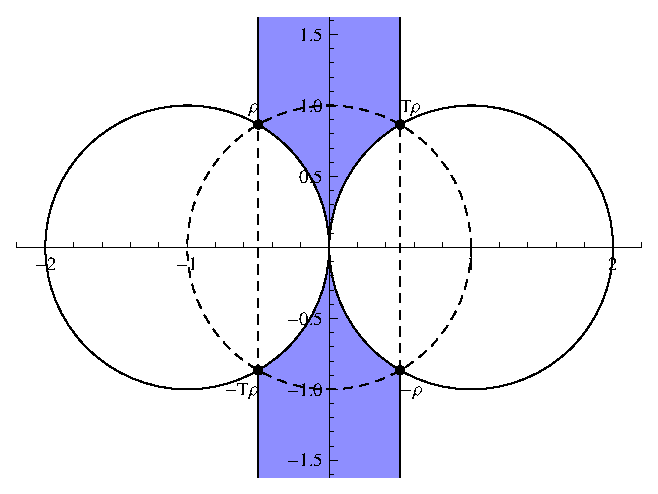
\includegraphics[width=0.7\textwidth]{figures/minimal-region}
\caption[The region $\mathcal{R} \subseteq \EC$]{The region $\mathcal{R}$ of numbers $z \in \C$ with $\abs{z + \conj{z}} < \min\{\abs{z}^2, 1\}$. It is obtained by taking the strip $\setdefsz{\big}{z \in \C}{\abs{\Re{z}} < \reci{2}}$  and cutting out two closed disks of unit radius centered about the real points $\pm 1$. The arising vertices are labeled. As usual, $T$ is the transformation $z \mapsto -\reci{z}$ and $\rho = \exp(2 \pi \ii / 3)$ is a third root of unity.}
\label{fig_PSL2MinRegion}
\end{figure}
It follows that $\mathcal{R}$ contains a fundamental region for the action of $\PSL{\Z}$ on $\EC \setminus \Irrat$. As in the homogeneous case, we see from Theorem~\ref{thm_SL2FunDomGlobMin} that equivalence of points within $\mathcal{R}$ can be established only by powers of the transformation $T \in \PSL{\Z}$. Since $T^2 = 1$, in order to obtain a fundamental region we now need to choose for each $z \in \mathcal{R}$ just exactly one of the equivalent points $z$ and $Tz$. This can for example be done such that $\abs{z} > 1$.

\index{Extended upper half-plane}
Note that for understanding the group action of $\PSL{\Z}$ on $\EC \setminus \Irrat$ it is sufficient to look at either the upper or lower half-plane of $\C$, since the group action on one half-plane is symmetric to the group action on the other half-plane by $A\conj{z} = \conj{Az}$. Let us therefore denote by $\mathcal{H}$ the upper half-plane and by $\EU$ the \emph{extended upper half-plane}:
\begin{eqnarray}
\label{eqn_Upperhalfplane}\mathcal{H} &:=& \setdefsz{\big}{z \in \C}{\Im{z} > 0} \\
\label{eqn_ExtUpperhalfplane}
\EU &:=& \mathcal{H} \cup \Q \cup \{\infty\}.
\end{eqnarray}
Clearly $\EU$ is invariant under $\PSL{\Z}$, \ie $\PSL{\Z} \EU = \EU$ and we can also consider $\PSL{\Z}$ acting on $\EU$.

\begin{theorem}
\label{thm_PSL2FunDom}
Let $\mathcal{H}$ and $\EU$ be defined as above. The set
\begin{equation}
\tilde{\FunDom} := \setdefsz{\bigg}{z \in \C}{\abs{\Re{z}} < \reci{2} \text{ and } \abs{z} > 1}
\end{equation}
is a fundamental region for the action of $\PSL{\Z}$ on $\EC \setminus \Irrat$. The part of $\tilde{\FunDom}$ lying in the upper half-plane $\mathcal{H}$, \ie the set
\begin{equation}
\label{eqn_PSL2FunDom}
\FunDom := \tilde{\FunDom} \cap \mathcal{H}
\end{equation}
is a fundamental region for the action of $\PSL{\Z}$ on $\EU$.
\end{theorem}
\begin{proof}
The second statement that $\FunDom = \tilde{\FunDom} \cap \mathcal{H}$ is fundamental region for $\PSL{\Z}$ acting on $\EU$ is a simple consequence of the first statement. For proving that $\tilde{\FunDom}$ is fundamental,  observe that $\tilde{\FunDom}$ is exactly the set
\begin{equation*}
\tilde{\FunDom} = \mathcal{R} \cap \setdefsz{\Big}{z \in \C}{\abs{z} > 1},
\end{equation*}
with $\mathcal{R}$ defined as in (\ref{eqn_PSL2MinRegion}) -- compare also Figure~\ref{fig_PSL2MinRegion}. Obviously $\tilde{\FunDom}$ is a nonempty open subset of $\mathcal{R}$, which is why two distinct points of $\tilde{\FunDom}$ can be equivalent only by the transformation $T$. However, since $\abs{z} > 1$ implies $\abs{Tz} = \abs{-1/z} < 1$, this is impossible. Therefore $\tilde{\FunDom}$ contains no equivalent distinct points.

It remains to show that every $z = \frac{u}{v} \in \mathcal{S}$ is equivalent to a point of the topological closure $\topcl{\tilde{\FunDom}}$ of $\tilde{\FunDom}$. For this purpose apply the algorithm of Theorem~\ref{thm_SL2FunDomAlg} to the vector $({}^u_v) \in \hat{\mathcal{S}}$ in order to obtain a transformation $B \in \PSL{\Z}$ which maps $z$ to a point of $\topcl{\mathcal{R}}$. It then follows that at least one of the points $Bz$ or $TBz$ lies in $\topcl{\tilde{\FunDom}}$.
\end{proof}

We now wish to obtain a \emph{fundamental set} for the action of $\PSL{\Z}$ on $\EU$. For this purpose we need to consider the boundary of $\FunDom$ and to investigate equivalent boundary points and their associated transformations. It turns out that we can define a fundamental set for the action of $\PSL{Z}$ on $\EU$ the following way:

\begin{theorem}[The fundamental set $\FunSet$]
\label{thm_PSL2FunSet}
Denote by $\FunDom$ the fundamental region from (\ref{eqn_PSL2FunDom}). The boundary of $\FunDom$ shall be segmented into the four ``boundary arcs'',
\begin{eqnarray*}
a &:=& \setdefsz{\bigg}{-\reci{2} + y \ii}{y \ge \frac{\sqrt{3}}{2}} \cup \{\infty\},\\
b &:=& \setdefsz{\bigg}{+\reci{2} + y \ii}{y \ge \frac{\sqrt{3}}{2}} \cup \{\infty\},\\
c &:=& \setdefsz{\Big}{\ii \cdot \epo{+\ii \phi}}{0 \le \phi \le \frac{\pi}{6}},\\
d &:=& \setdefsz{\Big}{\ii \cdot \epo{-\ii \phi}}{0 \le \phi \le \frac{\pi}{6}}.
\end{eqnarray*}
These boundary arcs are mapped onto each other by $Ua = b$ and $Tc = d$. The set
\begin{equation}
\label{eqn_PSL2FunSet}
\FunSet := \FunDom \cup a \cup c
\end{equation}
is a fundamental set for the action of $\PSL{\Z}$ on the extended upper half-plane $\EU$.
\end{theorem}
\begin{proof}
It follows from Theorem~\ref{thm_SL2FunDomGlobMin} that equivalence of boundary points of $\FunDom$ can only be established by transformations $A \in \PSL{Z}$ with $n(A) \le 3$. The full list of candidate transformations therefore comprises of 9 transformations: $T$, $U$, $TU$, $UT$, $TUT$ and the respective inverse transformations (note that $T$ is self-inverse). After looking at these transformations individually, it turns out that in fact only $T$ and $U$ (and $\inv{U}$) map boundary points to boundary points. Indeed $Ua = b$ and $Tc = d$ can readily be seen.
\end{proof}

\begin{remark}
\label{rem_PSL2FunDomGenDisks}
\begin{figure}
\centering
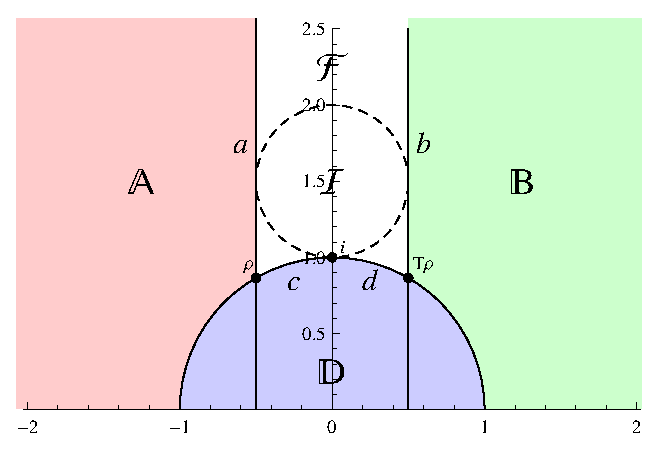
\includegraphics[width=0.8\textwidth]{figures/fundom}
\caption[The fundamental region $\FunDom$ for the action of $\PSL{\Z}$ on $\EU$]{The fundamental region $\FunDom$ for the action of the modular group $\PSL{\Z}$ on the extended upper half-plane $\EU$. It is bounded by ``generalized arcs'' $a$, $b$, $c$ and $d$ which correspond to the generalized disks $\mathbb{A}$, $\mathbb{B}$ and the unit disk $\mathbb{D}$. There is a unique disk $\Indisk \subseteq \FunDom$ which is tangent to $\mathbb{A}$, $\mathbb{B}$ and $\mathbb{D}$.}
\label{fig_PSL2FunDom}
\end{figure}
In Figure~\ref{fig_PSL2FunDom}, we see that the fundamental region $\FunDom$ can also be described in terms of generalized disks (see Definition~\ref{dfn_GenDisk}): With the terminology of Theorem~\ref{thm_PSL2FunSet}, the boundary arcs $a$ and $b$ are indeed ``generalized arcs'' of the closed generalized disks $\mathbb{A}$ and $\mathbb{B}$. Their defining matrices are
\begin{equation*}
\mathbb{A} : \mat{0}{1}{1}{1} \quad \text{and} \quad 
\mathbb{B} : \mat{\phantom{+}0}{-1}{-1}{\phantom{+}1}.
\end{equation*}
The boundary arcs $c$ and $d$ are part of the boundary of the closed unit disk $\mathbb{D}$, given by the matrix
\begin{equation*}
\mathbb{D} : \mat{1}{\phantom{+}0}{0}{-1}.
\end{equation*}
We see that the fundamental region $\FunDom$ can be characterized as set complement of the union of these three closed g-disks:
\begin{equation}
\label{eqn_PSL2FunDomDiskComplement}
\FunDom = \EU \setminus \left(\mathbb{A} \cup \mathbb{B} \cup \mathbb{D}\right).
\end{equation}
\end{remark}

\begin{definition}
\label{dfn_PSL2Indisk}
\index{Indisk}
Let the generalized disks $\mathbb{A}$, $\mathbb{B}$ and $\mathbb{D}$ be defined as in Remark~\ref{rem_PSL2FunDomGenDisks}. The unique (open) g-disk $\Indisk \subseteq \FunDom$, which is tangent to $\mathbb{A}$, $\mathbb{B}$ and $\mathbb{D}$ is called the \emph{indisk} $\Indisk$ of the fundamental region $\FunDom$. Its defining matrix is given by
\begin{equation}
\label{eqn_PSL2Indisk}
\Indisk : \mat{2}{-3\ii}{3\ii}{4}.
\end{equation}
\end{definition}



% ----------------------------------------------------- Section: Modular tiling
\section{The modular tessellation of the upper halfplane}

Since $\FunSet$ is a fundamental set for the action of $\PSL{\Z}$ on $\EU$, its images under all modular transformations cover the extended upper halfplane $\EU$ -- compare also Remark~\ref{rem_FunSetUniqueElement}. Thus for a point $z \in \EU$ there exists a transformation $A \in \PSL{\Z}$ such that $z \in A\FunSet$. We can effectively determine such a transformation by adopting the algorithm of Theorem~\ref{thm_SL2FunDomAlg}:

\begin{theorem}[The fundamental set algorithm]
Let $z \in \EU$ be a point of the extended upper halfplane and let the fundamental set $\FunSet$ be defined as in (\ref{eqn_PSL2FunSet}). A transformation $A$ satisfying $z \in A \FunSet$ can be found by performing the following steps:
\begin{enumerate}
\item Set $j := -1$ and $B_0 := 1$.
\item \label{itm_PSL2FunSetAlgLoop}
Increment $j$ by one and set $z_j := B_j z$. If $z_j \in \FunSet$, then goto step \ref{itm_PSL2FunSetAlgDone}.
\item \label{itm_PSL2FunSetAlgEjDef}
Set $e_j := \floor{\Re{z_j} + \reci{2}}$. 
\item \label{itm_PSL2FunSetAlgNext}
If $z_j - e_j \in \FunSet$, set $B_{j+1} := U^{-e_j}B_j$ -- else set $B_{j+1} := TU^{-e_j}B_j$.
\item Continue with step \ref{itm_PSL2FunSetAlgLoop}.
\item \label{itm_PSL2FunSetAlgDone} 
The desired matrix $A$ is given by $A = \inv{B_j}$.
\end{enumerate}
\end{theorem}
\begin{proof}
Note that the above is essentially a reformulation of the algorithm of Theorem~\ref{thm_SL2FunDomAlg} with the following modifications:
\begin{enumerate}[\quad (a)]
\item The algorithm is reformulated for the inhomogeneous case. The numbers $z_j$ from above and the vectors $x_j$ from the proof of Theorem~\ref{thm_SL2FunDomAlg} correspond by $z_j = \pi(x_j)$.
\item \label{itm_PSL2FunDomAlgModNint}
Instead of using the $\nint{}$ function, we use the above definition  for determining the coefficients $e_j$ -- see step \ref{itm_PSL2FunSetAlgEjDef}. This is to ensure that $z_j - e_j \in [-\reci{2}, \reci{2})$ -- otherwise we would have problems with the termination of the algorithm for the case when some $z_j$ lies on the boundary arc $b$ (as defined in Theorem~\ref{thm_PSL2FunSet}).
\item Theorem~\ref{thm_SL2FunDomAlg} yields a final vector $x_n$ such that $w := \pi(x_n) \in \topcl{\mathcal{R}}$, where $\mathcal{R}$ is defined as in (\ref{eqn_PSL2MinRegion}). In order to obtain a point in $\FunSet \subseteq \topcl{\mathcal{R}}$, we need to apply to $w$ possibly $T$ and -- if this point lies on the boundary arc $b$ -- possibly $U^{-1}$. We take this into account by explicitly checking whether the application of $T$ in the last iteration of the algorithm is necessary or not (see step \ref{itm_PSL2FunSetAlgNext}) and by the modification discussed in (\ref{itm_PSL2FunDomAlgModNint}).\qedhere
\end{enumerate}
\end{proof}

\begin{figure}
\centering
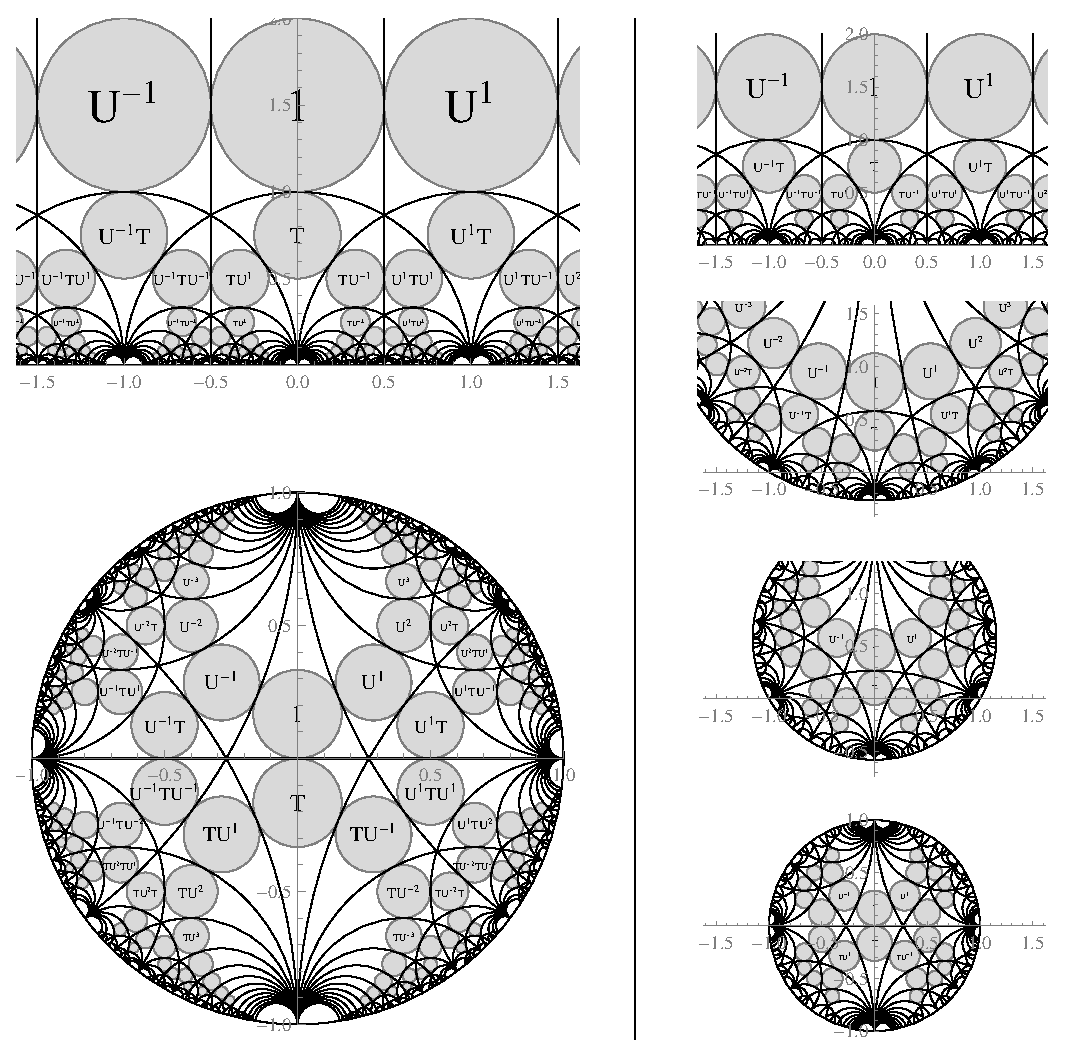
\includegraphics[width=\textwidth]{figures/modular-tiling-1}
\caption{The modular tessellation. The images of $\FunDom$ and $\Indisk$ under all modular transformations (top left) are mapped to the unit circle by the modified Cayley transform $\ModCayley$ (bottom left). A continuous transition between these two images is induced by a quarter-turn of the Riemann sphere and can be seen on the right.}
\label{fig_ModularTiling}
\end{figure}
\index{Tessellation}
\index{Modular!tessellation}
In Figure~\ref{fig_ModularTiling} on the top-left, we see the images of the fundamental region $\FunDom$ and its indisk $\Indisk$ under the transformations of the modular group. Each of these images $A \FunDom$ \resp $A \Indisk$ is labeled by the $T$-$U$ word representation of the corresponding transformation $A \in \PSL{\Z}$. We call this covering of $\EU$ by images of $\FunDom$ the \emph{modular tessellation} of the upper halfplane.

For visualization purposes, the upper halfplane has the obvious disadvantage that we can never see the whole picture. Moreover the true symmetry of the modular tessellation with respect to the transformation $T$ cannot be seen either, but it can be revealed by taking on a different view on the upper halfplane: We have seen in Example~\ref{ex_ModCayleyTransform} that the modified cayley transform $\ModCayley$ maps the upper halfplane to the unit disk. We can therefore use $\ModCayley$ to translate the modular tessellation to the unit disk. This means instead of looking at the regions $A \FunDom$ \resp $A \Indisk$ for all $A \in \SL{\Z}$, we can alternatively depict the regions $\ModCayley A \FunDom$ and the corresponding incircles $\ModCayley A \Indisk$ which is done in the bottom-left picture of Figure~\ref{fig_ModularTiling}. 

For a better understanding of this transformed representation of the modular tessellation, let us identify the drawing area with $\R^2$ rather than with $\C$. Now we note that the point $(0,1)$ corresponds to the point $\infty \in \EU$, the points $(\pm 1, 0)$ relate to $\pm 1 \in \EU$ respectively and the point $(0,-1)$ refers to $0 \in \EU$. The center $(0,0)$ represents the imaginary unit $\ii \in \EU$. In other words, as can be seen in the right column of Figure~\ref{fig_ModularTiling}, $\ModCayley$ bends the real axis to a circle\footnote{In fact, the real axis plus the point $\infty$ can be considered as generalized circle already.}, gluing together its ends at the point $\infty$ and enclosing the upper halfplane in its interior. As we have seen in Example~\ref{ex_ModCayleyTransform}, this continuous transition between the tessellation on the upper halfplane and its image under $\ModCayley$ can be explained by a quarter-turn of the Riemann sphere, compare also Figure~\ref{fig_StereoProjModCayley}.

\begin{remark}
In a more formal context, the bottom-left picture of Figure~\ref{fig_ModularTiling} can also be interpreted in two alternative ways: Firstly, we could consider a different action of $\PSL{\Z}$ on $\EC$, which we may denote as $A \ast z$ for $A \in \PSL{\Z}$ and $z \in \EC$. For its definition we make use of the natural action of the M�bius transformation $\ModCayley A \inv{\ModCayley}$:
\begin{equation*}
A \ast z := (\ModCayley A \inv{\ModCayley}) z.
\end{equation*}
Secondly, we could consider $\EC$ under the natural action of a group $G$ of M�bius transformations which is conjugate to $\PSL{\Z}$ and whose transformations are represented by matrices of a certain form over the ring of Gaussian integers $\Z[\ii]$ having determinant 1:
\begin{equation*}
G := \ModCayley \PSL{\Z} \inv{\ModCayley} = \setdefsz{\bigg}{A \in \PSL{\Z[\ii]}}{A = \mat{\alpha}{\beta}{\conj{\beta}}{\conj{\alpha}}_\sim}.
\end{equation*}
Clearly both, the action $\ast$ of $\PSL{\Z}$ as well as the natural action of $G$, leave the unit disk $\ModCayley \mathcal{H}$ invariant. Consequently $\ModCayley \FunDom$ is a fundamental region for both (equivalent) actions on the unit disk. Now the bottom-left picture of Figure~\ref{fig_ModularTiling} can be interpreted as the tessellation induced by either of these two actions with respect to the fundamental region $\ModCayley \FunDom$.
\end{remark}


% ------------------------------------------------ Section: Hyperbolic Geometry
\section{Hyperbolic geometry}

It is the goal of this section to introduce a general method for the construction of fundamental regions with respect to the action of $\PSL{\Z}$ and its subgroups on $\EU$ which relies on the concepts of 2-dimensional hyperbolic geometry. Brief introductions to the topic of hyperbolic geometry may also be found in \Lehner{}, p.\ 78ff.\footnote{Chapter II, section 12}\ and \Mumford{}, p.\ 377ff.

\index{Hyperbolic!geometry}
Plane (\ie 2-dimensional) hyperbolic geometry is obtained from 2-di\-men\-si\-o\-nal Euclidean geometry by replacing the parallel postulate by the following axiom: 
\begin{enumerate}[(A)]
\item
\emph{Let $X$ be a point and $L$ be a line on the (hyperbolic) plane, such that $L$ does not pass through $X$. Then there is more than one line $L^\prime$ passing through $X$ which does not meet $L$.}
\end{enumerate}

There are various mathematical models of hyperbolic geometry. We will use a model based on the notions of generalized disks and generalized circles which we introduced in Section~\ref{sec_GenCircles}.

\begin{definition}[Elements of hyperbolic geometry]
\label{def_HypGeomModel}
\index{Proper point}
\index{Improper point}
\index{Hyperbolic!line}
\index{Hyperbolic!plane}
\index{H-line}
\index{H-plane}
\index{Horizon}
Let $\mathcal{P} \subseteq \C$ be a generalized disk, which serves as a model for 2-dimensional hyperbolic geometry. In this context, we will refer to $\mathcal{P}$ as \emph{hyperbolic plane} (for short \emph{h-plane}). The interior points of $\mathcal{P}$ are called \emph{proper points}; the boundary points of $\mathcal{P}$ are called \emph{improper points}. The set of all improper points (which is a generalized circle) is called the \emph{horizon} of $\mathcal{P}$.\footnote{The notions of proper and improper points as well as horizon are taken over from \Fenchel{}.} Every generalized circle $C$, which intersects the horizon of $\mathcal{P}$ orthogonally in two distinct (improper) points, gives rise to exactly one \emph{hyperbolic line} (for short \emph{h-line}) $L$ which is given by $L = C \cap \mathcal{P}$. 
\end{definition}

In the above model of hyperbolic geometry, the angular measure is taken over from Euclidean geometry, \ie the angle enclosed by two h-lines which intersect each other in a proper point $z \in \mathcal{P}$ is defined as the Euclidean angle enclosed by the (Euclidean) tangents of the h-lines at the point $z$. It now remains to introduce a measure for the distance between proper points in $\mathcal{P}$.

\begin{definition}[Metric]
\index{Metric}
Let $\mathcal{S}$ be nonempty a set. A function $d : \mathcal{S} \times \mathcal{S} \to \R$ is a \emph{metric} on $\mathcal{S}$, if the following conditions are satisfied for all $x,y,z \in \mathcal{S}$:
\begin{enumerate}[(i)]
\item \label{itm_MetricNonneg}
\emph{Non-negativity:} $d(x,y) \ge 0$.
\item \label{itm_MetricCoincidence}
\emph{Coincidence axiom:} $d(x,y) = 0$ if and only if $x = y$.
\item \label{itm_MetricSymmetry}
\emph{Symmetry:} $d(x,y) = d(y,x)$.
\item \label{itm_MetricTriIneq}
\emph{Triangle inequality:} $d(x,z) \le d(x,y) + d(y,z)$.
\end{enumerate}
\end{definition}
\begin{remark} From
\begin{equation*}
0 = d(x,x) \le d(x,y) + d(y,x) = 2 d(x,y),
\end{equation*}
we see that non-negativity (\ref{itm_MetricNonneg}) is implied by the conditions (\ref{itm_MetricCoincidence}), (\ref{itm_MetricSymmetry}) and (\ref{itm_MetricTriIneq}).
\end{remark}

\begin{definition}[Isometry]
\label{dfn_IsometryRigidMotion}
\index{Isometry}
Let $\mathcal{S}$ be a set and $d$ be a metric on $\mathcal{S}$. A map $\phi : \mathcal{S} \to \mathcal{S}$ is called an \emph{isometry}, if it leaves distances invariant, \ie if
\begin{equation*}
d(x,y) = d(\phi(x), \phi(y)) \quad \text{for all } x,y \in \mathcal{S}.
\end{equation*}
\end{definition}

\begin{remark}
It is direct to see that the set of all bijective isometries forms a group under the operation of function composition. Note that the coincidence axiom (\ref{itm_MetricCoincidence}) implies that isometries are necessarily injective. However, in general they do not need to be surjective.
\end{remark}

\index{Rigid motion}
We wish to introduce a metric on the h-plane $\mathcal{P}$, such that every M�bius transformation which maps $\mathcal{P}$ onto itself is an isometry of $\mathcal{P}$. Clearly all M�bius transformations with this property form a group. We will refer to the transformations of this group as \emph{rigid motions}\footnote{A rigid motion is an isometry which additionally leaves angles and their orientation invariant.} of the h-plane. 

\index{Cross ratio}
For the definition of such a metric we will take advantage of the so-called \emph{cross ratio}. Note that in literature for the term ``cross ratio'' different notations and definitions are used. We will in this regard adhere to \Caratheodory{}, whose derivation of the cross ratio's elementary properties is particularly concise and elegant.

\begin{definition}
\label{dfn_CrossRatio}
Let $z_1,z_2,z_3,z_4 \in \EC$ be numbers of the extended complex plane with the restriction that at most two of these numbers are equal. The \emph{cross-ratio} $(z_1,z_2,z_3,z_4) \in \EC$ is defined as
\begin{equation}
\label{eqn_CrossRatio}
(z_1,z_2,z_3,z_4) := \crossrat{z_1}{z_2}{z_3}{z_4}.
\end{equation}
Note that in the case of an infinite quantity $z_k = \infty$, the cross ratio  shall be evaluated by formally dividing the two respective factors in the numerator and denominator of (\ref{eqn_CrossRatio}) by $z_k$ and by substitution of expressions $\reci{\infty}$ with zero.
\end{definition}

We will need the following important properties of the cross ratio:

\begin{lemma}[Invariance under M�bius transformations]
\label{lem_CrossRatioInvariance}
Let $\phi \in \PGL{\C}$ be a M�bius transformation and $z_1,z_2,z_3,z_4 \in \EC$ such that their cross ratio is defined. Set $w_j := \phi(z_j)$ for $j \in \{1,2,3,4\}$. The cross ratios of the numbers $z_j$ and $w_j$ are equal, \ie
\begin{equation}
\label{eqn_CrossRatioInvariance}
(z_1,z_2,z_3,z_4) = (w_1,w_2,w_3,w_4).
\end{equation}
\end{lemma}
\begin{proof}[Sketch of proof]
Let us write the M�bius transformation $\phi$ as $\phi(z) = \moebius{a}{b}{c}{d}{z}$. For $i,j \in \{1,2,3,4\}$, we have
\begin{equation*}
w_i - w_j 
= \moebius{a}{b}{c}{d}{z_i} - \moebius{a}{b}{c}{d}{z_j} 
= \frac{ad - bc}{(c z_i + d)(c z_j + d)} \cdot (z_i - z_j).
\end{equation*}
Consequently, if we define
\begin{equation*}
A := \frac{(ad - bc)^2}{(c z_1 + d)(c z_2 + d)(c z_3 + d)(c z_4 + d)},
\end{equation*}
we obtain
\begin{equation*}
(w_1 - w_2)(w_3 - w_4) = A(z_1 - z_2)(z_3 - z_4).
\end{equation*}
On the other hand, exploiting the symmetry of $A$ with respect to the numbers $z_j$, we have
\begin{equation*}
(w_1 - w_3)(w_2 - w_4) = A(z_1 - z_3)(z_2 - z_4).
\end{equation*}
In the case when all involved numbers $z_j$ and $w_j$ are finite (and in particular $A$ is finite and nonzero), division of these two equations yields (\ref{eqn_CrossRatioInvariance}). The prove of the general case, when one or two of the numbers $z_j$ (\resp $w_j$) are $\infty$, involves some inconvenient case distinctions which we will not carry out here.
\end{proof}

\begin{lemma}
\label{lem_CrossRatioMoebius}
Let $z_1, z_2, z_3 \in \EC$ be pairwise distinct. The function
\begin{equation}
\label{eqn_CrossRatioMoebius}
\fundef{\lambda}{\EC}{\EC}{z}{(z_1,z_2,z_3,z)}
\end{equation}
is a M�bius transformation and satisfies $\lambda(z_1) = 1$, $\lambda(z_2) = \infty$, $\lambda(z_3) = 0$.
\end{lemma}
\begin{proof}[Sketch of proof]
In the case when $\infty \notin \{z_1,z_2,z_3\}$, by setting $a := z_2 - z_1$, $b := z_2 (z_1 - z_2)$, $c := z_3 - z_1$ and $d := z_2 (z_1 - z_3)$ we can obviously write 
\begin{equation*}
\lambda(z) = \crossrat{z_1}{z_2}{z_3}{z} = \moebius{a}{b}{c}{d}{z}.
\end{equation*}
Moreover, we have
\begin{equation*}
ad - bc = (z_1 - z_2)(z_2 - z_3)(z_3 - z_1).
\end{equation*}
By assumption the numbers $z_j$ are pairwise distinct and therefore $\lambda$ is indeed a M�bius transformation. Note that for the other case, when some $z_k = \infty$, the cross ratio needs to be evaluated as specified in Definition~\ref{dfn_CrossRatio} and the coefficients $a,b,c,d$ need to be adapted appropriately. The statement on the images of $z_1,z_2,z_3$ under $\lambda$ is readily verified.
\end{proof}

\begin{corollary}
\label{cor_CrossRatioGCircle}
Denoting the extended real axis by $\R_\infty := \R \cup \{\infty\}$, the map $\lambda : \EC \to \EC$ from (\ref{eqn_CrossRatioMoebius}) satisfies $\lambda(z) \in \R_\infty$ if and only if $z$ lies on the generalized circle which is determined by the points $z_1,z_2,z_3$.
\end{corollary}
\begin{proof}
This statement is a consequence of the fact that $\lambda$ is a M�bius transformation and therefore maps the g-circle determined by the points $z_1,z_2,z_3$ pointwise one-to-one to the extended real axis $\R_\infty$.
\end{proof}

The above properties of the cross ratio allow to define a metric on the hyperbolic plane $\mathcal{P}$ the following way:

\begin{definition}[\Poincare{} metric]
\label{dfn_PoincareMetric}
\index{Poincar{\'e}!metric}
\index{Hyperbolic!distance}
Let $z_1, z_2 \in \mathcal{P}$ be two distinct proper points of the hyperbolic plane and let $L$ be the unique h-line joining $z_1$ with $z_2$. Label the two (improper) endpoints of $L$ by $\infty_1$ and $\infty_2$, such that $\infty_1, z_1, z_2, \infty_2$ are in order along the h-line $L$. The hyperbolic distance between $z_1$ and $z_2$ is defined as
\begin{equation}
\label{eqn_PoincareMetric}
\hypdist{z_1}{z_2} := \reci{2} \log \chi \quad \text{with } \chi := (z_1,\infty_2,\infty_1,z_2).
\end{equation}
Additionally we define $\hypdist{z}{z} = 0$ for all proper points $z \in \mathcal{P}$.
\end{definition}

\begin{theorem}
The hyperbolic distance defined in $(\ref{eqn_PoincareMetric})$ is a metric on the hyperbolic plane $\mathcal{P}$ which we call the \emph{\Poincare{} metric} on $\mathcal{P}$.
\end{theorem}
\begin{proof}[Sketch of proof]
The cross ratio $\chi$ in (\ref{eqn_PoincareMetric}) may alternatively be written as $\chi = \lambda(z_2)$, where $\lambda(z) := (z_1,\infty_2,\infty_1,z)$ is, according to Lemma~\ref{lem_CrossRatioMoebius}, a M�bius transformation satisfying $\lambda(z_1) = 1$ and $\lambda(\infty_2) = \infty$. Corollary~\ref{cor_CrossRatioGCircle} ensures that $\lambda(z)$ is real for all $z$ lying on the h-line $L$. Since $\lambda$ is a continuous map, it follows that $\lambda$ maps the h-line segment $S \subseteq L$ which is bounded by the points $z_1$ and $\infty_2$ pointwise one-to-one to the interval $[1,\infty] \subseteq \R_\infty$. For this reason, the hyperbolic metric is non-negative and $\hypdist{z_1}{z_2} \to 0$ as $z_2$ approaches $z_1$ along $S$. Similarly, $\hypdist{z_1}{z_2} \to \infty$ as $z_2$ approaches $\infty_2$ along $S$.

The symmetry of $d_\text{hyp}$ can easily be verified: Note that exchanging $z_1$ and $z_2$ also swaps the roles of the improper points $\infty_1$ and $\infty_2$. We therefore need to show that $\chi_1 := (z_1,\infty_2,\infty_1,z_2) = (z_2,\infty_1,\infty_2,z_1) =: \chi_2$ which is indeed the case:
\begin{equation*}
\chi_1 = \crossrat{z_1}{\infty_2}{\infty_1}{z_2} = \crossrat{z_2}{\infty_1}{\infty_2}{z_1} = \chi_2.
\end{equation*}

By the above observations, we have $\hypdist{z_1}{z_2} = 0$ if and only if $z_1 = z_2$. Consequently the coincidence axiom is satisfied. The proof of the fact that $d_\text{hyp}$ also satisfies the triangle inequality is out of scope of this work.
\end{proof}

\begin{remark}
The hyperbolic distance along a h-line is additive, \ie for three points $z_1,z_2,z_3$ which are in order along a h-line, we have
\begin{equation*}
\hypdist{z_1}{z_3} = \hypdist{z_1}{z_2} + \hypdist{z_2}{z_3},
\end{equation*}
which is a consequence of
\begin{equation*}
\crossrat{z_1}{\infty_2}{\infty_1}{z_2} \cdot \crossrat{z_2}{\infty_2}{\infty_1}{z_3} = 
\crossrat{z_1}{\infty_2}{\infty_1}{z_3}
\end{equation*}
\end{remark}

\begin{remark}[\Poincare{} disk and half-plane model]
\label{rem_PoincareModel}
\index{Poincar{\'e}!half-plane model}
\index{Poincar{\'e}!disk model}
If we choose the upper half-plane of $\EC$ as model for the hyperbolic plane, \ie $\mathcal{P} := \topcl{\mathcal{H}}$, we obtain the \emph{\Poincare{} half-plane model} of hyperbolic geometry. If instead the unit disk is chosen, $\mathcal{P} := \mathbb{D}$, then we talk of the \emph{\Poincare{} disk model}.

Clearly both models are equivalent in the sense that one model can be obtained from the other by applying a M�bius map which transforms the upper half-plane to the unit disk (or vice-versa). For our purposes, the \Poincare{} half-plane model will be most relevant.
\end{remark}

\subsection{Normal polygons and fundamental regions}

We can now exploit the concepts of 2-dimensional hyperbolic geometry in the search of fundamental regions for the action of $\PSL{\Z}$ and its subgroups on $\EU$. 

The idea -- taken from \Lehner{} -- may be shortly described as follows: Given a subgroup $G \le \PSL{\Z}$, we fix a point $z_0 \in \mathcal{H}$ which has a trivial stabilizer $G_{z_0} = \{1\}$. The points $z$ of the sought fundamental region $\mathcal{N}_{z_0}$ shall be characterized by the property $\hypdist{z}{z_0} \le \hypdist{Az}{z_0}$ for all $A \in G$. It turns out that such a fundamental region $\mathcal{N}_{z_0}$ can be obtained by a simple geometric construction for which we will need the following notions:

\begin{definition}[Hyperbolic half-plane]
\label{dfn_HyperbolicHalfplane}
\index{Hyperbolic!half-plane}
Let $D$ be a generalized disk, such that its boundary intersects the horizon of $\mathcal{P}$ orthogonally in two distinct (improper) points. The (nonempty) set $H := D \cap \mathcal{P}$ is called a \emph{hyperbolic half-plane}.
\end{definition}

\begin{definition}[Perpendicular bisector]
\label{dfn_PerpendicularBisector}
\index{Perpendicular bisector}
Let $z_1, z_2 \in \mathcal{P}$ be two distinct proper points and denote by $S$ the unique h-line segment whose endpoints are $z_1$ and $z_2$. The set of proper points $w$ for which $\hypdist{w}{z_1} = \hypdist{w}{z_2}$ defines a h-line and is called the \emph{perpendicular bisector} of $S$. Additionally we define $H_{z_1}(z_2)$ as the hyperbolic half-plane consisting of all points $w \in \mathcal{P}$ which are closer to $z_1$ than to $z_2$:
\begin{equation}
\label{eqn_NormPolyHalfplane}
H_{z_1}(z_2) := \setdef{w \in \mathcal{P}}{\hypdist{w}{z_1} < \hypdist{w}{z_2}}.
\end{equation}
Note that the hyperbolic boundary of $H_{z_1}(z_2)$ is precisely the perpendicular bisector of the h-line segment $S$.
\end{definition}

\begin{definition}[Normal polygon]
\label{dfn_NormalPolygon}
\index{Normal polygon}
Let $G \le \PSL{\Z}$ be a subgroup of the modular group. Let $z \in \EU$ with trivial stabilizer $G_z = \{1\}$. The set
\begin{equation}
\label{eqn_NormalPolygon}
\mathcal{N}_z := \bigcap_{A \in G \setminus\{1\}} H_{z}(Az)
\end{equation}
is called the \emph{normal polygon} with respect to the group $G$ and the point $z$.
\end{definition}

\begin{remark}
The term ``normal polygon'' is justified by the fact that $\mathcal{N}_z$, as intersection of hyperbolic half-planes, is bounded entirely by h-line segments and therefore can be considered as a convex (possibly generalized) polygon\footnote{A region bounded by infinitely many h-line segments is called a generalized polygon.} in the hyperbolic sense.
\end{remark}

\begin{theorem}
Let $\mathcal{N}_z$ be a normal polygon for the group $G \le \PSL{\Z}$ with respect to the point $z \in \mathcal{H}$. $\mathcal{N}_z$ is a fundamental region for the action of $G$ on $\EU$.
\end{theorem}
\begin{proof}
For the proof of this fact in the more general context of \emph{principal circle groups}, \ie discontinuous groups of M�bius transformations fixing a given generalized circle, we refer to \Lehner{}, p.146ff.\footnote{Chapter IV, Section 7}
\end{proof}

\begin{figure}
\centering
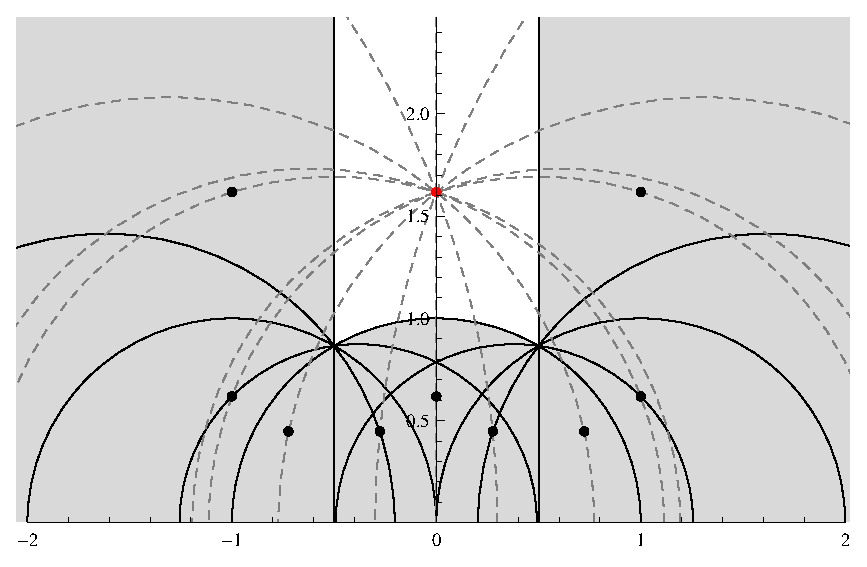
\includegraphics[width=.9\textwidth]{figures/normpoly-fundom-1}
\caption[The fundamental region $\FunDom$ as normal polygon]{The fundamental region $\FunDom$ can alternatively obtained by constructing the normal polygon with respect to a point $z$ on the imaginary axis with $\Im{z} > 1$. Above the point $z = \phi \ii$ (red) has been chosen, where $\phi = \frac{\sqrt{5}+1}{2}$ denotes the golden ratio.}
\label{fig_NormalPolyFunDom}
\end{figure}
\begin{figure}
\centering
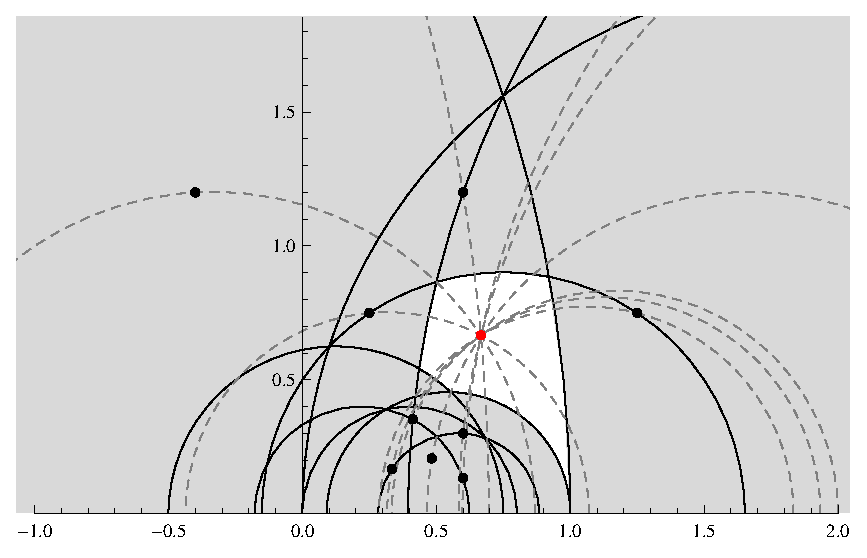
\includegraphics[width=.9\textwidth]{figures/normpoly-fundom-2}
\caption[An alternative fundamental region for $\PSL{\Z}$]{An alternative fundamental region for the action of $\PSL{\Z}$ on $\EU$. It is obtained by constructing the normal polygon for the point $\frac{2}{3}(1+\ii)$.}
\label{fig_AltNormalPolyFunDom}
\end{figure}

\begin{example}[Fundamental regions for $\PSL{\Z}$]
We see in Figure~\ref{fig_NormalPolyFunDom} that the fundamental region $\FunDom$ from (\ref{eqn_PSL2FunDom}) can alternatively be obtained by constructing the normal polygon for a point $z$ on the imaginary axis with $\Im{z} > 1$ (compare also Figure~\ref{fig_PSL2FunDom}). A different fundamental region for the action of $\PSL{\Z}$ on $\EU$ is displayed in Figure~\ref{fig_AltNormalPolyFunDom}.

In both figures, the point $z$ for which the normal polygon is constructed is colored red. Its equivalent points $Az$, $A \ne 1$ can be seen in black. For every pair $(z, Az)$, the corresponding perpendicular bisector (black) can be found best by following the gray dashed h-line which joins $Az$ with $z$.

Note that for producing an accurate picture of the normal polygon, it was in both cases sufficient to enumerate just 9 different transformations. In case of Figure~\ref{fig_NormalPolyFunDom}, all transformations with $n(A) \le 3$ have been selected, where $n(A)$ denotes the grading of $A$ as defined in (\ref{eqn_grading}). 

In Figure~\ref{fig_AltNormalPolyFunDom}, in order to achieve a good ``locality'' of the equivalent points $Az$ around $z$, additionally the fundamental set algorithm (Theorem~\ref{thm_FunSetAlg}) has been utilized: The selected transformations are all of the form $A = CB\inv{C}$ with $B \in \PSL{\Z}$, $n(B) \le 3$ and where $C$ denotes the transformation obtained when applying the fundamental set algorithm to $z$.
\end{example}

\begin{figure}
\centering
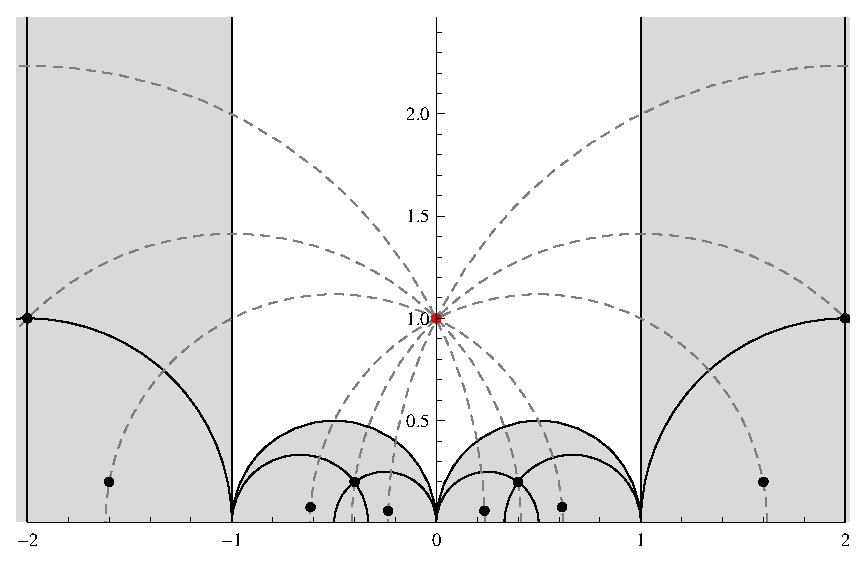
\includegraphics[width=.9\textwidth]{figures/normpoly-gamma2-1}
\caption[A fundamental region for $\Gamma(2)$]{A fundamental region for the subgroup $\Gamma(2) \le \PSL{\Z}$. It is given by the normal polygon constructed with respect to the point $\ii$.}
\label{fig_Gamma2NormalPoly}
\end{figure}

\begin{example}
\index{Principal congruence subgroup}
As a demonstration of the normal polygon method in case of a proper subgroup of $\PSL{\Z}$, we see in Figure~\ref{fig_Gamma2NormalPoly} a normal polygon for the group $\Gamma(2) \le \PSL{\Z}$. For $m \in \N$, the \emph{principal congruence subgroup} $\Gamma(m)$ is defined as
\begin{equation*}
\Gamma(m) := \setdefsz{\bigg}{\mat{a}{b}{c}{d} \in \PSL{\Z}}{a \equiv d \equiv \pm 1,\ b \equiv c \equiv 0 \mod m}.
\end{equation*}
For drawing Figure~\ref{fig_Gamma2NormalPoly}, all nontrivial transformations in $\Gamma(2)$ with a grading $\le 18$ (of which there are 12) have been selected. Note that for the particular chosen point $z$, also ``the first four'' nontrivial transformations of $\Gamma(2)$ (whose grading is $\le 6$) would have been enough for obtaining the same region.
\end{example}


% --------------------------------------- CHAPTER: ALGORITHMS AND VISUALIZATION
\chapter{Applications in visualization}

\section{The action of M�bius transformations}

So far we often talked about the action of M�bius transformations on $\EC$. However, up to now occasions have been quite rare where we literally could see them ``in action''. Maybe the most important exceptions to this are Figures~\ref{fig_StereoProjInversion} and \ref{fig_StereoProjModCayley}, showing continuous transitions between preimages and images of certain sets under the two transformations $z \mapsto \reci{z}$ and  $\ModCayley$ (the modified Cayley transform), both induced by rotations of the Riemann sphere. 

In this section we introduce a more direct method for visualization of such continuous transitions, a method working for arbitrary M�bius transformations and doing without stereographic projection and motion of Riemann spheres. For this purpose, we exploit the ``linear algebra nature'' (see Remark~\ref{rem_NatureMoebius}) of M�bius transformations. For easier notation we will not distinguish between a matrix $A \in \GL{\C}$ and the corresponding M�bius transformation ${}_\pm A \in \PGL{\C}$. In particular with $A$ will denote both, a matrix in $\GL{\C}$ and the corresponding M�bius transformation in $\PGL{\C}$.

For $A \in \GL{\C}$ and $k \in \Z$, it follows from Theorem~\ref{thm_MoebiusGroup} that matrix power $A^k$ corresponds to the M�bius transformation obtained by $k$ times composing the transformation $A$ with itself. The idea is now to generalize the concept of matrix powers from integral to real exponents. If we do so, then for any set $S \in \EC$ of interest, we can visualize the transition from $S$ to its image under $A$ simply by depicting a sequence of intermediate images $A^t S \subseteq \EC$, with a varying parameter $t \in [0,1]$.

\index{Generalized!matrix power}
In order to introduce such \emph{generalized matrix powers}, note that for integral exponents, powers of $A$ can be calculated by using its \index{Jordan normal form} \emph{Jordan normal form}.\footnote{Also called \emph{Jordan canonical form}. For more details on Jordan normal forms, Eigenvalues and Eigenvectors see for example Chapter VII, Linear algebra, in \Hungerford{}.} If $J$ is a Jordan normal form of $A$, then for some $P \in \GL{\C}$ we have $A = \inv{P} J P$ and consequently
\begin{equation}
\label{eqn_MatrixIntPower}
A^k = \inv{P} J^k P, \quad\text{for all } k \in \Z.
\end{equation}
The matrix $J$ has one of the two possible forms
\begin{equation*}
(i)\ J = \mat{\lambda_1}{0}{0}{\lambda_2} \quad\text{or}\quad 
(ii)\ J = \mat{\lambda}{1}{0}{\lambda}
\end{equation*}
and their respective matrix powers are given by
\begin{equation}
\label{eqn_JordanPower}
(i)\ J^k = \mat{\lambda_1^k}{0}{0}{\lambda_2^k} \quad\text{and}\quad
(ii)\ J^k = \mat{\lambda^k}{k \lambda^{k-1}}{0}{\lambda^k}.
\end{equation}
From here it is just a small step to the generalization of matrix powers to real exponents: We choose a fixed branch of the natural (complex) logarithm, for example such that the imaginary part of the logarithm ranges in the interval $(-\pi,\pi]$, \ie $\Im{\ln z} = \arg z \in (-\pi,\pi]$ for all $z \in \C$. Now we can evaluate $\lambda^k$, for $\lambda \in \C$ and $k \in \R$, as $\lambda^k := \exp(k \ln \lambda)$.

\begin{definition}[Generalized matrix power]
\label{dfn_GenMatPower}
Let $A \in \GL{\C}$ be a matrix. For $k \in \R$ we say $B$ is an $k$-th power of $A$, in symbols $B = A^k$, if there is a $P \in \GL{\C}$ such that
\begin{equation*}
A = \inv{P} J P \quad \text{and} \quad B = \inv{P} J^k P,
\end{equation*}
where $J$ is in Jordan normal form and $J^k$ is defined through (\ref{eqn_JordanPower}), choosing a fixed branch of the natural logarithm and evaluating the expressions $\lambda^k$ as $\lambda^k := \exp(k \ln \lambda)$.
\end{definition}

\begin{remark}[Eigenvectors and fixed points]
Writing the matrix $P$ in the form $P = (v_1 \mid v_2)$ with $v_1, v_2 \in \C^2$, in case $(i)$, $v_1$ and $v_2$ are \index{Eigenvector} \emph{eigenvectors} of $A$ corresponding to the \index{Eigenvalue} \emph{eigenvalues} $\lambda_1$ and $\lambda_2$ respectively. In case $(ii)$, only $v_1$ is an eigenvector ($v_2$ is a \index{Generalized!eigenvector} \emph{generalized eigenvector}). It is worth noting that a vector $({}^u_v) \in \C^2$ is an eigenvector of $A \in \GL{\C}$, if and only if $u/v \in \EC$ is a fixed point for the M�bius transformation $A$:
\begin{equation*}
A \cdot \cvec{u}{v} = \lambda \cvec{u}{v} \quad\Leftrightarrow\quad
A \left(\frac{u}{v}\right) = \frac{\lambda u}{\lambda v} = \frac{u}{v}.
\end{equation*}
Therefore, in case $(i)$, $A$ is either the identity transformation or has exactly two distinct fixed points. In case $(ii)$, $A$ has exactly one fixed point.
\end{remark}

As Definition~\ref{dfn_GenMatPower} already suggests, generalized matrix powers are not unique but depend on the chosen branch of the natural logarithm. The following Example will illustrate this:
\begin{example}
\label{ex_InversionSqrt}
Let $A = \smallmat{0}{1}{1}{0} \in \GL{\C}$ be the matrix corresponding to the M�bius map $z \mapsto \reci{z}$. We wish to calculate the ``square root'' $A^{\reci{2}}$ of this transformation. The eigenvalues of $A$ are $\lambda_1 = -1$ and $\lambda_2 = 1$; the corresponding eigenvectors are $v_1 = ({}^{-1}_{\phantom{+}1})$ and $v_2 = ({}^1_1)$. We can therefore write $A$ as
$A = \inv{P} J P$ with $P = \smallmat{-1}{1}{\phantom{+}1}{1}$ and $J = \smallmat{-1}{0}{\phantom{+}0}{1}$.
Next we calculate $J^{\reci{2}}$ by evaluating $\exp(\reci{2} \ln \lambda_1)$ and $\exp(\reci{2} \ln \lambda_2)$. Choosing a logarithm branch such that $\Im{\ln z} \in (-\pi,\pi]$ for all $z \in \C$, and denoting equivalence of matrices in $\PGL{\C}$ again by $\sim$, this yields $J^{\reci{2}} = \smallmat{\ii}{0}{0}{1}$ and
\begin{equation*}
A^{\reci{2}} = \inv{P}J^{\reci{2}}P = \reci{2} \mat{1+\ii}{1-\ii}{1-\ii}{1+\ii} \sim \mat{\ii}{1}{1}{\ii}.
\end{equation*}
We therefore see that $A^\reci{2} = \ModCayley$ and the modified Cayley transform is in this sense a ``square root'' of the transformation $A : z \mapsto \reci{z}$, compare also Example~{\ref{ex_ModCayleyTransform}}.

In contrast to that, choosing a slightly different logarithm branch, such that $\Im{\ln z} \in [-\pi,\pi)$ for all $z \in \C$, we get $\exp(\reci{2} \ln \lambda_2) = -\ii$ and obtain a matrix conjugate to the above one:
\begin{equation*}
A^{\reci{2}} = \reci{2} \mat{1-\ii}{1+\ii}{1+\ii}{1-\ii} \sim \mat{-\ii}{1}{1}{-\ii}.
\end{equation*}
Note that this second transformation, just like the modified Cayley transformation, can also be considered as a quarter-turn of the Riemann sphere around the $x_1$ axis, but it rotates in the opposite direction and maps the \emph{lower} halfplane to the unit disk.
\end{example}

\begin{example}
As an application of generalized matrix powers, we can visualize the action of the modular transformations $U : z \mapsto z+1$, $T: z \mapsto -\reci{z}$ and $R: z \mapsto -\reci{z+1}$ on the modular tessellation. For the parameter $t \in [0,1]$ ``intermediate actions'' of these maps are given through the M�bius maps corresponding to the matrices
\begin{eqnarray*}
U^t &\sim& \mat{1}{t}{0}{1},\\
T^t &\sim& \mat{\cos \left(\frac{\pi t}{2}\right)}{-\sin \left(\frac{\pi t}{2}\right)}{\sin \left(\frac{\pi t}{2}\right)}{\cos \left(\frac{\pi  t}{2}\right)},\\
R^t &\sim& \mat{\sqrt{3} \cos \left(\frac{\pi t}{3}\right)-\sin \left(\frac{\pi t}{3}\right)}{-2 \sin \left(\frac{\pi t}{3}\right)}{2 \sin \left(\frac{\pi t}{3}\right)}{\sqrt{3} \cos \left(\frac{\pi t}{3}\right)+\sin \left(\frac{\pi t}{3}\right)}.
\end{eqnarray*}

In Figures~\ref{fig_UAction}, \ref{fig_TAction} and \ref{fig_RAction} we can see the modular tessellation and its ``intermediate images'' under the transformations $T$, $U$ and $R$ for the parameter values $t \in \{0, \reci{5}, \frac{2}{5}, \frac{3}{5}, \frac{4}{5}, 1\}$. Again we use the modified Cayley transform to map the tessellation of the upper halfplane to the unit disk. Looking at Figure~\ref{fig_TAction}, another advantage of seeing the upper halfplane from this different angle gets apparent: Under $\ModCayley$, the action of $T$ corresponds to a simple rotation by $180^\circ$ around the fixed point $\ii$. This is in close connection with Remark~\ref{rem_TRotation}, where we noted that $T$ corresponds to a half-turn of the Riemann sphere around the $x_2$ axis. Finally we can see in Figure~\ref{fig_RAction} that, with a slight distortion, $R$ corresponds to a rotation by $120^\circ$ around the fixed point $\rho = \exp(2 \pi \ii / 3)$.

Note that the individual frames in Figures~\ref{fig_UAction}, \ref{fig_TAction} and \ref{fig_RAction} have been arranged such that the first column has to be read first in top-down direction and then the second column has to be read in bottom-up direction, allowing in the first row a direct comparison of the tessellation's preimage and image under the respective transformations.
\begin{figure}
\centering
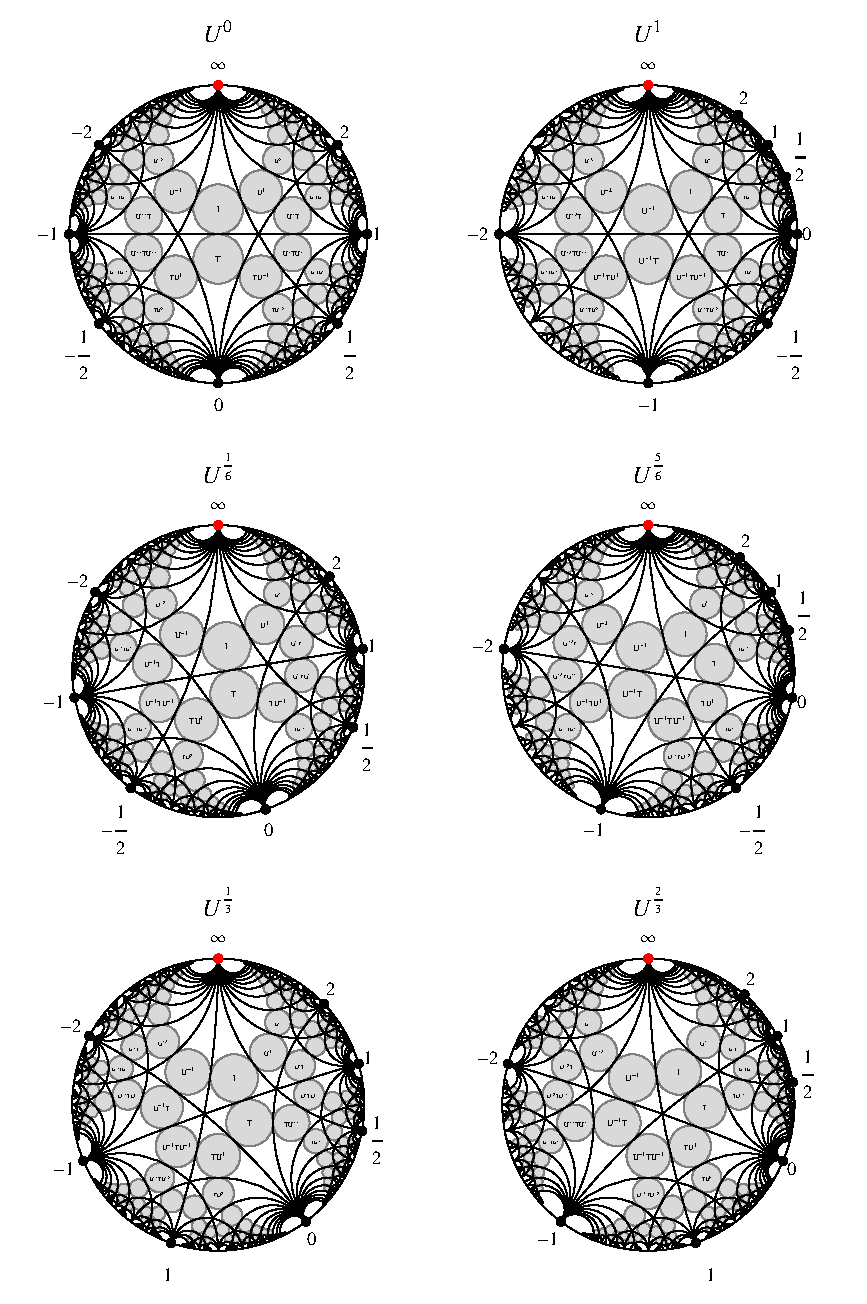
\includegraphics[width=\textwidth]{figures/u-action}
\caption{The action of $U : z \mapsto z+1$.}
\label{fig_UAction}
\end{figure}

\begin{figure}
\centering
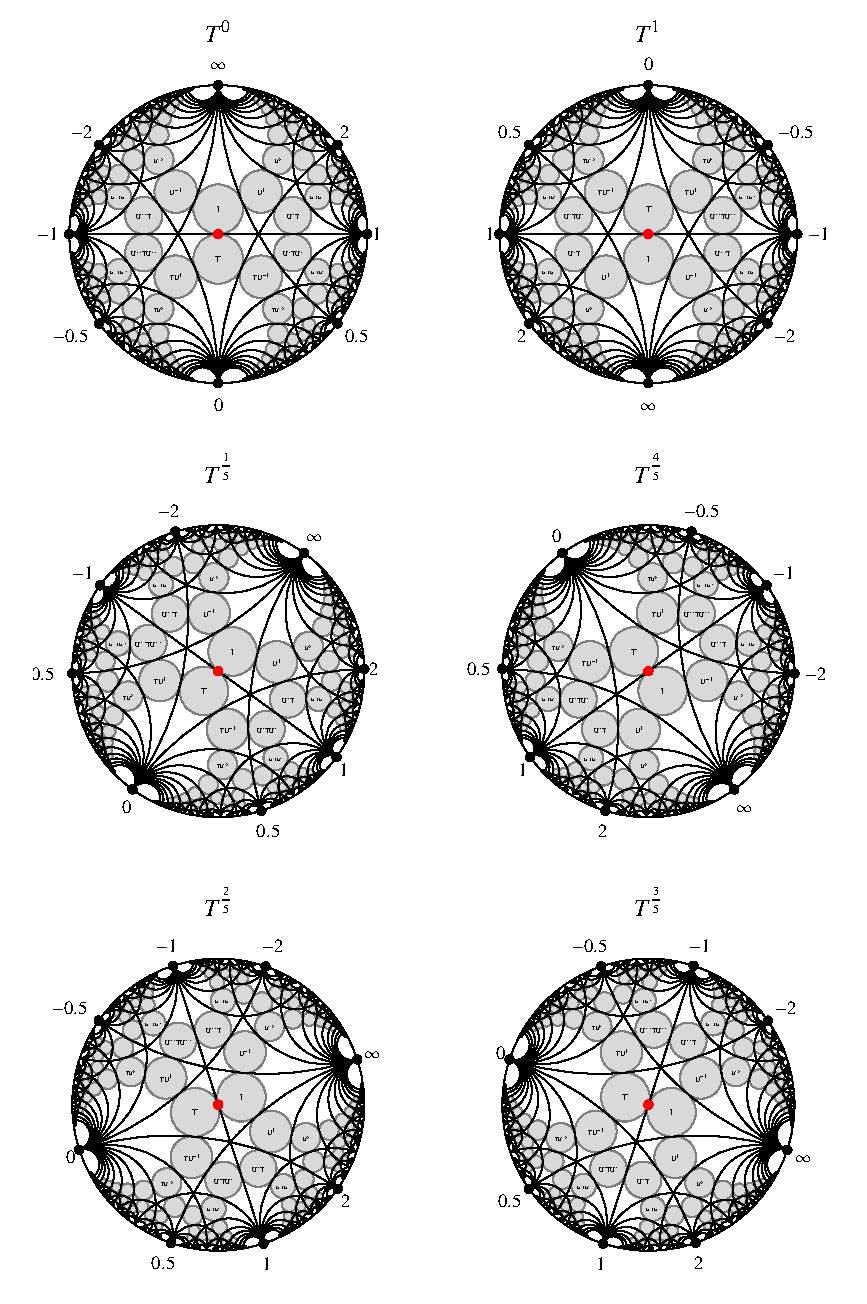
\includegraphics[width=\textwidth]{figures/t-action}
\caption{The action of $T : z \mapsto -\reci{z}$.}
\label{fig_TAction}
\end{figure}

\begin{figure}
\centering
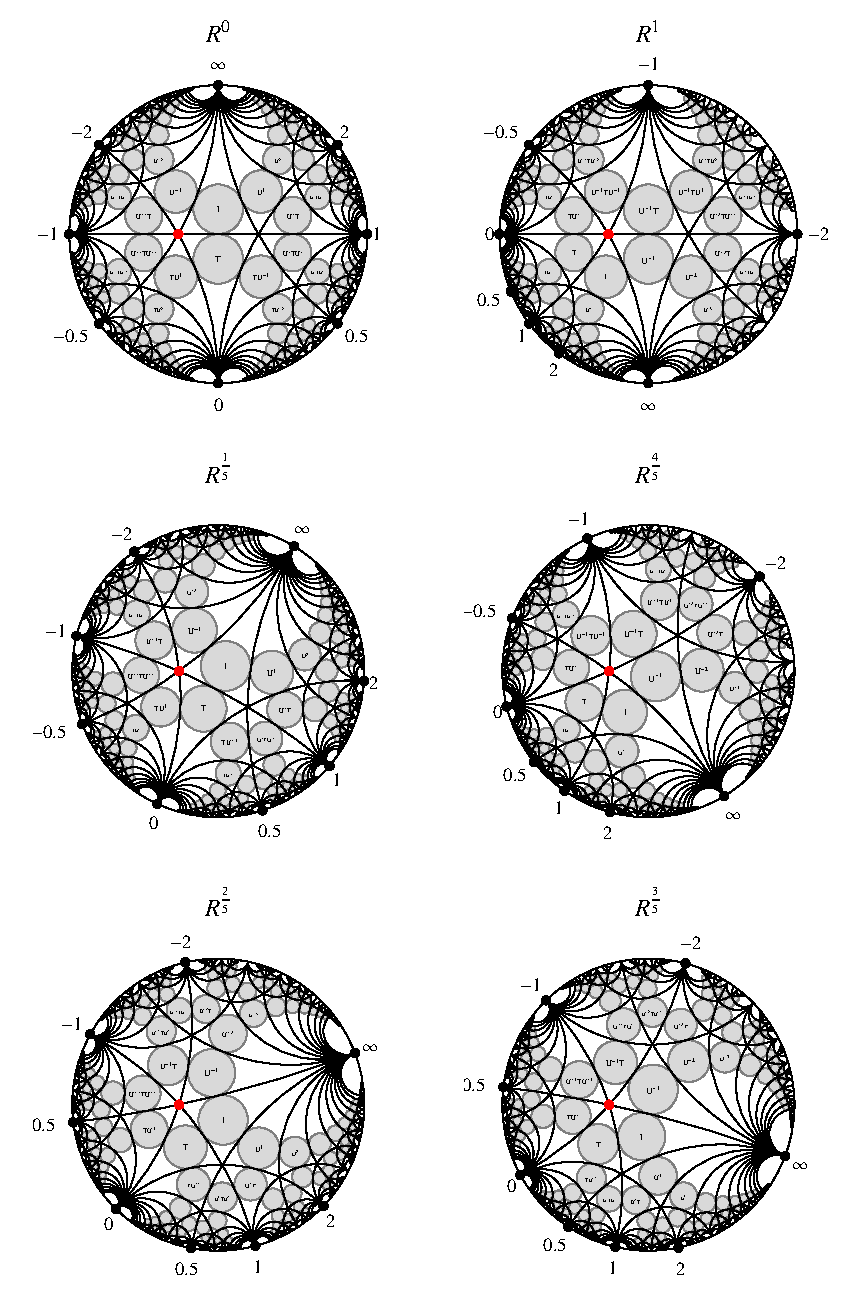
\includegraphics[width=\textwidth]{figures/r-action}
\caption{The action of $R : z \mapsto -\reci{z+1}$.}
\label{fig_RAction}
\end{figure}
\end{example}
\clearpage


% ------------------------------------------------ Section: Continued fractions
\section{The modular group and continued fractions}

For an arbitrary modular transformation $A$, a representation as product of shifts $U^j: z \mapsto z+j$ and inversions $T: z \mapsto -\reci{z}$ can be found by the $T$-$U$ algorithm of Corollary \ref{cor_ModGrpTUAlg}. By writing out this product, for example in the case when $n=2$, we have
\begin{equation*}
A = U^{e_0}T U^{e_1}T U^{e_2}T U^k,
\end{equation*}
or more explicitly
\begin{equation}
\label{eqn_ALongConFrac}
A(z) = e_0 - \reci{e_1 - \reci{e_2 - \reci{k + z}}}.
\end{equation}
\index{Continued fraction}
\index{Pringsheim notation}
Here a close relation between modular transformations and continued fractions immediately gets apparent. In this section we will investigate this relation somewhat deeper. 
First we will use Pringsheim's more space-saving notation for continued fractions, namely
\begin{equation}
\label{eqn_ConFracNotation}
b_0 + \frac{a_1}{b_1 + \frac{a_2}{b_2 + \frac{a_3}{b_3 + \dots}}} =: 
b_0 + \cfr{a_1}{b_1} + \cfr{a_2}{b_2} + \cfr{a_2}{b_3} + \dots
\end{equation}
In the case when all $a_j = 1$, we adhere to the standard sequence notation for continued fractions:
\begin{equation*}
b_0 + \reci{b_1 + \reci{b_2 + \dots}} =: [b_0,b_1,b_2,\dots].
\end{equation*}
\index{Convergent}
For determining a continued fraction representation for a real number $\alpha$ such that all $a_j = 1$, one usually sets $\alpha_0 := \alpha$ as well as $b_j := \floor{\alpha_j}$ and $\alpha_{j+1} := \reci{\alpha_j - b_j}$ for $j \ge 0$ until some $\alpha_j$ is zero (which is the case if and only if $\alpha \in \Q$). In any way we obtain a finite or infinite sequence of equations 
\begin{equation}
\label{eqn_ConFracEqnSeq}
\alpha = \alpha_0 = b_0 + \reci{\alpha_1}, \quad
\alpha_1 = b_1 + \reci{\alpha_2}, \quad
\alpha_2 = b_2 + \reci{\alpha_3}, \quad \dots
\end{equation}
giving rise to the continued fraction representation $\alpha = [b_0, b_1, b_2, \dots]$. The rational number $C_n := [b_0,b_1,\dots,b_n]$ obtained by truncating the continued fraction representation after the coefficient $b_n$, is called the $n$-th \emph{convergent} of the continued fraction. If the continued fraction is infinte, \ie $\alpha \in \R \setminus \Q$, then we have $\lim_{n \to \infty} C_n = \alpha$.

\begin{remark}
\label{rem_ConFracKinds}
\index{Regular continued fraction}
Note that by using the method above, all the coefficients $b_j$ with $j > 0$ are positive. A representation for $\alpha$ of this form is called a \emph{regular continued fraction} -- see also \Lehner{}, �9. 

\index{Semi-regular continued fraction}
In contrast to that, if we set $b_j := \ceil{\alpha_j}$ for some or all of the indices $j$, then also negative coefficients $b_j$, $j > 0$, may occur and we obtain in this way a so called \emph{semi-regular continued fraction} representation of $\alpha$. This is in strong analogy to Remark~\ref{rem_EuclideanAlgorithmRounding} that within the Euclidean algorithm the quotients $q_j$ can be determined by rounding $r_{j-1} / r_j$ either up- or downward. Note that in \Lehner{}, �36, semi-regular continued fractions are defined such that for all $j > 0$ the coefficients $b_j$ are positive, but allowing for $a_j \in \{\pm 1\}$. However this makes no essential difference. 

\index{Canonical continued fraction}
If we use the nearest integer function in each step, \ie $b_j := \nint{\alpha_j}$ for all $j$, then we have $\abs{b_j} \ge 2$ for all $j > 0$. If additionally $\alpha \in \Q$, then it can be shown that the resulting continued fraction representation is one of minimal length -- according to \Lehner{}, �39, we call finite continued fractions with this minimality property \emph{canonical continued fractions}.
\end{remark}

We can now reformulate Corollary \ref{cor_ModGrpTUAlg} in order to construct a continued fraction representation of any given modular transformation.

\begin{corollary}
\label{cor_ModTransConFrac}
An arbitrary modular transformation $A(z) = \moebius{a}{b}{c}{d}{z}$ can be written as continued fraction
\begin{equation}
\label{eqn_ModTransConFrac}
A(z) = [q_0,q_1,\dots,q_n,(-1)^{n+1}(k+z)]
\end{equation}
where the integers $n$, $q_0,q_1,\dots,q_n$ and $k$ are determined by the algorithm described in Corollary \ref{cor_ModGrpTUAlg}.
\end{corollary}
\begin{proof}
By using the continued fraction representation of $A$ given in (\ref{eqn_ALongConFrac}) and by applying the definition $e_j$ := $(-1)^j q_j$, we see
\begin{IEEEeqnarray}{rCcCcCcCcCcCc}
A(z) &=& e_0 &+& \cfr{-1}{e_1} 
          &+& \cfr{-1}{e_2} 
          &+& \dots 
          &+& \cfr{-1}{e_n} 
          &+& \cfr{-1}{k + z} \nonumber \\
  &=& q_0 &+& \cfr{-1}{-q_1} 
          &+& \cfr{-1}{q_2} 
          &+& \dots 
          &+& \cfr{-1}{(-1)^n q_n} 
          &+& \cfr{-1}{k + z}. \label{eqn_ModTransConFracInterim}
\end{IEEEeqnarray}
Now for every odd $j \le n$ we can rewrite 
\begin{equation*}
\cfr{-1}{-q_j} + \cfr{-1}{\dots} \quad \text{to} \quad \cfr{1}{q_j} + \cfr{1}{\dots}.
\end{equation*}
Thus if $n$ is odd, every numerator $-1$ in (\ref{eqn_ModTransConFracInterim}) can be turned into $+1$. In the other case, when $n$ is even, only one negative numerator at the end, $\frac{-1}{k+z}$, remains, but this can easily be rewritten to $\frac{1}{-(k+z)}$. Taking both cases together, we obtain (\ref{eqn_ModTransConFrac}).
\end{proof}

\begin{remark}
\label{rem_TUAlgConFrac}
It is worth noting that determining a continued fraction representation for a rational number $p/q \in \Q$ with $p,q \in \Z$ is essentially equivalent to applying the Euclidean algorithm to the integers $p$ and $q$: If we set $(r_{-1}, r_0) := (p,q)$ and substitute in (\ref{eqn_ConFracEqnSeq}) $\alpha_j = r_{j-1}/r_j$ for all $j \ge 0$, we obtain
\begin{IEEEeqnarray*}{rClCrCl}
\frac{r_{-1}}{r_0} &=& b_0 + \frac{r_1}{r_0} &\quad\Leftrightarrow\quad& 
  r_{-1} &=& b_0 \cdot r_0 + r_1 \\
\frac{r_0}{r_1} &=& b_1 + \frac{r_2}{r_1} &\Leftrightarrow& 
  r_0 &=& b_1 \cdot r_1 + r_2 \\
\frac{r_1}{r_2} &=& b_1 + \frac{r_3}{r_2} &\Leftrightarrow& 
  r_1 &=& b_2 \cdot r_2 + r_3 \\
 &\vdots& & & &\vdots&
\end{IEEEeqnarray*}
In other words, the coefficients $b_j$ of the desired continued fraction representation are nothing else but the quotients of the Euclidean algorithm which we used to denote by $q_j$.

This observation also allows it to see the $T$-$U$ algorithm of Corollary~\ref{cor_ModGrpTUAlg} in a different light: For a given modular transformation $A(z) = \moebius{a}{b}{c}{d}{z}$, by applying the Euclidean algorithm to $a$ and $c$, we effectively determine a continued fraction representation for the rational number $A(\infty) = \frac{a}{c} = [q_0,q_1,\dots,q_n]$. If we set again $e_j := (-1)^j q_j$, it follows that also the modular transformation $P := U^{e_0}T U^{e_1}T\dots U^{e_n}T$ maps $\infty$ to $\frac{a}{c}$. Since the stabilizer of $\infty$ is generated by the transformation $U$, all transformations with this property can be written as $PU^k$ for some $k \in \Z$.
In particular, if we determine the quotients $q_j$ by rounding to the nearest integer, we obtain a \emph{canonical continued fraction}, \ie a continued fraction representation of minimal length -- compare Remark~\ref{rem_ConFracKinds}. Consequently in this case also the product representation returned by the $T$-$U$ algorithm is of minimal length.
\end{remark}

\begin{corollary}
\label{cor_ConFracModTrans}
Given $r \in \EQ$, a transformation $A \in \PSL{\Z}$ satisfying $A(\infty) = r$ can be found by determining a continued fraction representation of $r$, that is $r = [b_0,b_1,\dots,b_n]$, and setting $A := U^{e_0}T U^{e_1}T \dots U^{e_n}T$ where $e_j := (-1)^j b_j$. In particular, the $k$-th convergent $C_k$, $k \le n$, of this continued fraction representation can be written as $C_k = U^{e_0}T U^{e_1}T \dots U^{e_k}T(\infty)$.
\end{corollary}

We have now seen that there is a natural correspondence between rational numbers, continued fractions and the $T$-$U$ word representations of modular transformations. In order to formalize this correspondence, let us denote by $\Words{\Z} := \bigcup_{n \le 0} \Z^n$ the set of finite integer sequences (or words over the alphabet $\Z$). Furthermore we set $\EQ := \Q \cup \{\infty\}$ and define a map $f: \Words{\Z} \to \EQ$ by
\begin{equation}
\label{eqn_ConFracEvalMap}
\fundef{f}{\Words{\Z}}{\EQ}{(b_0,b_1,\dots,b_n)}{[b_0,b_1,\dots,b_n].}
\end{equation}
Note that evaluation of continued fractions shall take place in $\EQ$ with the natural conventions for treating infinite quantities, \ie for $a \ne 0$ and $b \ne \infty$ we have
\begin{equation*}
\frac{a}{0} = \infty,\quad \frac{b}{\infty} = 0,\quad b \pm \infty = \infty.
\end{equation*}
Moreover the empty continued fraction shall evaluate to $\infty$, \ie $f(\epsilon) = \infty$, where $\epsilon \in \Words{\Z}$ denotes the empty sequence. We call the sequence $\beta \in \Words{\Z}$ a \emph{continued fraction representation} for $f(\beta) \in \EQ$. %Two sequences $\beta, \gamma \in \Words{\Z}$ are defined to be \emph{equivalent}, in symbols $\beta \sim \gamma$, if and only if $f(\beta) = f(\gamma)$. 

Next we set $\Syms := \{T,U\} \subseteq \PSL{\Z}$ and let $\FreeGrp{\Syms}$ be the free group generated by the symbols $T$ and $U$. Moreover we denote by $\langle U \rangle$ the subgroup of $\FreeGrp{\Syms}$ which is generated by the symbol $U$ and the subgroup of $\PSL{\Z}$ generated by the transformation $U$. We now consider left cosets of $\langle U \rangle$ in  $\FreeGrp{\Syms}$ and $\PSL{\Z}$:
\begin{eqnarray*}
\FreeGrp{\Syms} / \langle U \rangle &:=& \setdef{\sigma \langle U \rangle}{\sigma \in \FreeGrp{\Syms}},\\
\PSL{\Z} / \langle U \rangle &:=& \setdef{A \langle U \rangle}{A \in \PSL{\Z}}.
\end{eqnarray*}
It is important to note these are \emph{not} factor groups, as $\langle U \rangle$ is not a normal subgroup of $\PSL{\Z}$ or $\FreeGrp{\Syms}$. In particular, neither $\PSL{\Z} / \langle U \rangle$ nor $\FreeGrp{\Syms} / \langle U \rangle$ carry a ``natural'' group structure -- we will regard them just as sets. 

We now have defined all domains needed for writing $f : \Words{\Z} \to \EQ$ as composition of three other functions, namely $f = g_3 \circ g_2 \circ g_1$, where
\begin{IEEEeqnarray*}{rCcCc}
g_1 &:& \Words{\Z} &\to& \FreeGrp{\Syms} / \langle U \rangle, \\
g_2 &:& \FreeGrp{\Syms} / \langle U \rangle &\to& \PSL{\Z} / \langle U \rangle, \\
g_3 &:& \PSL{\Z} / \langle U \rangle &\to& \EQ.
\end{IEEEeqnarray*}
Let us first turn to the definition of $g_1$, which maps a continued fraction representation to a left coset of a certain $T$-$U$ group word.
\begin{equation}
\label{eqn_MapConFracToPath}
\fundef{g_1}{\Words{\Z}}{\FreeGrp{\Syms} / \langle U \rangle}{(b_0,b_2,\dots,b_n)}{U^{e_0}T U^{e_1}T \dots U^{e_n}T \langle U \rangle} \quad \text{where } e_j := (-1)^j b_j.
%\fundef{g_1}{\Words{\Z}}{\FreeGrp{\Syms} / \langle U \rangle}{(b_0,b_2,\dots,b_n)}{\left( \prod_{j=0}^n (U^{e_j}T) \right) \langle U \rangle} \quad \text{where } e_j := (-1)^j b_j.
\end{equation}
Note that in the case of the empty sequence $\epsilon \in \Words{\Z}$ we have $g_1(\epsilon) = \langle U \rangle$.

In order to define $g_2$, let $\phi: \Sigma \to \PSL{\Z}$ be the canonical embedding, \ie $\phi(T) = T$ and $\phi(U) = U$. Let $\overline{\phi}$ be the unique extension of $\phi$ to a homomorphism $\FreeGrp{\Syms} \to \PSL{\Z}$, according to Theorem~\ref{thm_FreeGrpUniqueHom}. Note that $\overline{\phi}$ is just the map which evaluates $T$-$U$ group words to concrete elements of $\PSL{\Z}$ in the obvious way. The function $g_2$ now takes  a left coset in $\FreeGrp{\Syms}$ to a left coset in $\PSL{\Z}$ by
\begin{equation}
\label{eqn_MapPathToCoset}
\fundef{g_2}{\FreeGrp{\Syms} / \langle U \rangle}{\PSL{\Z} / \langle U \rangle}{\sigma \langle U \rangle}{\overline{\phi}(\sigma) \langle U \rangle.}
\end{equation}
Last but not least we define $g_3$ as the map which evaluates the transformations of a left coset $A \langle U \rangle \in \PSL{\Z} / \langle U \rangle$ at the point $\infty$. Note that the result is the same for all transformations within one coset because $\langle U \rangle$ is exactly the stabilizer of $\infty$, \ie $\langle U \rangle = \setdef{B \in \PSL{\Z}}{B(\infty) = \infty}$. This allows us to define
\begin{equation}
\label{eqn_MapCosetToEQ}
\fundef{g_3}{\PSL{\Z} / \langle U \rangle}{\EQ}{A \langle U \rangle}{A(\infty).}
\end{equation}

\begin{lemma}
\label{lem_ConFracMapEquality}
The maps $g_1$, $g_2$, $g_3$ and $f$, defined as above, satisfy
\begin{equation*}
f = g_3 \circ g_2 \circ g_1.
\end{equation*}
\end{lemma}
\begin{proof}
It follows from Corollary~\ref{cor_ModTransConFrac} and Remark~\ref{rem_TUAlgConFrac} that the composed map $g_2 \circ g_1: \Words{\Z} \to \PSL{\Z} / \langle U \rangle$ takes a continued fraction representation $(b_0,b_1,\dots,b_n)$ to the set of all modular transformations of the form $A(z) = [b_0,b_1,\dots,b_n,(-1)^{n+1}(k + z)]$, $k \in \Z$. Evaluating these transformations at the point $\infty$ obviously yields the rational number $[b_0,b_1,\dots,b_n]$ and we have indeed $f = g_3 \circ g_2 \circ g_1$.
\end{proof}

\begin{lemma}
\label{lem_MapConFracToPathInjective}
The map $g_1$ defined in (\ref{eqn_MapConFracToPath}) is injective. Its image $g_1(\Words{\Z})$ consists precisely of those cosets $\sigma \langle U \rangle \in \FreeGrp{\Syms} / \langle U \rangle$, where the $T$-$U$ group word $\sigma$ is such that:
\begin{enumerate}[\quad(i)]
\item \label{itm_NotContainsTInv}
The reduced form of $\sigma$ never contains the symbol $\inv{T}$.
\item \label{itm_RightmostIsT}
If the reduced form of $\sigma$ is not empty, its rightmost symbol is $T$.
\end{enumerate}
In particular there is a one-to-one correspondence between all continued fraction representations and $T$-$U$ group words of this form. 
\end{lemma}
\begin{proof}
The fact that $g_1$ is injective is obvious. It is also clear that the word
\begin{equation}
\label{eqn_MapConFracToPathImageWord}
U^{e_0}T U^{e_1}T \dots U^{e_n} T
\end{equation}
with $n \ge 0$, $e_j \in \Z$ occurring in the definition of $g_1$ is already reduced and satisfies (\ref{itm_NotContainsTInv}) and (\ref{itm_RightmostIsT}). Conversely, every reduced word $w$ satisfying (\ref{itm_NotContainsTInv}) and (\ref{itm_RightmostIsT}) has necessarily the form
\begin{equation*}
w = U^{k_1} T^{\ell_1} U^{k_2} T^{\ell_2} \dots U^{k_m} T^{\ell_m},
\end{equation*}
with $m >= 0$, $k_j \in \Z$ and $\ell_j \ge 1$. Because for $k \ge 1$, $T^k$ and $(TU^0)^{k-1}T$ are \emph{identical} as words, we can for sure notate $w$ alternatively in the form (\ref{eqn_MapConFracToPathImageWord}).
\end{proof}

\begin{lemma}
\label{lem_MapCosetToEQBijective}
The map $g_3$ defined in (\ref{eqn_MapCosetToEQ}) is bijective. In particular there is a one-to-one correspondence between the left cosets of $\langle U \rangle$ in $\PSL{\Z}$ and the extended rational numbers $\EQ$.
\end{lemma}
\begin{proof}
If $g_3(A \langle U \rangle) = g_3(B \langle U \rangle)$, then $A(\infty) = B (\infty)$. This is equivalent to $\inv{B}A \in \langle U \rangle$ or $A \langle U \rangle = B \langle U \rangle$. Therefore $g_3$ is injective. Since $f = g_3 \circ g_2 \circ g_1$ is surjective, the same must be true for $g_3$.
\end{proof}

\begin{figure}
\centering
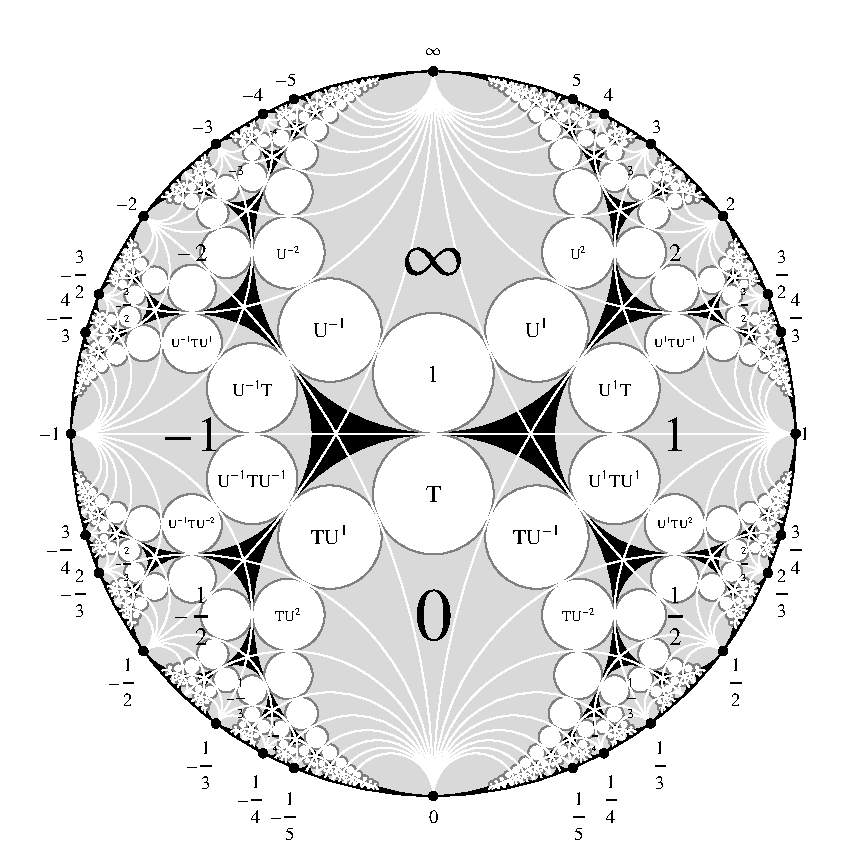
\includegraphics[width=\textwidth]{figures/ford-disks}
\caption{Todo.}
\label{fig_FordDisks}
\end{figure}
Looking at the modular tessellation, Figure~\ref{fig_ModularTiling}, we see that the images of the indisk $\Indisk$ of the fundamental region $\FunDom$ 
have a natural one-to-one correspondence to modular transformations, \ie the disk $A\Indisk$ can be considered as a graphical representative for the modular transformation $A$. 

The question arises, if there is such a visual and clear representation also for left cosets of $\langle U \rangle$ in $\PSL{\Z}$. Indeed, we can see in Figure~\ref{fig_FordDisks}, depicting the modular tessellation under the modified Cayley transform, that the disks $U^k\Indisk$, $k \in \Z$ form a ``generalized ring'' which asymptotically approaches the point $\infty$. We can enclose this ring in a generalized disk -- in Figure~\ref{fig_FordDisks}, this enclosing disk is shown in light gray and is labeled with ``$\infty$''.
\begin{definition}
\label{dfn_FordDisk}
\index{Ford disk}
The unique (open) g-disk $\Forddisk_\infty$ containing all the disks $U^k\Indisk$, $k \in \Z$, in its interior and being tangent to each of them is called the \emph{Ford disk at $\infty$}. It contains all points $z \in \C$ with $\Im{z} > 1$. Its defining matrix is given by
\begin{equation}
\label{eqn_FordDisk}
\Forddisk_\infty = \mat{0}{-\ii}{\ii}{2}.
\end{equation}
For a modular transformation $A = \smallmat{a}{b}{c}{d} \in \PSL{\Z}$, the image of $\Forddisk_\infty$ under $A$ is called the \emph{Ford disk at $\frac{a}{c}$}, $\Forddisk_{\frac{a}{c}} := A\Forddisk_\infty$.
\end{definition}

The above definition as well as the bijective correspondence between left cosets of $\langle U \rangle$ in $\PSL{\Z}$ and the extended rational numbers $\EQ$ (Lemma~\ref{lem_MapCosetToEQBijective}) will get much clearer in view of Figure~\ref{fig_FordDisks}: We can see that every Ford disk $\Forddisk_r$ (the disk in light gray labeled with $r$), ``touches'' the extended real axis $\R_\infty := \R \cup \{\infty\}$ (appearing as unit circle under the modified Cayley transform) exactly in the point $r$, that is
\begin{equation*}
\topcl{\Forddisk_r} \cap \R_\infty = \{r\} \quad \text{for all } r \in \EQ.
\end{equation*}
For the seeing the relation of Ford disks to left costets of $\langle U \rangle$ in $\PSL{\Z}$, first observe that the Ford disk $\Forddisk_\infty$ contains all the indisks $U^k \Indisk$, $k \in \Z$. We may notate this fact concisely as $\langle U \rangle \Indisk \subseteq \Forddisk_\infty$. In this sense, we can consider $\Forddisk_\infty$ as a graphical representative for the subgroup $\langle U \rangle$ of $\PSL{\Z}$. Clearly every Ford disk $\Forddisk_r$ is the image of $\Forddisk_\infty$ under some transformation $A \in \PSL{\Z}$ (which can be found using Corollary~\ref{cor_ConFracModTrans}), \ie $A\Forddisk_\infty = \Forddisk_r$. Consequently $A \langle U \rangle \Indisk \subseteq \Forddisk_r$ and we can therefore consider $\Forddisk_r$ as graphical representative for the coset $A \langle U \rangle$.

Also Lemma~\ref{lem_MapConFracToPathInjective}, establishing a one-to-one correspondence between continued fraction representations and certain $T$-$U$ words, has a nice visual interpretation, as we will illustrate in the following example.

\begin{figure}
\centering
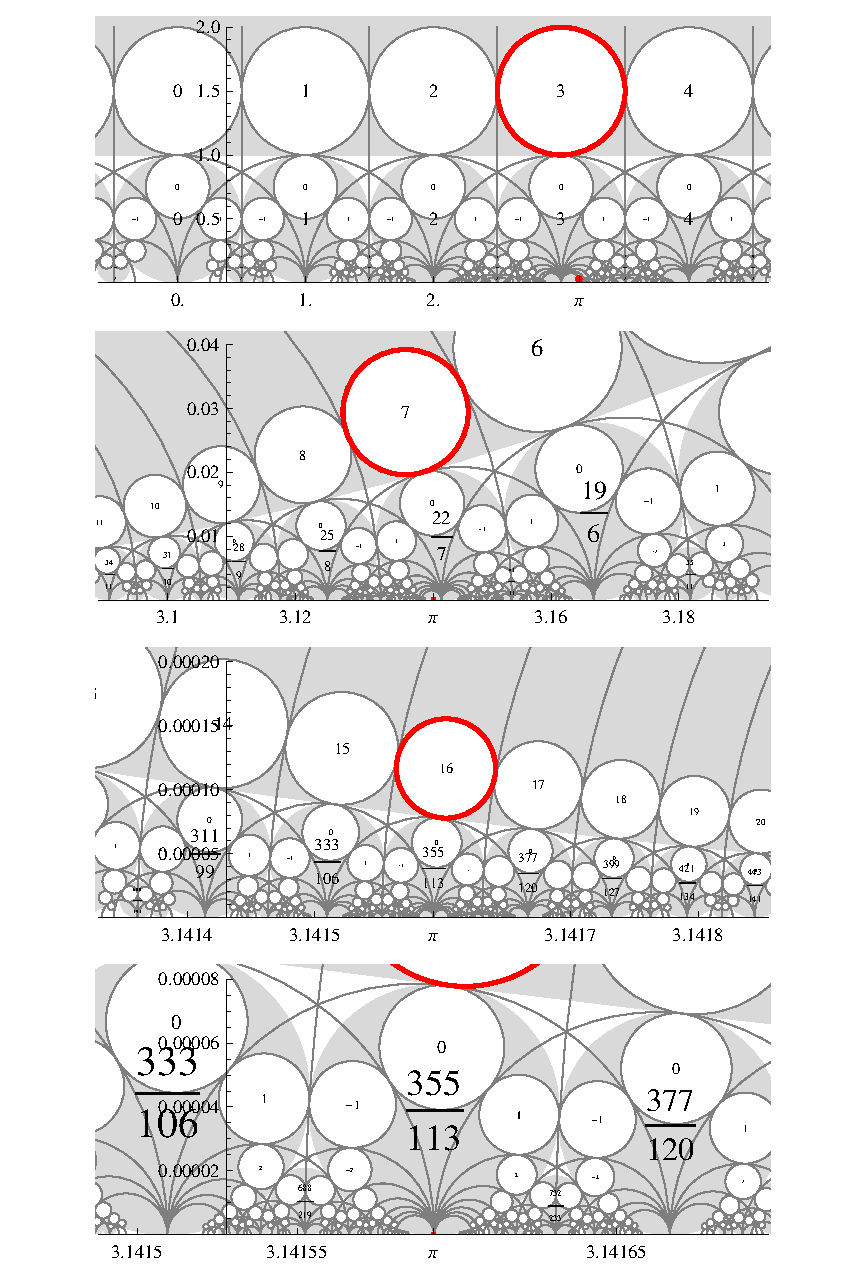
\includegraphics[width=\textwidth]{figures/cont-frac-pi}
\caption{$\pi = \frac{355}{113}$ -- well, almost.}
\label{fig_ConFracPi}
\end{figure}
\begin{example}
\label{ex_ConFracPi}
Consider the (semi-regular) continued fraction expansion of the irrational number $\pi$, obtained by using the nearest integer function for rounding the $\alpha_j$ -- compare Remark~\ref{rem_ConFracKinds}. The first few coefficients of this continued fraction are given by
\begin{equation*}
\pi = [3, 7, 16, -294, 3, -4, 5, -15, -3, 2, 2, 2, 2, 3, -85, -3, 2, 15, 3, 14,\dots]
\end{equation*}
More coefficients can be found when looking up the sequence A133593 on the \emph{On-Line Encyclopedia of Integer Sequences (OEIS)}\footnote{https://oeis.org}. The convergents of this continued fraction give (by Corollary~\ref{cor_ConFracModTrans}) rise to a sequence of Modular transformations:
\begin{IEEEeqnarray*}{rCcCl}
\lbrack 3 \rbrack &=& 3
  &=& U^3 T (\infty),\\
\lbrack 3,7 \rbrack &=& \frac{22}{7} 
  &=& U^3 T U^{-7} T (\infty),\\
\lbrack 3,7,16 \rbrack &=& \frac{355}{113}
  &=& U^3 T U^{-7} T U^{16} T (\infty),\\
\lbrack 3,7,16,-294 \rbrack &=& \frac{104348}{33215} 
  &=& U^3 T U^{-7} T U^{16} T U^{294} T (\infty),\\
&\vdots& &\vdots&
\end{IEEEeqnarray*}
\end{example}


\todo{19}{The modular group and ford circles}


% ------------------------- Section: Modular tiling, exponential transformation
\section{The modular tessellation and the exponential transformation}

In the theory of modular functions, which we will touch in the next section,
a map of essential importance is the transformation $z \mapsto \exp(2 \pi \ii z)$. Adopting the notation of \Lehner{}, we will denote this transformation by
\begin{equation}
\ex(z) := \exp\left(2 \pi \ii z \right).
%\fundef{\ex}{\C}{\C}{z}{\exp\left(2 \pi \ii z\right)}.
\end{equation}
Just like the Cayley transform, $\ex$ maps the upper half-plane onto the unit disk $\mathbb{D}$, as we see through
\begin{equation*}
\abs{\ex(z)} = 
\exp\left(\Re{2 \pi \ii z}\right) = 
\exp\left(-2 \pi \Im{z}\right).
\end{equation*}
Obviously $\Im{z} > 0$ implies $\abs{\ex(z)} < 1$. The real axis is mapped to the boundary of $\mathbb{D}$. In contrast to the Cayley transform, $e$ is not a one-to-one map from the upper half-plane to the unit disk, as clearly $e(z) = e(z + k)$ for arbitrary $k \in \Z$. Instead it can be considered as a bijective map from the strip 
\begin{equation*}
S = \setdefsz{\big}{z \in \C}{\Re{z} \in \left[-0.5,0.5\right),\ \Im{z} \ge 0}
\end{equation*}
to the punctured unit disk $\mathbb{D} \setminus \{0\}$. Note that the exponential function has an essential singularity at the point $\infty$, but still it is sometimes useful to define $e(\infty) := 0$. This is motivated by a continuous extension of $e$ from the domain $S$ to $S_\infty := S \cup \{\infty\}$ by
\begin{equation*}
e(\infty) := \lim_{\substack{\Im{z} \to \infty\\z \in S}} e(z) = 0.
\end{equation*}
In this way we obtain a bijective map from the set $S_\infty$ to the closed unit disk $\mathbb{D}$ which can be used to map the modular tessellation of the upper half-plane -- to be precise, the part of it which lies within $S_\infty$ -- to the unit disk as shown in Figure~\ref{fig_ModularTilingExp}. 
\begin{figure}
\centering
\includegraphics[width=\textwidth]{figures/modular-tiling-exp}
\caption[The modular tessellation under the map $z \mapsto \ex(z)$]{The modular tessellation under the transformation $z \mapsto e(z)$. The equation $\abs{z} = \exp(-2\pi \ii \Im{z})$ implies that points with large imaginary part are mapped very closely to $0$. For this reason, the image of the fundamental domain $\FunDom$ cannot be seen any more in this scale. Its points, satisfying $\Im{z} > \frac{\sqrt{3}}{2}$, are mapped into a disk centered about the origin of a radius smaller than $0.005$.}
\label{fig_ModularTilingExp}
\end{figure}

\begin{remark}
In order to trace the image of the fundamental domain $\FunDom$ and its indisk $\Indisk$ under the map $\ex$, we have to zoom in on the neighborhood of zero, which is done in Figure~\ref{fig_ModularTilingExpZoom}. The top-left frame again shows the image of the tessellation under $\ex$ on the whole unit disk. 

The second frame displays the images of the regions $TU\FunDom$ and $T\inv{U}\FunDom$ in more detail. Comparing with Figure~\ref{fig_ModularTiling}, we see that originally these two regions do not have any boundary arc in common. However, due to the periodicity of $e$, the left boundary arc of $TU\FunDom$ (being a segment of the line $\Re{z} = -1/2$) and the right boundary arc of $T\inv{U}\FunDom$ (being a segment of the line $\Re{z} = 1/2$) have the same image under the transformation $\ex$. Therefore the images of $TU\FunDom$ and $T\inv{U}\FunDom$ touch each other along a certain interval on the negative real axis. 

The third frame reveals some more detail on the real shape of $e(T\FunDom)$. Its ``tip'' is not round, as a short look on the first two frames might suggest, but in fact it has a kink at the point $\ex(\rho) = \ex(T\rho) \approx -0.0043$. Moreover, the image of $T\FunDom$ completely surrounds the image of the fundamental domain $\FunDom$ as we see in the next frame: 

Denoting the boundary arcs of $\FunDom$ by $a,b,c$ and $d$ as in Figure~\ref{fig_FunDomGenDisks}, we can see in the fourth frame the image of the left boundary arc $a$ and the right boundary arc $b$ of $\FunDom$ are both mapped to the same interval $[\ex(\rho), 0]$ on the negative real axis. The images of the unit circle arcs $c$ and $d$ form the drop-shaped boundary of $\ex(\FunDom)$. Note that $\ex(c)$ constitutes the part of the boundary in the lower half-plane and $\ex(d)$ the part in the upper half-plane. 

Finally in the last row, we can see the image of the indisk $\Indisk$ in detail. Note that the transformed indisk touches itself in the point $\ex(\pm\half{1} + \half{3}\ii) \approx -0.00008$. The points within $\FunDom$ lying ``above'' $\Indisk$ (including the point $\infty$) are mapped to just another tiny drop-shaped region surrounded entirely by $\ex(\Indisk)$.

\begin{figure}
\centering
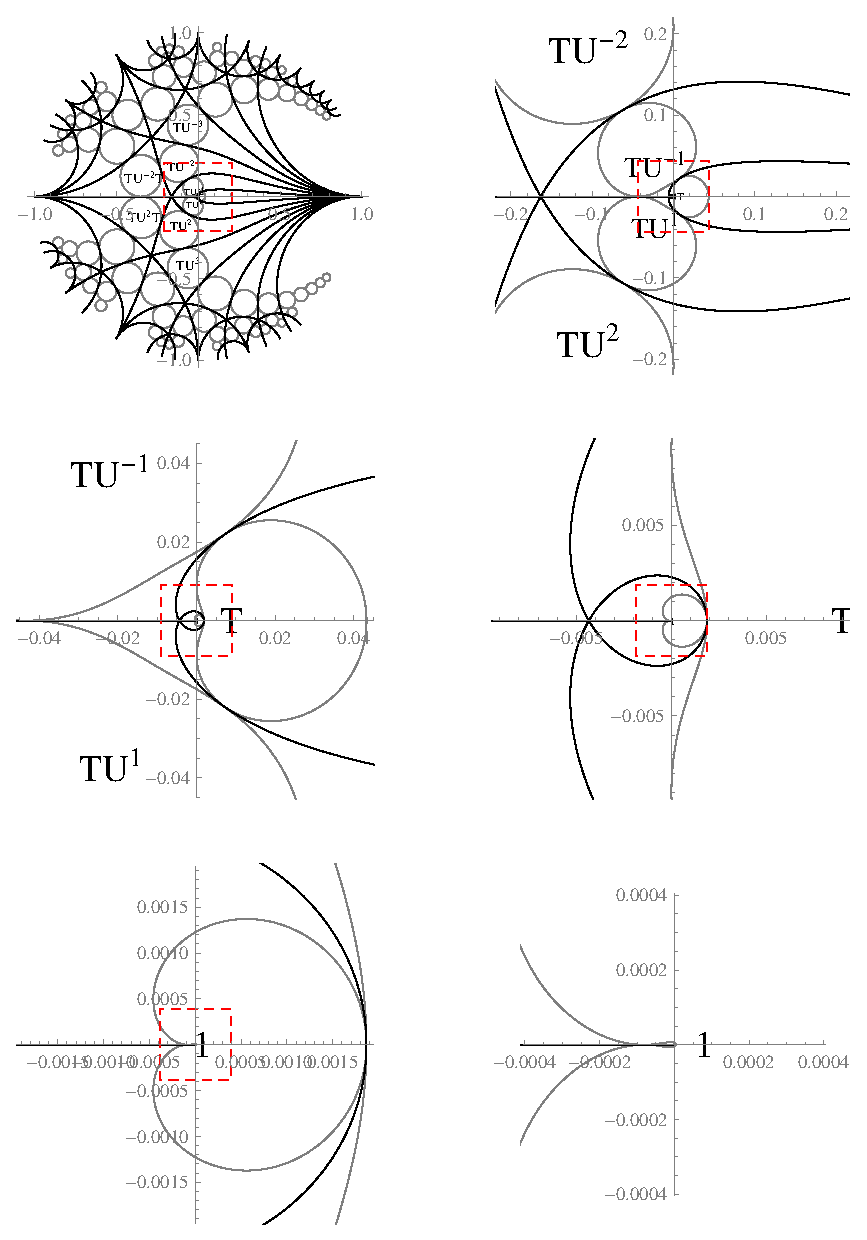
\includegraphics[width=0.95\textwidth]{figures/modular-tiling-exp-zoom}
\caption[The fundamental domain $\FunDom$ and its indisk $\Indisk$ under the map $z \mapsto \ex(z)$]{The image of the fundamental domain $\FunDom$ and its indisk $\Indisk$ under the map $z \mapsto \ex(z)$ can be seen by zooming in to a close neighborhood of $0$.}
\label{fig_ModularTilingExpZoom}
\end{figure}
\end{remark}

Having studied the image of the modular tessellation under the transformation $z \mapsto \ex(z)$ in detail, the question arises whether this relates somehow to the image of the tessellation under the modified Cayley transform $\ModCayley$ which we have seen in Figure~\ref{fig_ModularTiling}. Indeed it is possible to visualize the connection between these two images. For this purpose we take advantage of yet another M�bius transformation:
\begin{equation}
f(z) := \frac{\ii}{z + \\i} = -\half{\ii} \ModCayley(z) + \half{1}.
\end{equation}
As we see, $f$ can be considered as composition of the modified Cayley transform, a clockwise rotation by $90^\circ$, scaling by the factor $\reci{2}$ and a final translation by $\reci{2}$. Therefore, $f$ maps the upper half-plane to a disk of radius $\reci{2}$ centered about the real point $\reci{2}$. The choice of $f$ is not as arbitrary as it first might seem, because
\begin{equation*}
f(0) = \ex(0) = 1 \quad\text{and}\quad f(\infty) = \ex(\infty) = 0.
\end{equation*}
This property allows it to establish a continuous transition between the images of the tessellation under $f$ and $\ex$ which leaves the points $0$ and $1$ fixed. For this purpose we may for example use the map
\begin{equation}
h(t, z) := f(z)^{1-t} \cdot \ex(tz),
\end{equation}
with varying parameter $t \in [0,1]$. Note that complex powers $z^t$, $z \in \C$, $t \in \R$ shall be evaluated as $\exp(t \ln z)$, by choosing a branch of the natural logarithm such that the imaginary part of the logarithm ranges in the interval $(-\pi, \pi]$. Moreover, for $z = \infty$ we define $h(t, \infty) := f(\infty) = \ex(\infty) = 0$.

In Figure~\ref{fig_ModularTilingExpFan}, we can see the images the modular tessellation under the map $h(t,\cdot)$ for the parameter values $t \in \{0,\reci{5},\frac{2}{5},\frac{3}{5},\frac{4}{5},1\}$. In the first frame, we see that the image of the tessellation under $h(0,\cdot) = f$ is indeed a rotated and scaled version of the one belonging to $\ModCayley$, when omitting the part which lies outside the strip $\abs{\Re{z}} \le \reci{2}$ (compare Figure~\ref{fig_ModularTiling}). 

As the parameter value $t$ is stepwise increased in the following frames, the image is slowly fanned out to the whole unit disk. Finally we end up with the image of the tessellation under $h(1,\cdot) = \ex$.
\begin{figure}
\centering
\includegraphics[width=0.9\textwidth]{figures/modular-tiling-exp-fan}
\caption[The modular Pac-Man]{The modular tessellation on the strip $\abs{\Re{z}} \le \reci{2}$ under the maps $z \mapsto f(z) = \frac{\ii}{z + \\i}$ (top-left) and under $z \mapsto \ex(z)$ (bottom-right). A continuous transition between these two images is established through the map $h(t,z) = f(z)^{1-t} \cdot \ex(tz)$ when the parameter $t \in [0,1]$ is varied.}
\label{fig_ModularTilingExpFan}
\end{figure}

\begin{remark}
In a more general context, the connection between a region $R$ of similar shape as above (\ie a region bounded by three circular arcs having vertex angles $90^\circ$, $90^\circ$ and $0^\circ$), a M�bius transformation leaving the vertex with angle $0^\circ$ fixed and an exponential transformation which maps $R$ to the unit disk, is discussed in \Lehner{}, p.\ 68ff.
\end{remark}
\clearpage


% -------------------------------------------------- Section: Klein j invariant
\section{Modular functions}

We devote the last section of this thesis to the visualization of modular functions. Without diving deeply into their theory -- which is treated  comprehensively in \Schoeneberg{} -- just enjoying the visual aesthetics of the arising figures might give an idea on the mathematical importance and beauty of modular functions.

\index{Meromorphic function}
Modular functions are meromorphic maps (\ie maps which are holomorphic\footnote{Instead of ``holomorphic'' the term ``analytic'' is also frequently used.} except for isolated poles, or in other words, maps which can be represented as quotient of two holomorphic functions) defined on the upper half-plane and satisfying a symmetry relation which is induced by the transformations of the modular group.

\begin{definition}[Modular function]
Let the upper halfplane $\mathcal{H}$ and the extended upper halfplane $\EU$ be defined as in (\ref{eqn_Upperhalfplane}) and (\ref{eqn_ExtUpperhalfplane}) respectively.
A map $f : \EU \to \EC$ is called a \emph{modular function}, if it satisfies the following conditions:
\begin{enumerate}[\quad(i)]
\item $f$ is meromorphic on the upper half-plane $\mathcal{H}$.
\item $f$ satisfies $f = f \circ A$ for all $A \in \PSL{\Z}$.
\item There exists a $k_0 \in \Z$, a sequence $(a_k)_{k \ge k_0}$, $a_k \in \C$ with $a_{k_0} \ne 0$ and a constant $C > 0$ such that $f$ has a series expansion of the form
\begin{equation*}
f(z) = \sum_{k \ge k_0} a_k \ex(k z) \quad \text{for all } z \in \C \text{ with } \Im{z} > C,
\end{equation*}
where the transformation $\ex : \C \to \C$ is defined as in (\ref{eqn_ExponentialTransform}).
\end{enumerate}
\end{definition}

\begin{figure}
\centering
\includegraphics[width=0.8\textwidth]{figures/klein-j}
\caption{The composition of the Klein modular invariant function and the inverse modified Cayley transform $j \circ \inv{\ModCayley}$.}
\label{fig_KleinJ}
\end{figure}

\begin{figure}
\centering
\begin{tabular}{c c c}
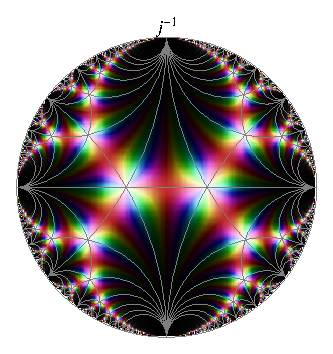
\includegraphics[width=0.45\textwidth]{figures/klein-jinv} & \quad &
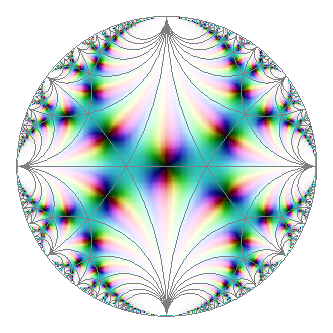
\includegraphics[width=0.45\textwidth]{figures/klein-jm1} \\
\\
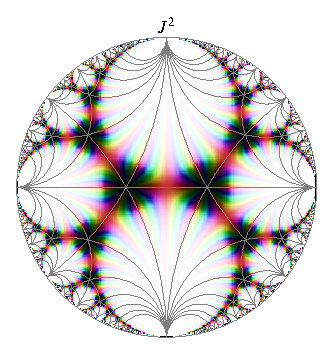
\includegraphics[width=0.45\textwidth]{figures/klein-jsqr} & \quad &
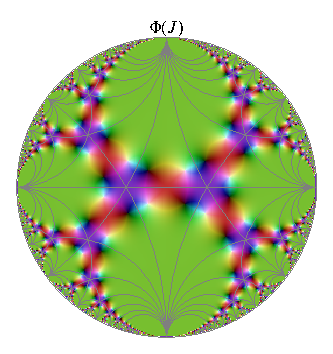
\includegraphics[width=0.45\textwidth]{figures/klein-j-mod-cayley}
\end{tabular}
\caption{The composition of the Klein modular invariant function and the inverse modified Cayley transform $j \circ \inv{\ModCayley}$.}
\label{fig_FunctionsOfJ}
\end{figure}

\begin{figure}
\centering
\includegraphics[width=0.8\textwidth]{figures/klein-jfib-large}
\caption{The composition of the Klein modular invariant function and the inverse modified Cayley transform $j \circ \inv{\ModCayley}$.}
\label{fig_KleinJFib}
\end{figure}


\backmatter

\printindex

\bibliographystyle{plain}
\bibliography{literature}

\begin{appendices}
\chapter{Errors and modifications}

In comparison to the officially submitted diploma thesis, the following changes have been made in this revised version:

\begin{description}
\correction{\pageref{err_TRsign}}{Forgotten minus sign}
{\dots in terms of the transformations $T : z \mapsto \reci{z}$, $U : z \mapsto z+1$ and $R : z \mapsto \reci{z+1}$.}
{\dots in terms of the transformations $T : z \mapsto -\reci{z}$, $U : z \mapsto z+1$ and $R : z \mapsto -\reci{z+1}$.}

\correction{\pageref{err_TildeFunDom}}{Wrong definition}
{For the proof that the region $\FunDom := \setdef{z \in \C}{\abs{\Re{z}} < 1 \land \abs{z} > 1}$ is a fundamental region \dots}
{For the proof that the region $\FunDom$ defined on page \pageref{eqn_PSL2FunDom} is a fundamental region \dots}

\correction{\pageref{err_SuperfluousOne}}{Superfluous word; $bc$ instead of $bd$}
{Therefore, if one the predicate $t(A)$ is satisfied, then at least one of the two inequalities involved is \emph{strictly} fulfilled, \ie $ac > 0$ or $bc > 0$.}
{Therefore, if the predicate $t(A)$ is satisfied, then at least one of the two inequalities involved is \emph{strictly} fulfilled, \ie $ac > 0$ or $bd > 0$.}

\correction{\pageref{err_dfn_FunDom}}{imprecise definition}
{\dots if the neighborhood of every boundary point \dots}
{\dots if every neighborhood of every boundary point \dots}

\correction{\pageref{err_adbcInsteadOfabcd}}{$ad$ and $bc$ instead of $ab$ and $cd$}
{\dots, \ie also the terms $ad$ and  $bc$ have non-opposite signs, \dots}
{\dots, \ie also the terms $ab$ and $cd$ have non-opposite signs, \dots}

\correction{\pageref{itm_SL2FunDomObsB}}{$bc$ instead of $cd$}
{(\ref{itm_SL2FunDomObsB})\quad
$\abs{ab} = 0$ implies $\abs{bc} \ne 0$ (and vice versa).}
{(\ref{itm_SL2FunDomObsB})\quad
$\abs{ab} = 0$ implies $\abs{cd} \ne 0$ (and vice versa).}

\correction{\pageref{err_x0Missing}}{$x_0$ missing}
{$y := x_n = TU^{-e_n} TU^{-e_{n-1}} \cdots TU^{-e_0} = \dots$}
{$y := x_n = TU^{-e_n} TU^{-e_{n-1}} \cdots TU^{-e_0} x_0 = \dots$}

\modification{\pageref{mod_yDefClarity}}{Minor modification for clarity}
{$TU^{-e_n} \cdots TU^{-e_1} TU^{-e_0} x_0 = x_n.$ \quad Since the vector $y := x_n$ satisfies \dots}
{$y := x_n = TU^{-e_n} \cdots TU^{-e_1} TU^{-e_0} x_0.$ \quad Since the vector $y$ satisfies \dots}

\modification{\pageref{fig_PSL2MinRegion}}{Simplification}
{Figure \ref{fig_PSL2MinRegion}: The region $\mathcal{R} \subseteq \EC$ of numbers $z = u/v \in \EC$ with $\abs{u\conj{v} + \conj{u}v} < \min\{\abs{u}^2,\abs{v}^2\}$.}
{Figure \ref{fig_PSL2MinRegion}: The region $\mathcal{R}$ of numbers $z \in \C$ with $\abs{z + \conj{z}} < \min\{\abs{z}^2, 1\}$.}

\modification{\pageref{eqn_PSL2MinRegion}}{Clarification}
{$\mathcal{R} := \pi\left(\hat{\mathcal{R}}\right) = 
\setdefsz{\Big}{\frac{u}{v} \in \EC}{\abs{u\conj{v} + \conj{u}v} < \min\{\abs{u}^2, \abs{v}^2\}}.$}
{$\mathcal{R} := \pi\left(\hat{\mathcal{R}}\right) = 
\setdefsz{\Big}{z \in \C}{\abs{z + \conj{z}} < \min\{\abs{z}^2, 1\}}.$}

\correction{\pageref{err_leInsteadOflt}}{``$\le$'' instead of ``$<$''}
{\dots{} shall be characterized by the property $\hypdist{z}{z_0} \le \hypdist{Az}{z_0}$ \dots}
{\dots{} shall be characterized by the property $\hypdist{z}{z_0} < \hypdist{Az}{z_0}$ \dots}

\item[Page \pageref{err_PiApprox}]: $\frac{355}{133}$ is \emph{not} a good approximation for $\pi$. Corrected (2 times): $\frac{355}{113}$.

\correction{\pageref{err_fLowerCase}}{$f$ instead of $F$}
{(iii) \dots{} Moreover, \quad $f(\infty) = \dots$}
{(iii) \dots{} Moreover, \quad $F(\infty) = \dots$}

\end{description}

\end{appendices}

\end{document}
